% Siconos-Doc version 3.0.0, Copyright INRIA 2005-2008.
% Siconos is a program dedicated to modeling, simulation and control
% of non smooth dynamical systems.	
% Siconos is a free software; you can redistribute it and/or modify
% it under the terms of the GNU General Public License as published by
% the Free Software Foundation; either version 2 of the License, or
% (at your option) any later version.
% Siconos is distributed in the hope that it will be useful,
% but WITHOUT ANY WARRANTY; without even the implied warranty of
% MERCHANTABILITY or FITNESS FOR A PARTICULAR PURPOSE.  See the
% GNU General Public License for more details.
%
% You should have received a copy of the GNU General Public License
% along with Siconos; if not, write to the Free Software
% Foundation, Inc., 51 Franklin St, Fifth Floor, Boston, MA  02110-1301  USA
%
% Contact: Vincent ACARY vincent.acary@inrialpes.fr 
%/
\documentclass[10pt]{report}
%$Id: macro.tex,v 1.10 2004/12/08 13:38:58 acary Exp $


%\usepackage{a4wide}
\textheight 25cm
\textwidth 16.5cm
\topmargin -1cm
%\evensidemargin 0cm
\oddsidemargin 0cm
\evensidemargin0cm
\usepackage{layout}


\usepackage{amsmath}
\usepackage{amssymb}
\usepackage{minitoc}
%\usepackage{glosstex}
\usepackage{colortbl}
\usepackage{hhline}
\usepackage{longtable}

%\usepackage{glosstex}
%\def\glossaryname{Glossary of Notation}
\def\listacronymname{Acronyms}

\usepackage[outerbars]{changebar}\setcounter{changebargrey}{20}
%\glxitemorderdefault{acr}{l}

%\usepackage{color}
\usepackage{graphicx,epsfig}
\graphicspath{{./Figures/}}
\usepackage[T1]{fontenc}
\usepackage{rotating}

%\usepackage{algorithmic}
%\usepackage{algorithm}
\usepackage{ntheorem}
\usepackage{natbib}


%\renewcommand{\baselinestretch}{2.0}
\setcounter{tocdepth}{2}     % Dans la table des matieres
\setcounter{secnumdepth}{3}  % Avec un numero.



\newtheorem{definition}{Definition}
\newtheorem{lemma}{Lemma}
\newtheorem{claim}{Claim}
\newtheorem{remark}{Remark}
\newtheorem{assumption}{Assumption}
\newtheorem{example}{Example}
\newtheorem{conjecture}{Conjecture}
\newtheorem{corollary}{Corollary}
\newtheorem{OP}{OP}
\newtheorem{problem}{Problem}
\newtheorem{theorem}{Theorem}


\newcommand{\CC}{\mbox{\rm $~\vrule height6.6pt width0.5pt depth0.25pt\!\!$C}}
\newcommand{\ZZ}{\mbox{\rm \lower0.3pt\hbox{$\angle\!\!\!$}Z}}
\newcommand{\RR}{\mbox{\rm $I\!\!R$}}
\newcommand{\NN}{\mbox{\rm $I\!\!N$}}

\newcommand{\Mnn}{\mathcal M^{n\times n}}
\newcommand{\Mnp}[2]{\ensuremath{\mathcal M^{#1\times #2}}}



\newcommand{\Frac}[2]{\displaystyle \frac{#1}{#2}}

\newcommand{\DP}[2]{\displaystyle \frac{\partial {#1}}{\partial {#2}}}

% c++ variables writting
\newcommand{\varcpp}[1]{\textit{#1}}
% itemize
\newcommand{\bei}{\begin{itemize}}
\newcommand{\ei}{\end{itemize}}

\newcommand{\ie}{i.e.}
\newcommand{\eg}{e.g.}
\newcommand{\cf}{c.f.}
\newcommand{\putidx}[1]{\index{#1}\textit{#1}}

\def\Er{{\rm I\! R}}
\def\En{{\rm I\! N}} 
\def\Ec{{\rm I\! C}}
 
\def\zc{\hat{z}}
\def\wc{\hat{w}}

\font\tete=cmr8 at 8 pt
\font\titre= cmr12 at 20 pt 
\font\titregras=cmbx12 at 20 pt

%----------------------------------------------------------------------
%                  Modification des subsubsections
%----------------------------------------------------------------------
\makeatletter
\renewcommand\thesubsubsection{\thesubsection.\@alph\c@subsubsection}
\makeatother

%----------------------------------------------------------------------
%             Redaction note environnement
%----------------------------------------------------------------------
\makeatletter
\theoremheaderfont{\scshape}
\theoremstyle{marginbreak}
\theorembodyfont{\upshape}
%\newtheorem{rque}{\bf Remarque}[chapter]
%\newtheorem{rque1}{\bf \fsc{Remarque}}[chapter] !!! \fsc est une commande french
\newtheorem{ndr1}{\textbf{\textsc{Redaction note}}}[section]

\newenvironment{ndr}%
{%
\tt
%\centerline{---oOo---}
\noindent\begin{ndr1}%
}%
{%
\begin{flushright}%
%\vspace{-1.5em}\ding{111}
\end{flushright}%
\end{ndr1}%
%\centerline{---oOo---}
}

\makeatother

%----------------------------------------------------------------------
%             Redaction note environnement V.ACARY
%----------------------------------------------------------------------
\makeatletter
\theoremheaderfont{\scshape}
\theoremstyle{marginbreak}
\theorembodyfont{\upshape}
%\newtheorem{rque}{\bf Remarque}[chapter]
%\newtheorem{rque1}{\bf \fsc{Remarque}}[chapter] !!! \fsc est une commande french
\newtheorem{ndr1va}{\textbf{\textsc{Redaction note V. ACARY}}}[section]

\newenvironment{ndrva}%
{%
\tt
%\centerline{---oOo---}
\noindent\begin{ndr1va}%
}%
{%
\begin{flushright}%
%\vspace{-1.5em}\ding{111}
\end{flushright}%
\end{ndr1va}%
%\centerline{---oOo---}
}

\makeatother
%----------------------------------------------------------------------
%             Redaction note environnement V.ACARY
%----------------------------------------------------------------------
\makeatletter
\theoremheaderfont{\scshape}
\theoremstyle{marginbreak}
\theorembodyfont{\upshape}
%\newtheorem{rque}{\bf Remarque}[chapter]
%\newtheorem{rque1}{\bf \fsc{Remarque}}[chapter] !!! \fsc est une commande french
\newtheorem{ndr1fp}{\textbf{\textsc{Redaction note F. PERIGNON}}}[section]

\newenvironment{ndrfp}%
{%
\tt
%\centerline{---oOo---}
\noindent\begin{ndr1fp}%
}%
{%
\begin{flushright}%
%\vspace{-1.5em}\ding{111}
\end{flushright}%
\end{ndr1fp}%
%\centerline{---oOo---}
}

\makeatother
%----------------------------------------------------------------------
%                  Chapter head enviroment
%----------------------------------------------------------------------
\newenvironment{chapter_head}
{%
\begin{center}%
-------------------- oOo --------------------\\%
\ \\%
\begin{minipage}[]{14cm}%
\noindent\normalsize\advance\baselineskip-1pt %
}%
{%
\par\end{minipage}%
\ \\%
\ \\%
-------------------- oOo --------------------
\end{center}%
\vspace*{\stretch{1}}%
\clearpage%
\thispagestyle{empty}%
\vspace*{\stretch{1}}%
\minitoc%
\vspace*{\stretch{2}}%
\clearpage%
}

%%% Local Variables: 
%%% mode: latex
%%% TeX-master: "report"
%%% End: 

\usepackage{graphicx, amsmath, amsfonts, amssymb, mathtools}
\usepackage{psfrag}
\usepackage{fancyhdr}
\usepackage{subfigure}
\usepackage{cases}
\usepackage{esvect}


\usepackage{placeins}

%\renewcommand{\baselinestretch}{1.2}
\textheight 23cm
\textwidth 16cm
\topmargin 0cm
%\evensidemargin 0cm
\oddsidemargin 0cm
\evensidemargin 0cm
\usepackage{layout}
\usepackage{mathpple}
\usepackage[T1]{fontenc}

%\usepackage{array}
\makeatletter
\renewcommand\bibsection{\paragraph{References
     \@mkboth{\MakeUppercase{\bibname}}{\MakeUppercase{\bibname}}}}
\makeatother
\usepackage{lastpage}
\usepackage{showlabels}

\setlength{\fboxrule}{2pt}
\setlength{\fboxsep}{4mm}
%% style des entetes et des pieds de page
\fancyhf{} % nettoie le entetes et les pieds
\fancyhead[L]{\texttt{Siconos Development team --   Notes }}
\fancyhead[C]{}
\fancyhead[R]{\texttt{\thepage/\pageref{LastPage}}}
\fancyfoot[L]{}
\fancyfoot[C]{}
\fancyfoot[R]{\texttt{file DevNotes.tex -- \isodayandtime}}


\everymath{\displaystyle}
\begingroup
\count0=\time \divide\count0by60 % Hour
\count2=\count0 \multiply\count2by-60 \advance\count2by\time
% Min
\def\2#1{\ifnum#1<10 0\fi\the#1}
\xdef\isodayandtime{\the\year-\2\month-\2\day\space\2{\count0}:%
\2{\count2}}
\endgroup

\graphicspath{{./Figures}}


\def\free{{\sf free}}

%\usepackage{xcolor} % for colors in document (red for title, gray for English)
% Hyperref: links in document. Most links are hidden (black color) except URLs (blue)
%\usepackage[colorlinks=true,urlcolor=blue,linkcolor=black,citecolor=black]{hyperref}

\begin{document}
\thispagestyle{empty}
\title{Developer's Notes}
\author{Siconos Development Team}

\date{\today}
\maketitle

\tableofcontents
\clearpage
\pagestyle{fancy}

\chapter{OneStepNSProblem formalisation for several interactions}

\begin{table}[!ht]
  \begin{tabular}{|l|l|}
    \hline
    author  & F. P\'erignon \\
    \hline
    date    & May 16, 2006 \\ 
    \hline
    version & ? \\
    \hline
  \end{tabular}
\end{table}



\section{LinearDS - Linear Time Invariant Relations}
\subsection{General notations}
We consider $n$ dynamical systems of the form:
\begin{equation}
\dot x_i = A_i x_i + R_i 
\end{equation}
Each system if of dimension $n_i$, and we denote $N = \displaystyle{\sum_{i=1}^{n} n_i}$. \\
An interaction, $I_{\alpha}$ is composed with a non smooth law, $nslaw_{\alpha}$ and a relation:
\begin{equation}
y_{\alpha} = C_{\alpha}X_{\alpha} + D_{\alpha}\lambda_{\alpha}
\end{equation}
The ``dimension'' of the interaction, ie the size of vector $y_{\alpha}$, is denoted $m_{\alpha}$ and we set: 
$$ M = \sum_{\alpha=1}^{m} m_{\alpha}$$
$m$ being the number of interactions in the Non Smooth Dynamical System.  \\
$X_{\alpha}$ is a vector that represents the DS concerned by the interaction. Its dimension is noted $N_{\alpha}$, this for $n_{\alpha}$ systems in the interaction. \\
$C_{\alpha}$ is a $m_{\alpha} \times N_{\alpha}$ row-blocks matrix and $D_{\alpha}$ a $m_{\alpha} \times m_{\alpha}$ square matrix. \\
\begin{equation}
C_{\alpha}=\left[\begin{array}{ccc} 
C_{\alpha}^i & C_{\alpha}^j & ...\end{array}\right]
\end{equation}
with $i,j,...\in \mathcal{DS}_{\alpha}$ which is the set of DS belonging to interaction $\alpha$.\\
We also have the following relation: 
\begin{equation}
\left[\begin{array}{c} 
R_{\alpha}^i \\
R_{\alpha}^j \\
...  
\end{array}\right] = B_{\alpha}\lambda_{\alpha}
=\left[\begin{array}{c} 
B_{\alpha}^i \\
B_{\alpha}^j \\
...
\end{array}\right]\lambda_{\alpha}
\end{equation}
$R_{\alpha}^i$ represents the contribution of interaction $\alpha$ on the reaction of the dynamical system $i$, and $B_{\alpha}^i$ is a $n_i \times m_{\alpha}$ block matrix. \\ 
And so: 
\begin{equation}
R_i = \sum_{\beta\in\mathcal{I}_i}R_{\beta}^i=\sum_{\beta\in\mathcal{I}_i}B^i_{\beta} \lambda_{\beta}
\end{equation}
with $\mathcal{I}_i$ the set of interactions in which dynamical system number $i$ is involved. \\
Introducing the time discretization, we get: 
\begin{eqnarray}
x_i^{k+1}-x_i^k = h A_i x_i^{k+1} + h R_i^{k+1}  \\
\nonumber\\
y_{\alpha}^{k+1} = C_{\alpha}X_{\alpha}^{k+1} + D_{\alpha}\lambda_{\alpha}^{k+1}\\
\nonumber\\
R_i^{k+1} = \sum_{\beta\in\mathcal{I}_i}B^i_{\beta} \lambda_{\beta}^{k+1}
\end{eqnarray}
ie, with $W_i = (I-h A_i)^{-1}$: 
\begin{eqnarray}
x_i^{k+1}&=& W_i x_i^{k} + hW_i R_i^{k+1}  \\
\nonumber\\
y_{\alpha}^{k+1} &=& C_{\alpha}W_{\alpha} X_{\alpha}^{k} + C_{\alpha}hW_{\alpha}\sum_{\beta\in\mathcal{I}_i}B^i_{\beta} \lambda_{\beta}^{k+1} + D_{\alpha}\lambda_{\alpha}^{k+1} \\
&=& C_{\alpha}W_{\alpha} X_{\alpha}^{k} + (C_{\alpha}hW_{\alpha}B_{\alpha} + D_{\alpha}) \lambda_{\alpha}^{k+1} + \sum_{\beta\neq\alpha}(\sum_{i\in\mathcal{DS}_{\alpha}\cap\in\mathcal{DS}_{\beta}} hC_{\alpha}^iW_i B^i_{\beta} \lambda_{\beta}^{k+1})
\end{eqnarray}
with 
\begin{equation}\label{Walpha}
W_{\alpha}=\left[\begin{array}{ccc} 
W_i &  0   & ... \\
0   &  W_j & ...\\
0  & ... & ... \\ 
\end{array}\right]
\end{equation}
the block-diagonal matrix of all the $W$ for the dynamical systems involved in interaction $\alpha$.\\  
The global-assembled $Y$ vector, of dimension M, composed by $m$ $y_{\alpha}$ subvectors, is given by:
\begin{eqnarray}
Y_{k+1} = q_{OSNSP} + M_{OSNSP}\Lambda_{k+1}
\end{eqnarray}
or,
\begin{eqnarray}
Y_{k+1} =\left[\begin{array}{c} 
y_1 \\
...  \\
y_m
\end{array}\right]_{k+1}
&=&\left[\begin{array}{ccc} 
C_1^1 & \ldots & C_1^n \\
\vdots & \ldots & \vdots \\
C_m^1 & \ldots & C_m^n 
\end{array}\right]\left[\begin{array}{cccc} 
W_1 & 0 & \ldots &0 \\
0  & W_2 & \ddots & \vdots \\
\vdots &\ddots  & \ddots & \vdots \\
&&0& W_n
\end{array}\right]
\left[\begin{array}{c} 
x_1  \\
\vdots \\
\vdots \\
x_n 
\end{array}\right]_k \\
&+&\left[\begin{array}{cccc} 
D_1+h\sum_{j\in \mathcal{DS}_1}C_1^jW_jB_1^j & h\displaystyle{\sum_{j\in \mathcal{DS}_1\cap\mathcal{DS}_2}C_1^jW_jB_2^j} & \ldots &\\
\vdots&\ddots& &\\
& h\displaystyle{\sum_{j\in \mathcal{DS}_m}C_m^jW_jB_{m-1}^j}  & D_m+h\displaystyle{\sum_{j\in \mathcal{DS}_m\cap\mathcal{DS}_{m-1}}C_m^jW_jB_m^j} \\
\end{array}\right]\left[\begin{array}{c} 
\lambda_1  \\
\vdots \\
\lambda_m 
\end{array}\right]_{k+1} \nonumber
\end{eqnarray}
To sum it up, the block-diagonal term of matrix $M_{OSNSP}$, for block-row $\alpha$ is:
\begin{equation}
D_{\alpha}+h\sum_{j\in \mathcal{DS}_{\alpha}}C_{\alpha}^jW_jB_{\alpha}^j
\end{equation}
This is an $m_{\alpha}\times m_{\alpha}$ square matrix.
The extra-diagonal block term, in position ($\alpha,\beta$) is: 
\begin{equation}
h\sum_{j\in \mathcal{DS}_{\alpha}\cap\mathcal{DS}_{\beta}}C_{\alpha}^jW_jB_{\beta}^j
\end{equation}
and is a $m_{\alpha}\times m_{\beta}$ matrix. This matrix differs from 0 when interactions $\alpha$ and $\beta$ are coupled, ie have common DS. \\

Or, for the relation l of interaction $\alpha$, we get: 
\begin{equation}
D_{\alpha,l}+h\sum_{j\in \mathcal{DS}_{\alpha}}C_{\alpha,l}^jW_jB_{\alpha}^j
\end{equation}
for the diagonal, and 
\begin{equation}
h\sum_{j\in \mathcal{DS}_{\alpha}\cap\mathcal{DS}_{\beta}}C_{\alpha,l}^jW_jB_{\beta}^j
\end{equation}
for extra-diagonal terms. \\
$D_{\alpha,l}$, row number $l$ of $D_{\alpha}$, the same for $C_{\alpha,l}$


Finally, the linked-Interaction map provides, for each interaction (named ``current interaction''), the list of all the interactions (named ``linked interaction'') that have common dynamical system with the ``current interaction''.
\subsection{A simple example}

%We consider $n=5$ dynamical systems and $m=4$ interactions: 
%\begin{eqnarray*}
%I_{\mu}& \rightarrow& DS_1, DS_3, m_{\mu} = 3 \\
%I_{\theta}&\rightarrow& DS_3, DS_4, m_{\theta} = 1  \\
%I_{\gamma}&\rightarrow& DS_2,  m_{\gamma} = 1 \\
%I_{\zeta}&\rightarrow& DS_1, DS_5,  m_{\zeta} = 2 
%\end{eqnarray*}
%The linked-interaction map is :
%\begin{eqnarray*}
%I_{\mu} &\rightarrow& I_{\theta}, commonDS = DS_3 \\
%        &\rightarrow& I_{\zeta}, commonDS = DS_1 \\
%I_{\theta} &\rightarrow&I_{\mu}, commonDS = DS_3 \\
%I_{\zeta} &\rightarrow&I_{\mu}, commonDS = DS_1
%\end{eqnarray*}
%And:
%\begin{eqnarray*}
%M &=& 7, N = \displaystyle{\sum_{i=1}^{5} n_i} \\
%\mathcal{I}_1 &=& \{I_{\mu}, I_{\zeta} \}\\
%\mathcal{I}_2 &=& \{I_{\gamma}\} \\
%\mathcal{I}_3 &=& \{I_{\mu}, I_{\theta}\} \\
%\mathcal{I}_4 &=& \{I_{\theta} \} \\
%\mathcal{I}_4 &=& \{I_{\zeta}\}
%\end{eqnarray*}

We consider $n=3$ dynamical systems and $m=2$ interactions: 
\begin{eqnarray*}
I_{\mu}& \rightarrow& \mathcal{DS}_{\mu} = \{DS_1, DS_3\}, m_{\mu} = 3 \\
I_{\theta}&\rightarrow& \mathcal{DS}_{\theta} = \{DS_2, DS_3\}, m_{\theta} = 1  \\
\end{eqnarray*}
The linked-interaction map is :
\begin{eqnarray*}
I_{\mu} &\rightarrow& I_{\theta}, commonDS = DS_3 \\
I_{\theta} &\rightarrow&I_{\mu}, commonDS = DS_3 \\
\end{eqnarray*}
And:
\begin{eqnarray*}
M &=& 4, N = \displaystyle{\sum_{i=1}^{3} n_i} \\
\mathcal{I}_1 &=& \{I_{\mu} \}\\
\mathcal{I}_2 &=& \{I_{\theta}\} \\
\mathcal{I}_3 &=& \{I_{\mu}, I_{\theta}\} \\
\end{eqnarray*}

\begin{eqnarray}
y_1 = \left[\begin{array}{ccc} 
C_1^1 & C_1^3 \end{array}\right]
\left[\begin{array}{c}
x_1 \\
x_3 
\end{array}\right]
+ D_1\lambda_1 \\
y_2 = \left[\begin{array}{ccc} 
C_2^2 & C_2^3 \end{array}\right]
\left[\begin{array}{c}
x_2 \\
x_3 
\end{array}\right]
+ D_2\lambda_2 
\end{eqnarray}
%
\begin{eqnarray}
\left[\begin{array}{c}
R_1 \\
R_2 \\
R_3 \end{array}\right]=
\left[\begin{array}{c}
B_1^1\lambda_1  \\
B_2^2\lambda_2  \\
B_1^3\lambda_1 + B_2^3\lambda_2
\end{array}\right]
\end{eqnarray}
%
\begin{eqnarray}
M_{OSNSP} &=& \left[\begin{array}{cc} 
D_1+hC_1^1W_1B_1^1+hC_1^3W_3B_1^3 & hC_1^3W_3B_2^3 \\
hC_2^3W_3B_1^3 & D_2+hC_2^2W_2B_2^2+hC_2^3W_3B_2^3 
\end{array}\right]\left[\begin{array}{c} 
\lambda_1  \\
\lambda_2
\end{array}\right]_{k+1} 
\end{eqnarray}

\subsection{relative degree}
Let us consider the global vector 
\begin{eqnarray}
Y =\left[\begin{array}{c} 
y_1 \\
...  \\
y_M
\end{array}\right] = CX + D\Lambda
\end{eqnarray}
We denote by $r_j$ the relative degree of equation $j$, $j\in [1..M]$. 
We have:
\begin{eqnarray}
y_j = \displaystyle{\sum_{i=1}^n C_j^i x_i +D_{j,j}\lambda_j + \sum_{i\neq j, i=1}^m D_{j,i} \lambda_i } 
\end{eqnarray}
$D_{j,i}$ a scalar and $C_j^i$ a $1 \times n_i$ line-vector. \\
If $D_{jj} \neq 0$, then $r_j=0$. Else, we should consider the first derivative of $y_j$. \\
Before that, recall that: 
\begin{eqnarray}
R_i = \displaystyle{\sum_{k=1}^M B_k^i \lambda_j}
\end{eqnarray}
Through many of the $B_j^i$ are equal to zero, we keep them all in the following lines. \\
Then:

\begin{eqnarray}
\dot y_j &=& \displaystyle{\sum_{i=1}^n C_j^i (A_i x_i +  \sum_{k=1}^M B_k^i \lambda_k  ) + f(\lambda_k)_{k\neq j}} \\
&=& \displaystyle{\sum_{i=1}^n C_j^i (A_i x_i + B_j^i \lambda_j + \sum_{k=1,k\neq j}^M B_k^i \lambda_k  ) + \ldots}
\end{eqnarray}

So, if $\displaystyle{\sum_{i=1}^n C_j^i B_j^i} \neq 0$ (note that this corresponds to the product between line $j$ of $C$ and column $j$ of $B$) 
then $r_j=1$ else we consider the next derivative, and so on.  \\
In derivative $r$, the coefficient of $\lambda_j$ will be:
\begin{eqnarray}
coeff_j&=& \displaystyle{\sum_{i=1}^n C_j^i (A_i)^{r-1} B_j^i }
\end{eqnarray}
if $coeff_j\neq 0$ then $r_j = r$. 

%\subsection{Implementation}
%\begin{itemize}
%\item relative degree: function of $D,C,A$ off all interactions/relations, time invariant $\Rightarrow$ computed and saved in Topology.
%\item linkedInteractionMap $\Rightarrow$ computed and saved in Topology
%\item diagonal term: function of $D,C$ and $B$ of a specific interaction + function of $W$ of all DS concerned + time step. Time invariant.  \\
%$\Rightarrow$ compute and save in OSNSP, during initialize. 
%\item extra-diagonal terms: the same + depends of linkedInteractionMap $\Rightarrow$ compute and save in OSNSP, during initialize.  
%
% ============= LAGRANGIAN =====================
%
\section{LagrangianDS - Lagrangian Linear  Relations}
\subsection{General notations}
We consider $n$ dynamical systems, lagrangian and non linear, of the form: 
\begin{equation}
M_i(q_i) \ddot q_i + N_i(\dot q_i, q_i) = F_{Int,i}(\dot q_i , q_i , t)+F_{Ext,i}(t) + p_i
\end{equation}
Each system if of dimension $n_i$, and we denote $N = \displaystyle{\sum_{i=1}^{n} n_i}$. \\
An interaction, $I_{\alpha}$ is composed with a non smooth law, $nslaw_{\alpha}$ and a relation:
\begin{equation}
y_{\alpha} = H_{\alpha}Q_{\alpha} + b_{\alpha}
\end{equation}
The ``dimension'' of the interaction, ie the size of vector $y_{\alpha}$, is denoted $m_{\alpha}$ and we set: 
$$ M_y = \sum_{\alpha=1}^{m} m_{\alpha}$$
$m$ being the number of interactions in the Non Smooth Dynamical System.  \\
$Q_{\alpha}$ is a vector that represents the DS concerned by the interaction. Its dimension is noted $N_{\alpha}$, this for $n_{\alpha}$ systems in the interaction. \\
$H_{\alpha}$ is a $m_{\alpha} \times N_{\alpha}$ row-blocks matrix and $b_{\alpha}$ a $m_{\alpha}$ vector. \\
\begin{equation}
H_{\alpha}=\left[\begin{array}{ccc} 
H_{\alpha}^i & H_{\alpha}^j & ...\end{array}\right]
\end{equation}
with $i,j,...\in \mathcal{DS}_{\alpha}$ which is the set of DS belonging to interaction $\alpha$.\\
We also have the following relation: 
\begin{equation}
\left[\begin{array}{c} 
R_{\alpha}^i \\
R_{\alpha}^j \\
...  
\end{array}\right] = {}^tH_{\alpha}\lambda_{\alpha}
=\left[\begin{array}{c} 
{}^tH_{\alpha}^i \\
{}^tH_{\alpha}^j \\
...
\end{array}\right]\lambda_{\alpha}
\end{equation}
$R_{\alpha}^i$ represents the contribution of interaction $\alpha$ on the reaction of the dynamical system $i$, and ${}tH_{\alpha}^i$ is a $n_i \times m_{\alpha}$ block matrix. \\ 
And so: 
\begin{equation}
R_i = \sum_{\beta\in\mathcal{I}_i}R_{\beta}^i=\sum_{\beta\in\mathcal{I}_i}{}H^i_{\beta} \lambda_{\beta}
\end{equation}
with $\mathcal{I}_i$ the set of interactions in which dynamical system number $i$ is involved. \\
Introducing the time dicretisation, we get: 
\begin{eqnarray}
\dot q_i^{k+1} = \dot q_{free,i} + W_iR_i^{k+1}
\nonumber\\
\dot y_{\alpha}^{k+1} = H_{\alpha}\dot Q_{\alpha}^{k+1} \\
\nonumber\\
R_i^{k+1} = \sum_{\beta\in\mathcal{I}_i}H^i_{\beta} \lambda_{\beta}^{k+1}
\end{eqnarray}
ie, 
\begin{eqnarray}
  y_{\alpha}^{k+1} &=& H_{\alpha} Q_{\alpha}^{free} + H_{\alpha}W_{\alpha}{}^tH_{\alpha}\lambda_{\alpha}+\sum_{i\in \mathcal{DS}_{\alpha}}\sum_{\beta\in\mathcal{I}_i,\alpha\neq\beta}H_{\alpha}^iW_iH_{\beta}^j\lambda_{\beta}
\end{eqnarray}
with $W_{\alpha}$ given by \eqref{Walpha}. 

The global-assembled $Y$ vector, of dimension M, composed by $m$ $y_{\alpha}$ subvectors, is given by:
\begin{eqnarray}
Y_{k+1} = q_{OSNSP} + M_{OSNSP}\Lambda_{k+1}
\end{eqnarray}

with:
\begin{eqnarray}
q_{OSNSP}^{\alpha} = H_{\alpha} Q_{\alpha}^{free}
\end{eqnarray}
and for $M_{OSNSP}$, the block-diagonal term for block-row $\alpha$ is
\begin{equation}
\sum_{j\in \mathcal{DS}_{\alpha}}H_{\alpha}^jW_j{}^tH_{\alpha}^j
\end{equation}
an $m_{\alpha}\times m_{\alpha}$ square matrix.
The extra-diagonal block term, in position ($\alpha,\beta$) is: 
\begin{equation}
\sum_{j\in \mathcal{DS}_{\alpha}\cap\mathcal{DS}_{\beta}}H_{\alpha}^jW_j{}^tH_{\beta}^j
\end{equation}
and is a $m_{\alpha}\times m_{\beta}$ matrix. This matrix differs from 0 when interactions $\alpha$ and $\beta$ are coupled, ie have common DS. \\

Or, for the relation l of interaction $\alpha$, we get: 
\begin{equation}
\sum_{j\in \mathcal{DS}_{\alpha}}H_{\alpha,l}^jW_j{}^tH_{\alpha}^j
\end{equation}
for the diagonal, and 
\begin{equation}
\sum_{j\in \mathcal{DS}_{\alpha}\cap\mathcal{DS}_{\beta}}H_{\alpha,l}^jW_j{}^tH_{\beta}^j
\end{equation}
for extra-diagonal terms. \\
$H_{\alpha,l}$, row number $l$ of $H_{\alpha}$.


WARNING: depending on linear and non linear case for the DS, there should be a factor h ahead W. See Bouncing Ball template. 
\section{Block matrix approach}
The built of the OSNSProblem matrix could be computed using block
matrix structure. This section describe these matrices. It is not
implemented in Siconos.
Using previous notations, $n$ is the number of DS. $m$ the number of
interations.

\subsection{Block matrix of DS}
\[\boldsymbol{M}  \boldsymbol{\dot X}=\boldsymbol{A} \boldsymbol{X} + \boldsymbol{R}\]
where $\boldsymbol{M}=diag(M_1,...M_n)$ and
$\boldsymbol{A}=diag(A_1,..,A_n)$.
\[\boldsymbol{R}=\boldsymbol{B}\boldsymbol{\lambda}\]
\[\boldsymbol{B}=\left( \begin{array} {c} B^1_{1}...B^1_m\\.\\.\\
    B^n_1...B^n_m  \end{array}\right)\]
Some of $B^i_j$ doesn't exist.
\subsection{Block matrix of interaction}
\[ \boldsymbol{Y}= \boldsymbol{C}  \boldsymbol{X}+
\boldsymbol{D} \boldsymbol{\lambda}\]
with $ \boldsymbol{D}=diag(D_1..D_m)$ and 
\[ \boldsymbol{C}=\left( \begin{array} {c}
    C^1_{1}..C^n_1\\.\\.\\C^1_{m}...C^n_{m} \end{array}\right)\]
Some of $C^i_j$ doesn't exist.

\subsection{OSNSProblem using block matrices}
The Matrix of the OSNS Problem could be assembled using the following
block-product-matrices $\boldsymbol{C}\boldsymbol{W}\boldsymbol{B}$.
\chapter{Dynamical Systems formulations in Siconos.}

\begin{table}[!ht]
  \begin{tabular}{|l|l|}
    \hline
    author  & F. P\'erignon \\
    \hline
    date    & March 22, 2006 \\ 
    \hline
    version & Kernel 1.1.4 \\
    \hline
  \end{tabular}
\end{table}


\section{Class Diagram}
There are four possible formulation for dynamical systems in Siconos,
two for first order systems and two for second order Lagrangian systems. The main class is DynamicalSystem, all other derived from this one, as shown in the following diagram:
\begin{figure}[htbp]
  \centering
 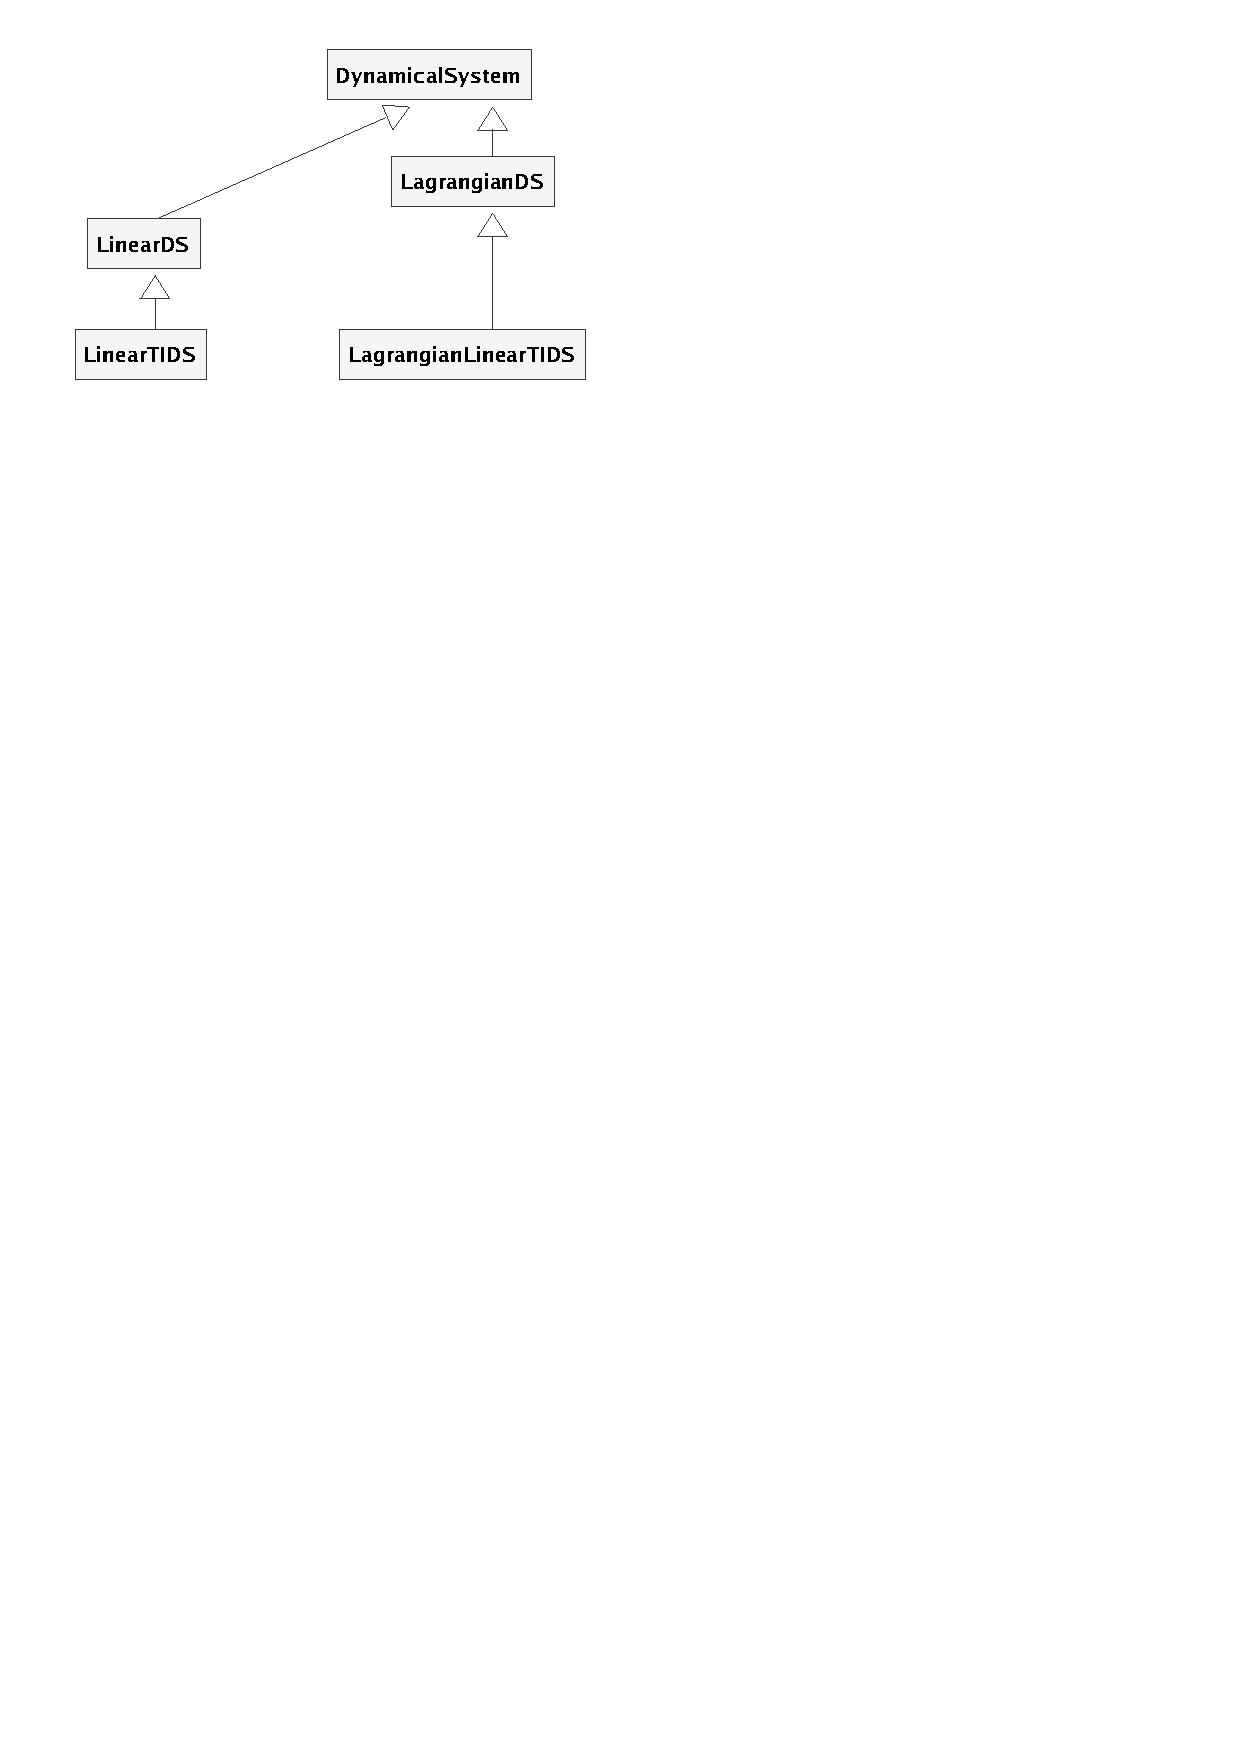
\includegraphics[width=0.3\textwidth]{./DSClassDiagram.pdf}
  \label{DSDiagram}
\end{figure}
% DYNAMICAL SYSTEMS
\section{General non linear first order dynamical systems \\ $\rightarrow$ class \it{DynamicalSystem}}
This is the top class for dynamical systems. All other systems classes derived from this one. \\

A general dynamical systems is described by the following set of $n$ equations, completed with initial conditions:
\begin{eqnarray}
  \dot x &=& f(x,t) + T(x) u(x, \dot x, t) + r \\
  x(t_0)&=&x_0 
\end{eqnarray}

\begin{itemize}
\item $x$: state of the system - Vector of size $n$.
\item $f(x,t)$: vector field - Vector of size $n$.
\item $u(x, \dot x, t)$: control term - Vector of size $uSize$.
\item $T(x)$: $n\times uSize$ matrix, related to control term.
\item $r$: input due to non-smooth behavior - Vector of size $n$.
\end{itemize}

The Jacobian matrix, $\nabla_x f(x,t)$, of $f$ according to $x$, $n\times n$ square matrix, is also a member of the class. \\

Initial conditions are given by the member $x_0$, vector of size $n$. This corresponds to x value when
simulation is starting, ie after a call to strategy->initialize(). \\

There are plug-in functions in this class for $f$ (vectorField), $jacobianX$, $u$ and $T$. All
of them can handle a vector of user-defined parameters. 

% LINEAR DS
\section{First order linear dynamical systems $\rightarrow$ class \it{LinearDS}}

Derived from DynamicalSystem, described by the set of $n$ equations and initial conditions: 
\begin{eqnarray}
  \dot x &=& A(t)x(t)+Tu(t)+b(t)+r \\
  x(t_0)&=&x_0 
\end{eqnarray}
With:
\begin{itemize}
\item $A(t)$: $n\times n$ matrix, state independent but possibly time-dependent.
\item $b(t)$: Vector of size $n$, possibly time-dependent.
\end{itemize}
Other variables are those of DynamicalSystem class. \\
$A$ and $B$ have corresponding plug-in functions. \\

Warning: time dependence for $A$ and $b$ is not available at the time in the simulation part for this kind of dynamical systems. \\

Links with vectorField and its Jacobian are: 
\begin{eqnarray}
  f(x,t) &=& A(t)x(t)+b(t) \\
  jacobianX&=&\nabla_x f(x,t) = A(t) 
\end{eqnarray}

% LAGRANGIANDS
\section{Second order non linear Lagrangian dynamical systems \\  $\rightarrow$ class \it{LagrangianDS}}

Lagrangian second order non linear systems are described by the following set of$nDof$ equations + initial conditions:
\begin{eqnarray}
 M(q) \ddot q + NNL(\dot q, q) + F_{Int}(\dot q , q , t) &=& F_{Ext}(t) + p \\
 q(t_0) &=& q0 \\
 \dot q(t_0) &=& velocity0 
\end{eqnarray}
With:
\begin{itemize}
\item $M(q)$: $nDof\times nDof$ matrix of inertia.
\item $q$: state of the system - Vector of size $nDof$.
\item $\dot q$ or $velocity$: derivative of the state according to time - Vector of size $nDof$.
\item $NNL(\dot q, q)$:  non linear terms, time-independent - Vector of size $nDof$.
\item $F_{Int}(\dot q , q , t)$: time-dependent linear terms - Vector of size $nDof$.
\item $F_{Ext}(t)$: external forces, time-dependent BUT do not depend on state - Vector of size $nDof$.
\item $p$: input due to non-smooth behavior - Vector of size $nDof$.
\end{itemize}

The following Jacobian are also member of this class:
\begin{itemize}
\item jacobianQFInt = $\nabla_q F_{Int}(t,q,\dot q)$ - $nDof\times nDof$ matrix.
\item jacobianVelocityFInt = $\nabla_{\dot q} F_{Int}(t,q,\dot q)$ - $nDof\times nDof$ matrix.
\item jacobianQNNL = $\nabla_q NNL(q,\dot q)$ - $nDof\times nDof$ matrix.
\item jacobianVelocityNNL = $\nabla_{\dot q}NNL(q,\dot q)$ - $nDof\times nDof$ matrix.
\end{itemize}


There are plug-in functions in this class for $F_{int}$, $F_{Ext}$, $M$, $NNL$ and the four Jacobian matrices. All
of them can handle a vector of user-defined parameters. \\

Links with first order dynamical system are: 
\begin{eqnarray}
  n &= &2nDof \\
  x &=&\left[\begin{array}{c}q \\ \dot q \end{array}\right] \\
  f(x,t) &=&  \left[\begin{array}{c} \dot q \\ M^{-1}(F_{Ext}-F_{Int}-NNL) \end{array}\right] \\
  \\
  \nabla_x f(x,t) &=& 
  \left[\begin{array}{cc} 
      0_{nDof\times nDof} & I_{nDof\times nDof} \\
      \nabla_q(M^{-1})(F_{Ext}-F_{Int}-NNL) -M^{-1}\nabla_q(F_{Int}+NNL) &  -M^{-1}\nabla_{\dot q}(F_{Int}+NNL) 
    \end{array}\right] \\
  r &=& \left[\begin{array}{c} 0_{nDof} \\ p \end{array}\right] \\
  u(x,\dot x,t) &=& u_L(\dot q, q, t) \text{  (not yet implemented)} \\
  T(x) &=& \left[\begin{array}{c} 0_{nDof} \\ T_L(q) \end{array}\right] \text{  (not yet implemented)} \\
\end{eqnarray}
With $0_{n}$ a vector of zero of size $n$, $0_{n\times m}$ a $n\times m$ zero matrix and
$I_{n\times n}$, identity $n\times n$ matrix. \\

Warning: control terms ($Tu$) are not fully implemented in Lagrangian systems. This will be part of future version.

% LAGRANGIAN LINEAR TIME INVARIANT DS
\section{Second order linear and time-invariant Lagrangian dynamical systems $\rightarrow$ class \it{LagrangianLinearTIDS}}
\label{Sec:LagrangianLineatTIDS}
\begin{eqnarray}
M \ddot q + C \dot q + K q =  F_{Ext}(t) + p
\end{eqnarray}

With:
\begin{itemize}
\item $C$: constant viscosity $nDof\times nDof$ matrix 
\item $K$: constant rigidity $nDof\times nDof$ matrix 
\end{itemize}

And: 
\begin{eqnarray}
F_{Int} &=& C \dot q + K q \\
NNL &=& 0_{nDof} 
\end{eqnarray}



\chapter{Dynamical Systems implementation in Siconos.}

\begin{table}[!ht]
  \begin{tabular}{|l|l|}
    \hline
    author  & F.  P\'erignon \\
    \hline
    date    & November 7, 2006 \\ 
    \hline
    version & Kernel 1.3.0 \\
    \hline
  \end{tabular}
\end{table}




\section{Introduction}
This document is only a sequel of notes and remarks on the way Dynamical Systems are implemented in Siconos.\\
It has to be completed, reviewed, reorganized etc etc for a future Developpers'Guide. \\
See also documentation in Doc/User/DynamicalSystemsInSiconos for a description of various dynamical systems types.

\section{Class Diagram}
There are four possible formulation for dynamical systems in Siconos,
two for first order systems and two for second order Lagrangian systems. The main class is DynamicalSystem, all other derived from this one, as shown in the following diagram:
\begin{figure}[htbp]
  \centering
 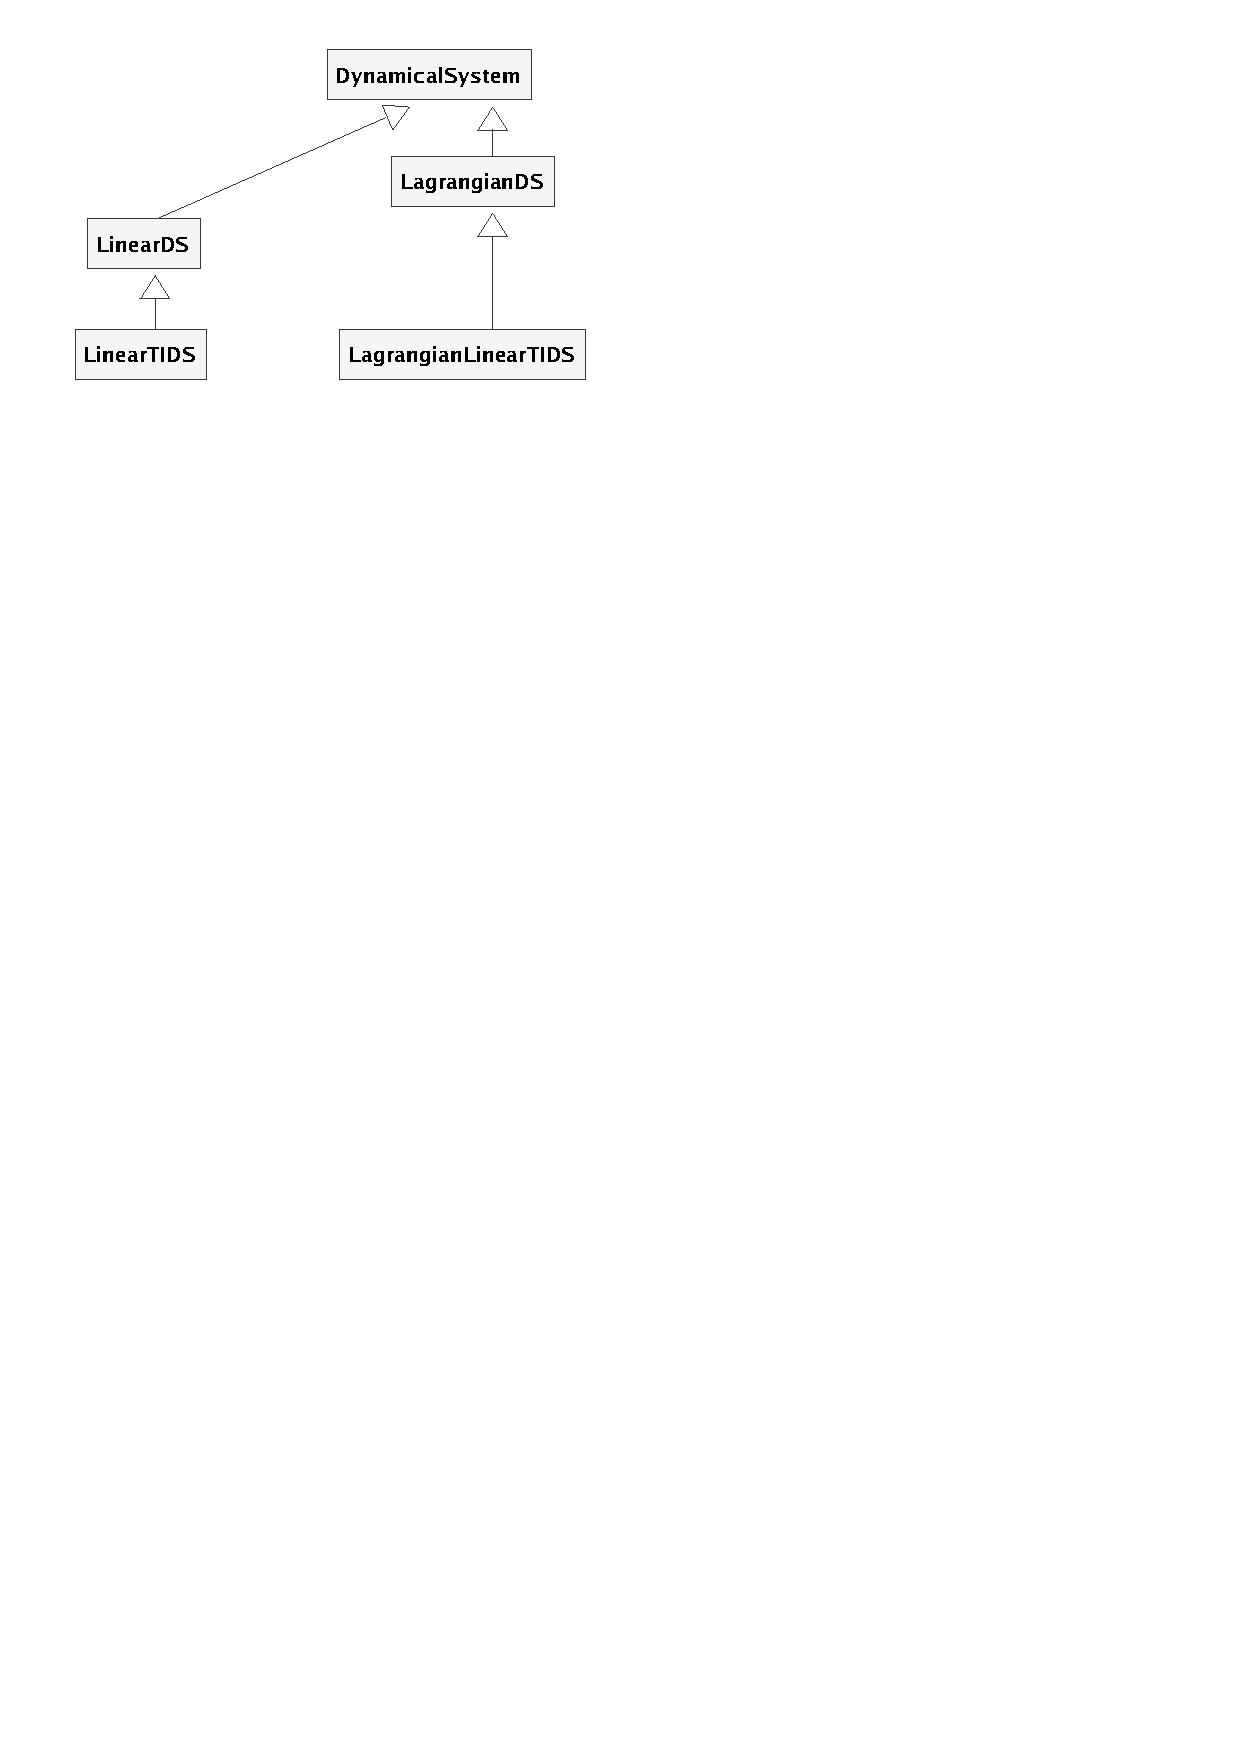
\includegraphics[width=0.3\textwidth]{./DSClassDiagram.pdf}
  \label{DSDiagram}
\end{figure}
% DYNAMICAL SYSTEMS

\section{Construction}

Each constructor must:
\begin{itemize}
\item initialize all the members of the class and of the top-class if it exists
\item allocate memory and set value for all required inputs
\item allocate memory and set value for optional input if they are given as argument (in xml for example)
\item check that given data are coherent and that the system is complete (for example, in the LagrangianDS
if the internal forces are given as a plug-in, their Jacobian are also required. If they are not given, this leads to an exception).
\end{itemize}

No memory allocation is made for unused members $\Rightarrow$ requires if statements in simulation.  (if!=NULL ...).\\

\subsection{DynamicalSystem}

{\bf Required data:}\\
n, x0, f, jacobianXF \\
{\bf Optional:}\\
T,u \\

\textbf{Always allocated in constructor:} \\
x, x0, xFree, r, rhs, jacobianXF

Warning: default constructor is always private or protected and apart from the others and previous rules or remarks do not always apply to it. 
This for DS class and any of the derived ones. 

\subsection{LagrangianDS}

\textbf{Required data:}\\
ndof, q0, velocity0, mass \\
\textbf{Optional:}\\
fInt and its Jacobian, fExt, NNL and its Jacobian. \\

\textbf{Always allocated in constructor:} \\
mass, q, q0, qFree, velocity, velocity0, velocityFree, p. \\
All other pointers to vectors/matrices are set to NULL by default. \\
Memory vectors are required but allocated during call to initMemory function. 

Various rules:
\begin{itemize}
\item fInt (NNL) given as a plug-in $\Rightarrow$ check that JacobianQ/Velocity are present (matrices or plug-in)
\item any of the four Jacobian present $\Rightarrow$ allocate memory for block-matrix jacobianX  (connectToDS function)
\item 
\end{itemize}

check: end of constructor or in initialize? \\
computeF and JacobianF + corresponding set functions: virtual or not? \\


\section{Specific flags or members}

\begin{itemize}
\item isAllocatedIn: to check inside-class memory allocation
\item isPlugin: to check if operators are computed with plug-in or just directly set as a matrix or vector
\item workMatrix: used to save some specific matrices in order to avoid recomputation if possible (inverse of mass ...)
\end{itemize}

\section{plug-in management}
DynamicalSystem class has a member named parameterList which is a $map<string, SimpleVector*>$, ie a list of
pointers to SimpleVector*, with a string as a key to identified them. 
For example, $parametersList["mass"]$ is a SimpleVector*, which corresponds to the last argument given in 
mass plug-in function. \\
By default, each parameters vectors must be initialized with a SimpleVector of size 1, as soon as the plug-in is
declared. Moreover, to each vector corresponds a flag in isAllocatedIn map, to check if the corresponding vector has been 
allocated inside the class or not. \\ 
For example, in DynamicalSystem, if $isPlugin["vectorField"]==true$, then, during call to constructor or set function,
it is necessary to defined the corresponding parameter: \\
$parametersList["vectorField"] = new SimpleVector(1)$ \\
and to complete the $isAllocatedIn$ flag: \\
$isAllocatedIn["parameter_for_vectorField"] = true$. \\

\chapter{Interactions}
\begin{table}[!ht]
  \begin{tabular}{|l|l|}
    \hline
    author  & F.  P\'erignon \\
    \hline
    date    & November 7, 2006 \\ 
    \hline
    version & Kernel 1.3.0 \\
    \hline
  \end{tabular}
\end{table}

\section{Introduction}
This document is only a sequel of notes and remarks on the way Interactions are implemented in Siconos.\\
It has to be completed, reviewed, reorganized etc etc for a future Developpers'Guide. \\
See also documentation in Doc/User/Interaction.

\section{Class Diagram}

\section{Description}

\begin{ndrfp} 
review of interactions (for EventDriven implementation) 17th May 2006.
\end{ndrfp}

\bei
\item variable \varcpp{nInter} renamed in \varcpp{interactionSize}: represents the size of \varcpp{y} and \varcpp{$\lambda$}. NOT the number of relations !! \\
\item add a variable \varcpp{nsLawSize} that depends on the non-smooth law type.\\
Examples:
\bei
\item NewtonImpact -> \varcpp{nsLawSize} = 1
\item Friction 2D  -> \varcpp{nsLawSize} = 2
\item Friction 3D  -> \varcpp{nsLawSize} = 3
\item ... 
\item \varcpp{nsLawSize} = n with n dim of matrix D in :
$y=Cx+D\lambda$, D supposed to be a full-ranked matrix. \\
Warning: this case is represented by only one relation of size n. 
\ei
\item \varcpp{numberOfRelations}: number of relations in the interaction, \varcpp{numberOfRelations} = $\Frac{\varcpp{interactionSize}}{\varcpp{nsLawSize}}$.
\ei


\chapter{Notes on the Non Smooth Dynamical System construction}
\begin{table}[!ht]
  \begin{tabular}{|l|l|}
    \hline
    author  & F.  P\'erignon \\
    \hline
    date    & November 7, 2006 \\ 
    \hline
    version & Kernel 1.3.0 \\
    \hline
  \end{tabular}
\end{table}

\section{Introduction}

\section{Class Diagram}

\section{Description}

Objects must be constructed in the following order: 
\bei
\item DynamicalSystems
\item NonSmoothLaw: depends on nothing
\item Relation: no link with an interaction during construction, this will be done during initialization. 
\item Interaction: default constructor is private and copy is forbidden. Two constructors: xml and from data. Required data are a DSSet, a NonSmoothLaw and
a Relation (+ dim of the Interaction and a number). \\
Interaction has an initialize function which allocates memory for y and lambda, links correctly the relation and initializes it .... This function is called at the 
end of the constructor. That may be better to call it in simulation->initialize? Pb: xml constructor needs memory allocation for y and lambda if they are
provided in the input xml file. 
\item NonSmoothDynamicalSystem: default is private, copy fobidden. Two constructors: xml and from data. Required data are the DSSet and the InteractionsSet.
The topology is declared and constructed (but empty) during constructor call of the nsds, but initialize in the Simulation, this because it can not be initialize until the nsds has been fully described (ie this to allow user to add DS, Inter ...) at any time in the model, but before simulation initialization). 

\ei

\section{misc}

\bei 
\item no need to keep a number for Interactions? Only used in xml for OSI, to know which Interactions it holds.
\item pb: the number of saved derivatives for y and lambda in Interactions is set to 2. This must depends on the relative degree which is computes during
Simulation initialize and thus too late. It is so not available when memory is allocated (Interaction construction). Problem-> to be reviewed.
\ei 


\chapter{OneStepIntegrator and derived classes.}
\begin{table}[!ht]
  \begin{tabular}{|l|l|}
    \hline
    author  & F.  P\'erignon \\
    \hline
    date    & November 7, 2006 \\ 
    \hline
    version & Kernel 1.3.0 \\
    \hline
  \end{tabular}
\end{table}

\section{Introduction}
This document is only a sequel of notes and remarks on the way OneStepIntegrators are implemented in Siconos.\\
It has to be completed, reviewed, reorganized etc etc for a future Developpers'Guide. \\
See also documentation in Doc/User/OneStepIntegrator for a description of various OSI.

\section{Class Diagram}

\section{Misc}

OSI review for consistency between Lsodar and Moreau:
\begin{itemize}
\item add set of DynamicalSystem*
\item add set of Interaction* 
\item add link to strategy that owns the OSI
\item remove td object in OSI -> future: replace it by a set of td (one per ds)
\item add strat in constructors arg list
\end{itemize}



osi -> strat -> Model -> nsds -> topology \\
osi -> strat -> timeDiscretisation \\

let a timeDiscretisation object in the OSI? set of td (one per ds)? \\
create a class of object that corresponds to DS on the simulation side ? \\
will contain the DS, its discretization, theta for Moreau ... ? \\ 
Allow setStrategyPtr operation? Warning: need reinitialisation. \\


Required input by user: \\
\begin{itemize}
\item list of DS or list of Interactions ? 
\item pointer to strategy
\item ...
\end{itemize}

\section{Construction}

Each constructor must:

\begin{itemize}
\item
\end{itemize}

\subsection{Moreau}

Two maps: one for W, and one for theta. To each DS corresponds a theta and a W. \\
Strategy arg in each constructor.

\textbf{Required data:}\\

\textbf{Optional:}\\

\textbf{Always allocated in constructor:} \\

Warning: default constructor is always private or protected and apart from the others and previous rules or remarks do not always apply to it. 

\subsection{Lsodar}

\textbf{Required data:}\\

\textbf{Optional:}\\

\textbf{Always allocated in constructor:} \\

\chapter{First Order Nonlinear Relation }

\begin{table}[!ht]
  \begin{tabular}{|l|l|}
    \hline
    author  & 0. Bonnefon \\
    \hline
    date    & July, 1 2009 \\ 
    \hline
    version & Kernel 3.0.0 \\
    \hline
  \end{tabular}
\end{table}

\chapter{Computation of the number of Index Set and various levels}
\begin{table}[!ht]
  \begin{tabular}{|l|l|}
    \hline
    author  & V. Acary \\
    \hline
    date    & Septembre 16, 2011 \\ 
    \hline
    version & Kernel 3.3.0 \\
    \hline
  \end{tabular}
\end{table}


In this chapter, we give some hints on the automatic computation of the number of index sets, the number of derivatives in the {\tt Interaction} and the levelMin and LevelMax.


\section{Why is the  relative degree not relevant ?}
In this section, we give a very brief overview of the notion of relative degree.

\subsection{First order Linear complementary systems}

 A  Linear Complementarity System (LCS) is defined by
\begin{equation}
  \label{eq:LCS-bis}
  \begin{cases}
    \dot x = A x +B \lambda \\
     y = C x + D \lambda\\
    0 \leq  y \perp \lambda \geq 0 \\
  \end{cases}
\end{equation} 
 \begin{definition}[Relative degree in the SISO case]
      Let us consider a linear system in state representation given by the quadruplet $(A,B,C,D) \in \RR^{n\times n}\times\RR^{n \times m}\times \RR^{m\times n}\times\RR^{m\times m} $:
      \begin{equation}
        \label{eq:LS}
        \begin{cases}
          \dot x = A x +B \lambda \\
          y = C x + D \lambda
        \end{cases}
      \end{equation}
      \begin{itemize}
      \item In the Single Input/ Single Output (SISO) case ($m=1$), the relative
        degree is defined by the first non zero Markov parameters :
        \begin{equation}
          \label{eq:Markov-Parameter}
          D, CB, CAB, CA^2B, \ldots, CA^{r-1}B, \ldots
        \end{equation}
      \item In the multiple input/multiple output (MIMO) case ($m>1$), an \textit{uniform} relative degree is defined as follows.
        If $D$ is non singular, the relative degree is equal to $0$. Otherwise, it is assumed to be the first positive integer $r$ such that 
        \begin{equation}
          \label{eq:mimo-r}
          CA^{i}B =0, \quad i=0\ldots q-2
        \end{equation}
        while
        \begin{equation}
          \label{eq:mimo-r2}
          CA^{r-1}B \text{ is non singular}.
        \end{equation}
      \end{itemize}
    \end{definition}
    The Markov parameters arise naturally when we derive with respect
    to time the output $y$,
    \begin{eqnarray*}
      \label{eq:y-derive}
      y &=& C x + D \lambda \\
      \dot y &=& CA x + CB \lambda, \text{ if } D= 0  \\
      \ddot y &=& CA^2 x + CAB \lambda, \text{ if }  D=0, CB=0\\
      &\ldots& \\
      y^{(r)} &=& CA^{r} x + CA^{r-1}B \lambda, \text{ if } D=0, CB=0, CA^{r-2}B=0, r=1\ldots r-2 \\
      &\ldots&
    \end{eqnarray*}
    and the first non zero Markov parameter allows us to define the
    output $y$ directly in terms of the input $\lambda$.

In continuous time, the nature of solutions depends strongly on the relative degree. When we want to perform the time--integration of such systems, we need also to reduce the relative degree or to known it to correctly operate.

We can observe that the relative degree $0$ is well defined only by the relation ($D$ nonsingular) and by the nonsmooth law. Indeed, let us imagine that the nonsmooth law is defined by $0\leq\dot y \perp \lambda \geq 0 $. We can easily see that the relative degree is reduced.

In the MIMO, the computation of non uniform relative degree is hard task. This is also the case for nonlinear systems.



\subsection{Second order Lagrangian systems}


Let us consider a second order linear and time-invariant Lagrangian dynamical system (see \S~\ref{Sec:LagrangianLineatTIDS})
\begin{equation}
  \label{eq:rd1}
  \begin{cases}
    M \dot v + C v + K q = F_{Ext}(t) + p \\
    \dot q = v
  \end{cases}
\end{equation}
together with a Lagrangian linear relation
\begin{equation}
  y= Cq + e + D \lambda + Fz,
  \label{eq:rd2}
\end{equation}
\begin{equation}
  p = C^t \lambda
\label{eq:rd3}  
\end{equation}
and a simple nonsmooth law,
\begin{equation}
  0\leq y \perp \lambda \geq 0
\label{eq:rd4}  
\end{equation}

If $D>0$, the relative degree is uniformly zero and the system can be solved without deriving the output~(\ref{eq:rd2}). Indeed, we known that the solution of the LCP
\begin{equation}
  0\leq Cq + e + D \lambda + Fz, \perp \lambda \geq 0
\label{eq:rd5}  
\end{equation}
is unique and Lipschitz with respect to $q$. It can be denoted as $\lambda(q) = \mbox{SOL}(D,Cq + e +Fz)$. Therefore, the differential equation~(\ref{eq:rd1}) reduces to a standard ODE with a Lipschitz RHS
 \begin{equation}
  \label{eq:rd6}
  \begin{cases}
    M \dot v + C v + K q = F_{Ext}(t) + C^t \lambda(q)  \\
    \dot q = v
  \end{cases}
\end{equation}

In the case that we deal with unilateral contact, we usually have $D=0$ and the relative degree of the system is $2$. In this case, the output has to be differentiated as
\begin{equation}
  \label{eq:rd7}
   \dot y= C \dot q,
\end{equation}
and an impact law has to added, for instance the newton's impact law
\begin{equation}
  \label{eq:rd8}
  \text{ if } y=0, \text{ when } \dot y^+= -e y^-
\end{equation}
In the same vein, the equations of motion (\ref{eq:rd1}) is not sufficient since the velocity may encounter jumps. The dynamics is usually replaced by a measure differential equation of the form
\begin{equation}
  \label{eq:rd10}
  \begin{cases}
    M dv + C v^+(t) dt + K q(t) dt = F_{Ext}(t)dt + di \\
    \dot q = v
  \end{cases}
\end{equation}
where $di$ is the measure that can be related to $p$ thanks to
\begin{equation}
  \label{eq:rd11}
  di = p dt + \sigma \delta _{t^*}
\end{equation}
is only one jump is expected at ${t^*}$.


\subsection{Conclusion for the implementation}
From the continuous time mathematical analysis, the relative degree is very important to know if we have to compute the derivatives of the output $y^{(n)}$ and to consider various levels for the input $p , \sigma, ....$

However in the numerical practice,  the time --discretization makes an assumption on the relative degree and treats the nonsmooth law at different levels. The resulting time discretized system posseses more or less variables.

Consider for instance  (\ref{eq:rd1}) in the case of the Moreau scheme
\begin{subnumcases}{\label{eq:MoreauTS}}
  M(v_{k+1}-v_k)  + h  (K q_{k+\theta}+ C v_{k+\theta}) = p_{k+1} = G(q_{k+1}) \lambda_{k+1},\quad\,\\[1mm] 
  q_{k+1} = q_{k} + h v_{k+\theta}, \quad \\[1mm]
  \dot y_{k+1} = G^\top(q_{k+1})\, v_{k+1} \\[1mm]
  \begin{array}{l}
    \text{if }\quad\bar y^\alpha_{k+1} \leq 0 \text{ then } 0 \leq \dot y^\alpha_{k+1} + e  \dot y^\alpha_{k} \perp \lambda^\alpha_{k+1}  \geq 0, \\[1mm]
    \text{otherwise  } \lambda^\alpha_{k+1}  =0.\label{eq:MoreauTSd}
  \end{array}, \alpha \in \mathcal I
\end{subnumcases} 
and the Schatzman--Paoli  scheme
\begin{subnumcases}{}
  M(q_{k+1}-2q_{k}+q_{k-1})  + h^2 (K q_{k+\theta}+ C v_{k+\theta})  =  p_{k+1},\quad\,\\ \notag\\ 
  v_{k+1}=\Frac{q_{k+1}-q_{k-1}}{2h}, \\ \notag \\
  y_{k+1} = h\left(\Frac{q_{k+1}+e q_{k-1}}{1+e}\right) \\
  p_{k+1}= G\left(\Frac{q_{k+1}+e q_{k-1}}{1+e}\right) \lambda_{k+1} \\
  0 \leq y_{k+1}  \perp\lambda_{k+1} \geq 0 .
\end{subnumcases}

We can see easily that the number of derivatives (or levels) that we store for $y$ and $\lambda$ is independent on the relative degree but is chosen by the {\tt OneStepIntegrator} with respect to the type of systems.

\section{How to define and compute the various levels and the number of indexSets }

\subsection{$y$ related variables}

The size of the vector {\tt y} in the {\tt Interaction} depends on
\begin{itemize}
\item the {\tt  OneStepIntegrator} type.
  \begin{itemize}
  \item see the difference between the Moreau and Schatzman Paoli
    scheme,
  \item plan the time--discontinuous Galerkin scheme
  \item plan the Higher Order Moreau sweeping process (HOSP)
  \end{itemize}
\item the {\tt  Simulation} type.
  \begin{itemize}
  \item In {\tt Timestepping} or {\tt Event-driven} we do not need the same number of stored $y$
  \end{itemize}

\item the {\tt NonSmoothLaw} type.
  \begin{itemize}
  \item If we consider some cases with or without friction in {\tt
      Timestepping} or {\tt Event-driven}, we need to adapt the number
    of stored $y$
  \end{itemize}

\end{itemize}

Since the various levels of  {\tt y} are used to build the index sets we will need from $0$ to a computed size that depends on the previous criteria. Only a part will be used in the {\tt OneStepNSProblem}.

\subsection{$\lambda$ related variables}

The size of the vector {\tt lambda} in the {\tt Interaction} depends on the same criteria than in the previous section.  Only, the number of lambda is not the same as {\tt y} since a multiplier {\tt lambda[i]} is not necessarily related to {\tt y[i]}

\section{Rules for implementation}

We can define new members in {\tt Interaction}:
\begin{itemize}
\item {\tt \_lowerlevelForOutput}, this value is to $0$ by default
\item {\tt \_upperlevelForOutput},  this value must be computed at initialization with respect to the previous criteria
\item {\tt \_lowerlevelForInput},  this value must be computed at initialization with respect to the previous criteria
\item {\tt \_upperlevelForInput},  this value must be computed at initialization with respect to the previous criteria
\end{itemize}




This level are computed in {\tt Simulation::ComputeLevelsForInputAndOutput}. A visitor is used for the {\tt OneStepIntegrator}. Furthermore, four global levels are computed 
\begin{itemize}
\item {\_levelMinForOutput} this value is the minimum level for the output {\tt Interaction::\_lowerlevelForOutput}  for all the interactions
\item {\_levelMaxForOutput} this value is the maximum level for the output {\tt Interaction::\_upperlevelForOutput}  for all the interactions
\item {\_levelMinForInput} this value is the minimum level for the output {\tt Interaction::\_lowerlevelForInput}  for all the interactions
\item {\_levelMaxForInput} this value is the maximum level for the output {\tt Interaction::\_upperlevelForInput}  for all the interactions
\end{itemize}




\begin{itemize}
\item the values {\tt y[i]} must be initialized from {\tt \_lowerlevelForOutput} to {\tt \_upperlevelForOutput}.
\item the values {\tt lamdba[i]} must be initialized from {\tt \_lowerlevelForInput} to  {\tt \_upperlevelForInput}.
\item the values {\tt y[i]} in {\tt Interaction} must be used in priority to store the i-th derivative of $y$. When it is needed, higher index $i$ can be used for other triggering variables. For instance, for an Event--Driven scheme with a Lagrangian systems with friction, sliding velocity must be stored.
\item the values of {\tt lamdba[i]} must stored the various multiplier for the nonsmooth law. We affect the same index $i$ as for the level of {\tt y[i]} present in the corresponding nonsmooth law.
\item The number of {\tt IndexSets} should follows {\tt \_levelMaxForY}.
\end{itemize}



For the dynamical systems :
\begin{itemize}
\item The number of levels for {\tt \_r} and {\tt \_p} in the DS should follow {\tt \_lowerlevelForInput} and {\tt \_upperlevelForOutput} of the associated interactions. This is done in {\tt Interaction::initialize}.
\item A new variable should be added in the LagrangianDS to store the multiplier at the position level ({\tt \_tau} ?) to avoid the use of {\tt \_p[0]}. Indeed, we will continue to assume that {\tt \_p} is the input in the equation of motion. For {\tt lambda} we can  use {\tt lambda[0]} 
\end{itemize}

TODO LIST AND QUESTIONS
\begin{itemize}
\item What about the case of multiples interactions on a DS with various {\tt \_lowerlevelForInput} and {\tt \_upperlevelForOutput} ? Normally, all the levels should be correctly initialized thanks to the proposed implementation (r2821)
\item {\tt DynamicalSystem::\_r} should be a VectorOfVectors
\item {\tt DynamicalSystem::\_r} is split in {\tt LagrangianDS}. a first part is {\tt LagrangianDS::\_p}. The other is not implemented !! {\tt LagrangianDS::\_tau} ?
\end{itemize}


%%% Local Variables: 
%%% mode: latex
%%% TeX-master: "DevNotes"
%%% End: 



\chapter{Newton's linearization for First Order Systems}
 \begin{table}[!ht]
  \begin{tabular}{|l|l|}
    \hline
    author  & O.Bonnefon, V. Acary\\
    \hline
    date    & Sept, 07, 2007 \\ 
    last update        & Feb, 2011 \\
                       & April, 2014 \\
    \hline
    version &  \\
    \hline
  \end{tabular}
\end{table}



This section is devoted to the implementation and the study  of the algorithm. The interval of integration is $[0,T]$, $T>0$, and a grid $t_{0}=0$, $t_{k+1}=t_{k}+h$, $k \geq 0$, $t_{N}=T$ is constructed. The approximation of a function $f(\cdot)$ on $[0,T]$ is denoted as $f^{N}(\cdot)$, and is a piecewise constant function, constant on the intervals $[t_{k},t_{k+1})$. We denote $f^{N}(t_{k})$ as $f_{k}$. The time-step is $h>0$. 


\section{Various first order dynamical systems with input/output relations}

\paragraph{FirstOrderR. Fully nonlinear case}
Let us introduce the following system, 
\begin{equation}
\begin{array}{l}
M \dot{x}(t) = f(x(t),t) + r(t)  \\[2mm]
y(t) = h(t,x(t),\lambda (t)) \\[2mm]
r(t) = g(t,x(t),\lambda (t) ) \\[2mm]
\end{array}
\label{first-DS}
\end{equation}
where $\lambda(t) \in \RR^m$  and $y(t) \in \RR^m$ are  complementary variables related through a multi-valued mapping.   According to the class of systems, we are studying, the function $f$ and $g$ are defined by a fully nonlinear framework or by affine functions. We have decided to present the time-discretization in its full generality and specialize the algorithms for each cases in Section~\ref{Sec:Spec}. This fully nonlinear case is not  implemented in Siconos yet. This fully general case is not yet implemented in Siconos.

This case is implemented in Siconos with the relation {\tt FirstOrderR} using the subtype {NonLinearR}

\paragraph{FirstOrderType1R}
Let us introduce a new notation,
\begin{equation}
\begin{array}{l}
M \dot{x}(t) = f(x(t),t) + r(t)  \\[2mm]
y(t) = h(t,x(t)) \\[2mm]
r(t) = g(t,\lambda (t) ) \\[2mm]
\end{array}
\label{first-DS1}
\end{equation}
This case is implemented in Siconos with the relation {\tt FirstOrderType1R}.



\paragraph{FirstOrderType2R}
Let us introduce a new notation, 
\begin{equation}
\begin{array}{l}
M \dot{x}(t) = f(x(t),t) + r(t)  \\[2mm]
y(t) = h(t,x(t),\lambda (t)) \\[2mm]
r(t) = g(t,\lambda (t) ) \\[2mm]
\end{array}
\label{first-DS2}
\end{equation}
This case is implemented in Siconos with the relation {\tt FirstOrderType2R}.




\paragraph{Linear case }Let us introduce a new notation, 
\begin{equation}
\begin{array}{l}
M \dot{x}(t) = Ax(t) + r(t)  +b(t)\\[2mm]
y(t) = h(x(t),\lambda (t),z) = Cx + Fz + D \lambda  \\[2mm]
r(t) = g(t,\lambda (t) ) = B \lambda \\[2mm]
\end{array}
\label{first-DS3}
\end{equation}


\section{Time--discretizations}



\subsection{Standard $\theta-\gamma$ scheme.}
Let us now proceed with the time discretization of (\ref{first-DS3}) by a fully implicit scheme : 
\begin{equation}
  \begin{array}{l}
    \label{eq:toto1}
     M x_{k+1} = M x_{k} +h\theta f(x_{k+1},t_{k+1})+h(1-\theta) f(x_k,t_k) + h \gamma r(t_{k+1})
     + h(1-\gamma)r(t_k)  \\[2mm]
     y_{k+1} =  h(t_{k+1},x_{k+1},\lambda_{k+1}) \\[2mm]
     r_{k+1} =  g(t_{k+1},x_{k+1},\lambda_{k+1})\\[2mm]
     \mbox{NsLaw} ( y_{k+1} , \lambda_{k+1})
  \end{array}
\end{equation}
where $\theta = [0,1]$ and $\gamma \in [0,1]$. As in \cite{acary2008}, we call the problem \eqref{eq:toto1} the ``one--step nonsmooth problem''.

In the Siconos/Kernel module, the use of $\gamma$  is activated in the class {\tt EulerMoreauOSI} by the boolean {\tt \_useGamma}.



 This time-discretization is slightly more general than a standard implicit Euler scheme. The main discrepancy lies in the choice of a $\theta$-method to integrate the nonlinear term. For $\theta=0$, we retrieve the explicit integration of the smooth and  single valued term $f$. Moreover for $\gamma =0$, the term $g$ is explicitly evaluated. The flexibility in the choice of $\theta$ and $\gamma$ allows the user to improve and control the accuracy, the stability and the numerical damping of the proposed method. For instance, if the smooth dynamics given by $f$ is stiff, or if we have to use big step sizes for practical reasons, the choice of $\theta > 1/2$ offers better stability with the respect to $h$.

\subsection{Full $\theta-\gamma$ scheme}

Another possible time--discretization is as follows.
\begin{equation}
  \begin{array}{l}
    \label{eq:toto1-ter}
    M x_{k+1} = M x_{k} + h\theta f(x_{k+1},t_{k+1})+h(1-\theta) f(x_k,t_k) + h r(t_{k+\gamma}) \\[2mm]
    y_{k+\gamma} = h(t_{k+\gamma},x_{k+\gamma},\lambda _{k+\gamma}) \\[2mm]
    r_{k+\gamma} = g(t_{k+\gamma},x_{k+\gamma},\lambda _{k+\gamma})\\[2mm]
    \mbox{NsLaw} ( y_{k+\gamma} , \lambda_{k+\gamma})
  \end{array}
\end{equation}
We call the scheme~(\ref{eq:toto1-ter}) the full $\theta-\gamma$ scheme since it uses also the evaluation at $t_{k+\gamma}$ for the relation.

In the Siconos/Kernel module, the time--stepping scheme is activated in the class {\tt EulerMoreauOSI} by the boolean {\tt \_useGammaForRelation}.


Another possibility for the time discretization in the nonlinear case would be
\begin{equation}
  \begin{array}{l}
    \label{eq:toto1-quat}
    M x_{k+1} = M x_{k} +h f(x_{k+\theta},t_{k+\theta}) + h r(t_{k+\gamma}) \\[2mm]
    y_{k+\gamma} =  h(t_{k+\gamma},x_{k+\gamma},\lambda _{k+\gamma}) \\[2mm]
    r_{k+\gamma} = g(t_{k+\gamma},x_{k+\gamma},\lambda _{k+\gamma})\\[2mm]
    \mbox{NsLaw} ( y_{k+\gamma} , \lambda_{k+\gamma})
  \end{array}
\end{equation}
This scheme has not been yet implemented in Siconos/Kernel.

\clearpage
\section{Newton's linearization of~(\ref{eq:toto1})} 

Due to the fact that  two of the  studied classes of systems that are studied in this paper are affine functions in terms of $f$ and $g$, we propose to solve the "one--step nonsmooth problem'' (\ref{eq:toto1}) by performing an external Newton linearization.

 \paragraph{Newton's linearization of the first line of~(\ref{eq:toto1})} The first line of the  problem~(\ref{eq:toto1}) can be written under the form of a residue $\mathcal R$ depending only on $x_{k+1}$ and $r_{k+1}$ such that 
\begin{equation}
  \label{eq:NL3}
  \mathcal R (x_{k+1},r _{k+1}) =0
\end{equation}
with 
\begin{equation}
\mathcal R(x,r) = M(x - x_{k}) -h\theta f( x , t_{k+1}) - h(1-\theta)f(x_k,t_k) - h\gamma r
- h(1-\gamma)r_k.
\end{equation}
The solution of this system of nonlinear equations is sought as a limit of the sequence $\{ x^{\alpha}_{k+1},r^{\alpha}_{k+1} \}_{\alpha \in \NN}$ such that
 \begin{equation}
   \label{eq:NL7}
   \begin{cases}
     x^{0}_{k+1} = x_k \\ \\
     r^{0}_{k+1} = r_k \\ \\
     \mathcal R_L( x^{\alpha+1}_{k+1},r^{\alpha+1}_{k+1}) = \mathcal
     R(x^{\alpha}_{k+1},r^{\alpha}_{k+1})  + \left[ \nabla_{x} \mathcal
     R(x^{\alpha}_{k+1},r^{\alpha}_{k+1})\right] (x^{\alpha+1}_{k+1}-x^{\alpha}_{k+1} ) +
     \left[ \nabla_{r} \mathcal R(x^{\alpha}_{k+1},r^{\alpha}_{k+1})\right] (r^{\alpha+1}_{k+1} - r^{\alpha}_{k+1} ) =0
 \end{cases}
\end{equation}
\begin{ndrva}
  What about $r^0_{k+1}$ ?
\end{ndrva}

The residu \free $\mathcal R _{\free}$ is also defined (useful for implementation only):
\[\mathcal R _{\free}(x) \stackrel{\Delta}{=}  M(x - x_{k}) -h\theta f( x , t_{k+1}) - h(1-\theta)f(x_k,t_k),\]
which yields
\[\mathcal R (x,r) = \mathcal R _{\free}(x)   - h\gamma r - h(1-\gamma)r_k.\]

\begin{equation}
  \mathcal R (x^{\alpha}_{k+1},r^{\alpha}_{k+1}) = \fbox{$\mathcal R^{\alpha}_{k+1} \stackrel{\Delta}{=}  \mathcal R
_{\free}(x^{\alpha}_{k+1})  - h\gamma r^{\alpha}_{k+1} - h(1-\gamma)r_k$}\label{eq:rfree-1}
\end{equation}

\[  \mathcal R
_{\free}(x^{\alpha}_{k+1},r^{\alpha}_{k+1} )=\fbox{$ \mathcal R _{\free, k+1} ^{\alpha} \stackrel{\Delta}{=}  M(x^{\alpha}_{k+1} - x_{k}) -h\theta f( x^{\alpha}_{k+1} , t_{k+1}) - h(1-\theta)f(x_k,t_k)$}\]
 
The computation of the Jacobian of $\mathcal R$ with respect to $x$, denoted by $   W^{\alpha}_{k+1}$ leads to 
\begin{equation}
   \label{eq:NL9}
   \begin{array}{l}
    W^{\alpha}_{k+1} \stackrel{\Delta}{=} \nabla_{x} \mathcal R (x^{\alpha}_{k+1},r^{\alpha}_{k+1})= M - h  \theta \nabla_{x} f(  x^{\alpha}_{k+1}, t_{k+1} ).\\
 \end{array}
\end{equation}
At each time--step, we have to solve the following linearized problem,
\begin{equation}
   \label{eq:NL10}
    \mathcal R^{\alpha}_{k+1} + W^{\alpha}_{k+1} (x^{\alpha+1}_{k+1} -
    x^{\alpha}_{k+1}) - h \gamma (r^{\alpha+1}_{k+1} - r^{\alpha}_{k+1} )  =0 ,
\end{equation}
By using (\ref{eq:rfree-1}), we get
\begin{equation}
  \label{eq:rfree-2}
  \mathcal R
_{\free}(x^{\alpha}_{k+1},r^{\alpha}_{k+1} )  - h\gamma r^{\alpha+1}_{k+1} - h(1-\gamma)r_k  + W^{\alpha}_{k+1} (x^{\alpha+1}_{k+1} -
    x^{\alpha}_{k+1})  =0 
\end{equation}

%\fbox
{
  \begin{equation}
    \label{eq:rfree-11}
    \boxed{ x^{\alpha+1}_{k+1} = h\gamma (W^{\alpha}_{k+1})^{-1}r^{\alpha+1}_{k+1} +x^\alpha_{\free}}
  \end{equation}
}
with :
\begin{equation}
  \label{eq:rfree-12}
  \boxed{x^\alpha_{\free}\stackrel{\Delta}{=}x^{\alpha}_{k+1}-(W^{\alpha}_{k+1})^{-1}\mathcal (R_{\free,k+1}^{\alpha} \textcolor{red}{- h(1-\gamma) r_k})}
\end{equation}

The matrix $W$ is clearly non singular for small $h$.




% that is

% \begin{equation}
%    \begin{array}{l}
%  h \gamma  r^{\alpha+1}_{k+1} = r_c + W^{\alpha}_{k+1} x^{\alpha+1}_{k+1}
%  .\label{eq:NL11} 
%  \end{array}
% \end{equation}
% with 
% \begin{equation}
%    \begin{array}{l}
% r_c \stackrel{\Delta}{=} h \gamma r^{\alpha}_{k+1} - W^{\alpha}_{k+1} x^{\alpha}_{k+1} + \mathcal R
% ^{\alpha}_{k+1}=- W^{\alpha}_{k+1} x^{\alpha}_{k+1} + \mathcal R_{\free k+1} ^{\alpha} - h(1-\gamma)r_k\\ \\
% \end{array}
% \end{equation}
% \begin{equation}
%    \begin{array}{l}
% \mathcal R ^{\alpha}_{k+1}=M( x^{\alpha}_{k+1} - x_k) -h \theta f(x^{\alpha}_{k+1})-h(1-\theta)f(x_k)
% - h \gamma r^{\alpha}_{k+1} -h(1- \gamma)r_k
%  \end{array}
%    \end{equation}
% \[x^{\alpha+1}_{k+1} = h(W^{\alpha}_{k+1})^{-1}r^{\alpha+1}_{k+1} +(W^{\alpha}_{k+1})^{-1}(\mathcal
% R_{\free k+1} ^{\alpha})+x^{\alpha}_{k+1}\]

 \paragraph{Newton's linearization of the second  line of~(\ref{eq:toto1})}
The same operation is performed with the second equation of (\ref{eq:toto1})
\begin{equation}
  \begin{array}{l}
    \mathcal R_y(x,y,\lambda)=y-h(t_{k+1},x,\lambda) =0\\ \\
  \end{array}
\end{equation}
which is linearized as
\begin{equation}
  \label{eq:NL9}
  \begin{array}{l}
    \mathcal R_{Ly}(x^{\alpha+1}_{k+1},y^{\alpha+1}_{k+1},\lambda^{\alpha+1}_{k+1}) = \mathcal
    R_{y}(x^{\alpha}_{k+1},y^{\alpha}_{k+1},\lambda^{\alpha}_{k+1}) +
    (y^{\alpha+1}_{k+1}-y^{\alpha}_{k+1})- \\[2mm] \qquad  \qquad \qquad \qquad  \qquad \qquad
    C^{\alpha}_{k+1}(x^{\alpha+1}_{k+1}-x^{\alpha}_{k+1}) - D^{\alpha}_{k+1}(\lambda^{\alpha+1}_{k+1}-\lambda^{\alpha}_{k+1})=0
  \end{array}
\end{equation}

This leads to the following linear equation
\begin{equation}
  \boxed{y^{\alpha+1}_{k+1} =  y^{\alpha}_{k+1}
  -\mathcal R^{\alpha}_{yk+1}+ \\
  C^{\alpha}_{k+1}(x^{\alpha+1}_{k+1}-x^{\alpha}_{k+1}) +
  D^{\alpha}_{k+1}(\lambda^{\alpha+1}_{k+1}-\lambda^{\alpha}_{k+1})}. \label{eq:NL11y}
\end{equation}
with,
\begin{equation}
     \begin{array}{l}
  C^{\alpha}_{k+1} = \nabla_xh(t_{k+1}, x^{\alpha}_{k+1},\lambda^{\alpha}_{k+1} ) \\ \\
  D^{\alpha}_{k+1} = \nabla_{\lambda}h(t_{k+1}, x^{\alpha}_{k+1},\lambda^{\alpha}_{k+1})
 \end{array}
\end{equation}
and
\begin{equation}\fbox{$
\mathcal R^{\alpha}_{yk+1} \stackrel{\Delta}{=} y^{\alpha}_{k+1} - h(x^{\alpha}_{k+1},\lambda^{\alpha}_{k+1})$}
 \end{equation}
 \paragraph{Newton's linearization of the third  line of~(\ref{eq:toto1})}
The same operation is performed with the third equation of (\ref{eq:toto1})
\begin{equation}
  \begin{array}{l}
    \mathcal R_r(r,x,\lambda)=r-g(t_{k+1},x,\lambda) =0\\ \\  \end{array}
\end{equation}
which is linearized as
\begin{equation}
  \label{eq:NL9}
  \begin{array}{l}
      \mathcal R_{Lr}(r^{\alpha+1}_{k+1},x^{\alpha+1}_{k+1},\lambda^{\alpha+1}_{k+1}) = \mathcal
      R_{rk+1}^{\alpha} + (r^{\alpha+1}_{k+1} - r^{\alpha}_{k+1}) -
      K^{\alpha}_{k+1}(x^{\alpha+1}_{k+1} - x^{\alpha}_{k+1})- B^{\alpha}_{k+1}(\lambda^{\alpha+1}_{k+1} -
      \lambda^{\alpha}_{k+1})=0
    \end{array}
  \end{equation}
\begin{equation}
  \label{eq:rrL}
  \begin{array}{l}
    \boxed{r^{\alpha+1}_{k+1} = g(t_{k+1},x ^{\alpha}_{k+1},\lambda ^{\alpha}_{k+1}) +
      K^{\alpha}_{k+1}(x^{\alpha+1}_{k+1} - x^{\alpha}_{k+1})
      + B^{\alpha}_{k+1}(\lambda^{\alpha+1}_{k+1} - \lambda^{\alpha}_{k+1})
    }       
  \end{array}
\end{equation}
with,
\begin{equation}
     \begin{array}{l}
  K^{\alpha}_{k+1} = \nabla_xg(t_{k+1},x^{\alpha}_{k+1},\lambda ^{\alpha}_{k+1})  \\ \\
  B^{\alpha}_{k+1} = \nabla_{\lambda}g(t_{k+1},x^{\alpha}_{k+1},\lambda ^{\alpha}_{k+1})
 \end{array}
\end{equation}
and the  residue for $r$:
\begin{equation}
\boxed{\mathcal
      R_{rk+1}^{\alpha} = r^{\alpha}_{k+1} - g(t_{k+1},x^{\alpha}_{k+1},\lambda ^{\alpha}_{k+1})}
  \end{equation}


\paragraph{Reduction to a linear relation between  $x^{\alpha+1}_{k+1}$ and
$\lambda^{\alpha+1}_{k+1}$}

Inserting (\ref{eq:rrL}) into~(\ref{eq:rfree-11}), we get the following linear relation between $x^{\alpha+1}_{k+1}$ and
$\lambda^{\alpha+1}_{k+1}$, 

\begin{equation}
   \begin{array}{l}
     x^{\alpha+1}_{k+1} = h\gamma(W^{\alpha}_{k+1} )^{-1}\left[g(t_{k+1},x^{\alpha}_{k+1},\lambda^{\alpha}_{k+1}) +
    B^{\alpha}_{k+1} (\lambda^{\alpha+1}_{k+1} - \lambda^{\alpha}_{k+1})+K^{\alpha}_{k+1}
    (x^{\alpha+1}_{k+1} - x^{\alpha}_{k+1}) \right ] +x^\alpha_{\free}
\end{array}
\end{equation}
that is 
\begin{equation}
  \begin{array}{l}
    (I-h \gamma (W^{\alpha}_{k+1})^{-1}K^{\alpha}_{k+1})x^{\alpha+1}_{k+1}=x_p + h \gamma (W^{\alpha}_{k+1})^{-1}    B^{\alpha}_{k+1} \lambda^{\alpha+1}_{k+1}
   \end{array}
\end{equation}
with 
\begin{equation}
  \boxed{x_p \stackrel{\Delta}{=}  h\gamma(W^{\alpha}_{k+1} )^{-1}\left[g(t_{k+1},x^{\alpha}_{k+1},\lambda^{\alpha}_{k+1}) 
    -B^{\alpha}_{k+1} (\lambda^{\alpha}_{k+1})-K^{\alpha}_{k+1} (x^{\alpha}_{k+1}) \right ] +x^\alpha_{\free}}
\end{equation}



Let us  define the new matrix
\begin{equation}
\tilde K^{\alpha}_{k+1}=(I-h \gamma (W^{\alpha}_{k+1})^{-1} K^{\alpha}_{k+1}).
\label{eq:hatW}
\end{equation}
We get the linear relation
\begin{equation}
  \label{eq:rfree-13}
  \begin{array}{l}
 \boxed{   x^{\alpha+1}_{k+1}\stackrel{\Delta}{=} \tilde K^{\alpha,-1}_{k+1} x_p + \tilde K^{\alpha,-1}_{k+1} \left[ h \gamma (W^{\alpha}_{k+1})^{-1}    B^{\alpha}_{k+1} \lambda^{\alpha+1}_{k+1}\right]}
   \end{array}
\end{equation}



\paragraph{Reduction to a linear relation between  $y^{\alpha+1}_{k+1}$ and
$\lambda^{\alpha+1}_{k+1}$}

Inserting (\ref{eq:rfree-13}) into (\ref{eq:NL11y}), we get the following linear relation between $y^{\alpha+1}_{k+1}$ and $\lambda^{\alpha+1}_{k+1}$, 
\begin{equation}
   \begin{array}{l}
 y^{\alpha+1}_{k+1} = y_p + \left[ h \gamma C^{\alpha}_{k+1} (\tilde K^{\alpha}_{k+1})^{-1}( W^{\alpha}_{k+1})^{-1}  B^{\alpha}_{k+1} + D^{\alpha}_{k+1} \right]\lambda^{\alpha+1}_{k+1}
   \end{array}
\end{equation}
with 
\begin{equation}\boxed{
y_p = y^{\alpha}_{k+1} -\mathcal R^{\alpha}_{yk+1} + C^{\alpha}_{k+1}(x_q) -
D^{\alpha}_{k+1} \lambda^{\alpha}_{k+1} }
\end{equation}
\textcolor{red}{
  \begin{equation}
   \boxed{ x_q=(\tilde K^{\alpha}_{k+1})^{-1}x_p -x^{\alpha}_{k+1}\label{eq:xqq}}
  \end{equation}
}







% \paragraph{With $\gamma =1$:}
% \[(W^{\alpha}_{k+1} )x^{\alpha+1}_{k+1}= hr^{\alpha+1}_{k+1}- \mathcal R_{\free, k+1} ^{\alpha}+W^{\alpha}_{k+1}x^{\alpha}_{k+1}\]
% \[x^{\alpha+1}_{k+1}= h( W^{\alpha}_{k+1})^{-1}r^{\alpha+1}_{k+1}-
% ( W^{\alpha}_{k+1})^{-1} \mathcal R_{\free k+1} ^{\alpha}+x^{\alpha}_{k+1}\]
% \[x^{\alpha+1}_{k+1}= h( W^{\alpha}_{k+1})^{-1}r^{\alpha+1}_{k+1}+x_{\free}\]
% with, using \ref{}
% \begin{equation}
% x_p-x^{\alpha}_{k+1}=h(
% W^{\alpha}_{k+1})^{-1}(g(x^{\alpha}_{k+1},\lambda^{\alpha}_{k+1},t_{k+1})-B^{\alpha}_{k+1}
% \lambda^{\alpha}_{k+1}-K^{\alpha}_{k+1} x^{\alpha}_{k}))+\tilde x_{\free}
% \end{equation}
% \[    \tilde x_{\free}= -( W^{\alpha}_{k+1})^{-1} \mathcal R _{\free k+1} ^{\alpha} \]
%       \[x_{\free} = \tilde x_{\free} + x^{\alpha}_{k+1}=\fbox{$- W^{-1}R_{\free k+1} ^{\alpha} + x^{\alpha}_{k+1}$}\]
% \[ \fbox{$x_p  = x_{\free} + h ( W^{\alpha}_{k+1})^{-1}( g(x ^{\alpha}_{k+1},\lambda ^{\alpha}_{k+1},t_{k+1}) -
%       B^{\alpha}_{k+1} \lambda^{\alpha}_{k+1}-K^{\alpha}_{k+1} x^{\alpha}_{k+1} )$} \]




\paragraph{Mixed linear complementarity problem (MLCP)}To summarize, the problem to be solved in each Newton iteration is:\\{
  \begin{minipage}[l]{1.0\linewidth}
    \begin{equation}
      \begin{cases}
      \begin{array}[l]{l}
        y^{\alpha+1}_{k+1} =   W_{mlcpk+1}^{\alpha}  \lambda^{\alpha+1}_{k+1} + b^{\alpha}_{k+1}
        \\ \\
        -y^{\alpha+1}_{k+1} \in N_{[l,u]}(\lambda^{\alpha+1}_{k+1} ). 
      \end{array}
      \label{eq:NL14}
      \end{cases}
    \end{equation}
  \end{minipage}
}
with $W_{mlcpk+1}\in \RR^{m\times m}$ and $b\in\RR^{m}$ defined by
\begin{equation}
  \label{eq:NL15}
 \begin{array}[l]{l}
   W_{mlcpk+1}^{\alpha} = h \gamma C^{\alpha}_{k+1} (\tilde K^{\alpha}_{k+1})^{-1} (W^{\alpha}_{k+1})^{-1}  B^{\alpha}_{k+1} + D^{\alpha}_{k+1} \\
   b^{\alpha}_{k+1} = y_p
\end{array}
\end{equation}

The problem~(\ref{eq:NL14}) is equivalent to a Mixed Linear Complementarity Problem (MLCP) which can be solved under suitable assumptions by many linear complementarity solvers such as pivoting techniques, interior point techniques and splitting/projection strategies. The  reformulation into a standard MLCP follows the same line as for the MCP in the previous section. One obtains,
    \begin{equation}
      \begin{array}[l]{l}
        y^{\alpha+1}_{k+1} =   - W^{\alpha}_{k+1}  \lambda^{\alpha+1}_{k+1} + b^{\alpha}_{k+1}
        \\ \\
        (y^{\alpha+1}_{k+1})_i  = 0 \qquad \textrm{ for } i \in \{ 1..n\}\\[2mm]
        0 \leq  (\lambda^{\alpha+1}_{k+1})_i\perp (y^{\alpha+1}_{k+1})_i \geq 0 \qquad \textrm{ for } i \in \{ n..n+m\}\\
      \end{array}
      \label{eq:MLCP1} 
    \end{equation}




%%% Local Variables: 
%%% mode: latex
%%% TeX-master: "DevNotes"
%%% End:


\section{Newton's linearization of~(\ref{first-DS2})} 




Let us now proceed with the time discretization of (\ref{first-DS2}) by a fully implicit scheme : 
\begin{equation}
  \begin{array}{l}
    \label{eq:mlcp2-toto1-DS2}
     M x_{k+1} = M x_{k} +h\theta f(x_{k+1},t_{k+1})+h(1-\theta) f(x_k,t_k) + h \gamma r(t_{k+1})
     + h(1-\gamma)r(t_k)  \\[2mm]
     y_{k+1} =  h(t_{k+1},x_{k+1},\lambda _{k+1}) \\[2mm]
     r_{k+1} = g(\lambda_{k+1},t_{k+1})\\[2mm]
  \end{array}
\end{equation}


 \paragraph{Newton's linearization of the first line of~(\ref{eq:mlcp2-toto-DS2})} The first line of the  problem~(\ref{eq:mlcp2-toto-DS2}) can be written under the form of a residue $\mathcal R$ depending only on $x_{k+1}$ and $r_{k+1}$ such that 
\begin{equation}
  \label{eq:mlcp2-NL3}
  \mathcal R (x_{k+1},r _{k+1}) =0
\end{equation}
with $\mathcal R(x,r) = M(x - x_{k}) -h\theta f( x , t_{k+1}) - h(1-\theta)f(x_k,t_k) - h\gamma r
- h(1-\gamma)r_k$.
The solution of this system of nonlinear equations is sought as a limit of the sequence $\{ x^{\alpha}_{k+1},r^{\alpha}_{k+1} \}_{\alpha \in \NN}$ such that
 \begin{equation}
   \label{eq:mlcp2-NL7}
   \begin{cases}
     x^{0}_{k+1} = x_k \\ \\
     \mathcal R_L( x^{\alpha+1}_{k+1},r^{\alpha+1}_{k+1}) = \mathcal
     R(x^{\alpha}_{k+1},r^{\alpha}_{k+1})  + \left[ \nabla_{x} \mathcal
     R(x^{\alpha}_{k+1},r^{\alpha}_{k+1})\right] (x^{\alpha+1}_{k+1}-x^{\alpha}_{k+1} ) +
     \left[ \nabla_{r} \mathcal R(x^{\alpha}_{k+1},r^{\alpha}_{k+1})\right] (r^{\alpha+1}_{k+1} - r^{\alpha}_{k+1} ) =0
 \end{cases}
\end{equation}
\begin{ndrva}
  What about $r^0_{k+1}$ ?
\end{ndrva}

The residu free is also defined (useful for implementation only):
\[\mathcal R _{free}(x) \stackrel{\Delta}{=}  M(x - x_{k}) -h\theta f( x , t_{k+1}) - h(1-\theta)f(x_k,t_k),\]
which yields
\[\mathcal R (x,r) = \mathcal R _{free}(x)   - h\gamma r - h(1-\gamma)r_k.\]

\begin{equation}
  \mathcal R (x^{\alpha}_{k+1},r^{\alpha}_{k+1}) = \fbox{$\mathcal R^{\alpha}_{k+1} \stackrel{\Delta}{=}  \mathcal R
_{free}(x^{\alpha}_{k+1},r^{\alpha}_{k+1} )  - h\gamma r^{\alpha}_{k+1} - h(1-\gamma)r_k$}\label{eq:mlcp2-rfree-1}
\end{equation}

\[  \mathcal R
_{free}(x^{\alpha}_{k+1},r^{\alpha}_{k+1} )=\fbox{$ \mathcal R _{free k+1} ^{\alpha} \stackrel{\Delta}{=}  M(x^{\alpha}_{k+1} - x_{k}) -h\theta f( x^{\alpha}_{k+1} , t_{k+1}) - h(1-\theta)f(x_k,t_k)$}\]
 
The computation of the Jacobian of $\mathcal R$ with respect to $x$, denoted by $   W^{\alpha}_{k+1}$ leads to 
\begin{equation}
   \label{eq:mlcp2-NL9}
   \begin{array}{l}
    W^{\alpha}_{k+1} \stackrel{\Delta}{=} \nabla_{x} \mathcal R (x^{\alpha}_{k+1},r^{\alpha}_{k+1})= M - h  \theta \nabla_{x} f(  x^{\alpha}_{k+1}, t_{k+1} ).\\
 \end{array}
\end{equation}
At each time--step, we have to solve the following linearized problem,
\begin{equation}
   \label{eq:mlcp2-NL10}
    \mathcal R^{\alpha}_{k+1} + W^{\alpha}_{k+1} (x^{\alpha+1}_{k+1} -
    x^{\alpha}_{k+1}) - h \gamma (r^{\alpha+1}_{k+1} - r^{\alpha}_{k+1} )  =0 ,
\end{equation}
By using (\ref{eq:mlcp2-rfree-1}), we get
\begin{equation}
  \label{eq:mlcp2-rfree-2}
  \mathcal R
_{free}(x^{\alpha}_{k+1},r^{\alpha}_{k+1} )  - h\gamma r^{\alpha+1}_{k+1} - h(1-\gamma)r_k  + W^{\alpha}_{k+1} (x^{\alpha+1}_{k+1} -
    x^{\alpha}_{k+1})  =0 
\end{equation}

%\fbox
{
  \begin{equation}
    \boxed{ x^{\alpha+1}_{k+1} = h(W^{\alpha}_{k+1})^{-1}r^{\alpha+1}_{k+1} +x^\alpha_{free}}
  \end{equation}
}
with :
\begin{equation}
  \boxed{x^\alpha_{free}\stackrel{\Delta}{=}x^{\alpha}_{k+1}-(W^{\alpha}_{k+1})^{-1}\mathcal (R_{freek+1}^{\alpha} \textcolor{red}{- h(1-\gamma) r_k})\label{eq:mlcp2-rfree-12}}
\end{equation}

The matrix $W$ is clearly non singular for small $h$.




% that is

% \begin{equation}
%    \begin{array}{l}
%  h \gamma  r^{\alpha+1}_{k+1} = r_c + W^{\alpha}_{k+1} x^{\alpha+1}_{k+1}
%  .\label{eq:mlcp2-NL11} 
%  \end{array}
% \end{equation}
% with 
% \begin{equation}
%    \begin{array}{l}
% r_c \stackrel{\Delta}{=} h \gamma r^{\alpha}_{k+1} - W^{\alpha}_{k+1} x^{\alpha}_{k+1} + \mathcal R
% ^{\alpha}_{k+1}=- W^{\alpha}_{k+1} x^{\alpha}_{k+1} + \mathcal R_{free k+1} ^{\alpha} - h(1-\gamma)r_k\\ \\
% \end{array}
% \end{equation}
% \begin{equation}
%    \begin{array}{l}
% \mathcal R ^{\alpha}_{k+1}=M( x^{\alpha}_{k+1} - x_k) -h \theta f(x^{\alpha}_{k+1})-h(1-\theta)f(x_k)
% - h \gamma r^{\alpha}_{k+1} -h(1- \gamma)r_k
%  \end{array}
%    \end{equation}
% \[x^{\alpha+1}_{k+1} = h(W^{\alpha}_{k+1})^{-1}r^{\alpha+1}_{k+1} +(W^{\alpha}_{k+1})^{-1}(\mathcal
% R_{free k+1} ^{\alpha})+x^{\alpha}_{k+1}\]


 \paragraph{Newton's linearization of the second  line of~(\ref{eq:mlcp2-toto1-DS2})}
The same operation is performed with the second equation of (\ref{eq:mlcp2-toto1-DS2})
\begin{equation}
  \begin{array}{l}
    \mathcal R_y(x,y,\lambda)=y-h(t_{k+1},x,\lambda) =0\\ \\
  \end{array}
\end{equation}
which is linearized as
\begin{equation}
  \label{eq:mlcp2-NL9}
  \begin{array}{l}
    \mathcal R_{Ly}(x^{\alpha+1}_{k+1},y^{\alpha+1}_{k+1},\lambda^{\alpha+1}_{k+1}) = \mathcal
    R_{y}(x^{\alpha}_{k+1},y^{\alpha}_{k+1},\lambda^{\alpha}_{k+1}) +
    (y^{\alpha+1}_{k+1}-y^{\alpha}_{k+1})- \\[2mm] \qquad  \qquad \qquad \qquad  \qquad \qquad
    C^{\alpha}_{k+1}(x^{\alpha+1}_{k+1}-x^{\alpha}_{k+1}) - D^{\alpha}_{k+1}(\lambda^{\alpha+1}_{k+1}-\lambda^{\alpha}_{k+1})=0
  \end{array}
\end{equation}

This leads to the following linear equation
\begin{equation}
  \boxed{y^{\alpha+1}_{k+1} =  y^{\alpha}_{k+1}
  -\mathcal R^{\alpha}_{yk+1}+ \\
  C^{\alpha}_{k+1}(x^{\alpha+1}_{k+1}-x^{\alpha}_{k+1}) +
  D^{\alpha}_{k+1}(\lambda^{\alpha+1}_{k+1}-\lambda^{\alpha}_{k+1})}. \label{eq:mlcp2-NL11y}
\end{equation}
with,
\begin{equation}
     \begin{array}{l}
  C^{\alpha}_{k+1} = \nabla_xh(t_{k+1}, x^{\alpha}_{k+1},\lambda^{\alpha}_{k+1} ) \\ \\
  D^{\alpha}_{k+1} = \nabla_{\lambda}h(t_{k+1}, x^{\alpha}_{k+1},\lambda^{\alpha}_{k+1})
 \end{array}
\end{equation}
and
\begin{equation}\fbox{$
\mathcal R^{\alpha}_{yk+1} \stackrel{\Delta}{=} y^{\alpha}_{k+1} - h(x^{\alpha}_{k+1},\lambda^{\alpha}_{k+1})$}
 \end{equation}
 \paragraph{Newton's linearization of the third  line of~(\ref{eq:mlcp2-toto1-DS2})}
The same operation is performed with the third equation of (\ref{eq:mlcp2-toto1-DS2})
\begin{equation}
  \begin{array}{l}
    \mathcal R_r(r,x,\lambda)=r-g(\lambda,t_{k+1}) =0\\ \\  \end{array}
\end{equation}
which is linearized as
\begin{equation}
  \label{eq:mlcp2-NL9}
  \begin{array}{l}
      \mathcal R_{L\lambda}(r^{\alpha+1}_{k+1},x^{\alpha+1}_{k+1},\lambda^{\alpha+1}_{k+1}) = \mathcal
      R_{rk+1}^{\alpha} + (r^{\alpha+1}_{k+1} - r^{\alpha}_{k+1}) - B^{\alpha}_{k+1}(\lambda^{\alpha+1}_{k+1} -
      \lambda^{\alpha}_{k+1})=0
    \end{array}
  \end{equation}
\begin{equation}
  \label{eq:mlcp2-rrL}
  \begin{array}{l}
    \boxed{r^{\alpha+1}_{k+1} = g(x ^{\alpha}_{k+1},\lambda ^{\alpha}_{k+1},t_{k+1}) -B^{\alpha}_{k+1}
      \lambda^{\alpha}_{k+1} + B^{\alpha}_{k+1} \lambda^{\alpha+1}}       
  \end{array}
\end{equation}
with,
\begin{equation}
     \begin{array}{l}
  B^{\alpha}_{k+1} = \nabla_{\lambda}g(x^{\alpha}_{k+1},\lambda ^{\alpha}_{k+1},t_{k+1})
 \end{array}
\end{equation}
and the  residue for $r$:
\begin{equation}
\boxed{\mathcal
      R_{rk+1}^{\alpha} = r^{\alpha}_{k+1} - g(\lambda ^{\alpha}_{k+1},t_{k+1})}
  \end{equation}


\paragraph{Reduction to a linear relation between  $x^{\alpha+1}_{k+1}$ and
$\lambda^{\alpha+1}_{k+1}$}

Inserting (\ref{eq:mlcp2-rrL}) into~(\ref{eq:mlcp2-rfree-12}), we get the following linear relation between $x^{\alpha+1}_{k+1}$ and
$\lambda^{\alpha+1}_{k+1}$, 

\begin{equation}
   \begin{array}{l}
     x^{\alpha+1}_{k+1} = h\gamma(W^{\alpha}_{k+1} )^{-1}\left[g(x^{\alpha}_{k+1},\lambda^{\alpha}_{k+1},t_{k+1}) +
    B^{\alpha}_{k+1} (\lambda^{\alpha+1}_{k+1} - \lambda^{\alpha}_{k+1}) \right ] +x^\alpha_{free}
\end{array}
\end{equation}
that is 
\begin{equation}
  \begin{array}{l}
   x^{\alpha+1}_{k+1} =x_p + h \gamma (W^{\alpha}_{k+1})^{-1}    B^{\alpha}_{k+1} \lambda^{\alpha+1}_{k+1}
   \end{array}
\end{equation}
with 
\begin{equation}
  \boxed{x_p \stackrel{\Delta}{=}  h\gamma(W^{\alpha}_{k+1} )^{-1}\left[g(x^{\alpha}_{k+1},\lambda^{\alpha}_{k+1},t_{k+1}) +
    -B^{\alpha}_{k+1} (\lambda^{\alpha}_{k+1}) \right ] +x^\alpha_{free}}
\end{equation}


We get the linear relation
\begin{equation}
  \label{eq:mlcp2-rfree-13}
  \begin{array}{l}
 \boxed{   x^{\alpha+1}_{k+1}\stackrel{\Delta}{=} x_p + \left[ h \gamma (W^{\alpha}_{k+1})^{-1}    B^{\alpha}_{k+1} \lambda^{\alpha+1}_{k+1}\right]}
   \end{array}
\end{equation}




\paragraph{Reduction to a linear relation between  $y^{\alpha+1}_{k+1}$ and
$\lambda^{\alpha+1}_{k+1}$}

Inserting (\ref{eq:mlcp2-rfree-13}) into (\ref{eq:mlcp2-NL11y}), we get the following linear relation between $y^{\alpha+1}_{k+1}$ and $\lambda^{\alpha+1}_{k+1}$, 
\begin{equation}
   \begin{array}{l}
 y^{\alpha+1}_{k+1} = y_p + \left[ h  C^{\alpha}_{k+1} ( W^{\alpha}_{k+1})^{-1}  B^{\alpha}_{k+1} + D^{\alpha}_{k+1} \right]\lambda^{\alpha+1}_{k+1}
   \end{array}
\end{equation}
with 
\begin{equation}\boxed{
y_p = y^{\alpha}_{k+1} -\mathcal R^{\alpha}_{yk+1} + C^{\alpha}_{k+1}(x_q) -
D^{\alpha}_{k+1} \lambda^{\alpha}_{k+1} }
\end{equation}
\textcolor{red}{
  \begin{equation}
    \boxed{ x_q= x_p - x^{\alpha}_{k+1}\label{eq:mlcp2-xqq}}
  \end{equation}
}





\clearpage


%%% Local Variables: 
%%% mode: latex
%%% TeX-master: "DevNotes"
%%% End: 
 

\subsection{Time--discretization of the linear case~(\ref{eq:quatre}) } 

Let us now proceed with the time discretization of (\ref{first-DS3}) by a fully implicit scheme : 
\begin{equation}
  \begin{array}{l}
    \label{eq:toto1-DS3}
     M x^{\alpha+1}_{k+1} = M x_{k} +h\theta A x^{\alpha+1}_{k+1}+h(1-\theta) A x_k + h \gamma r^{\alpha+1}_{k+1}+ h(1-\gamma)r(t_k)  +hb\\[2mm]
     y^{\alpha+1}_{k+1} =  C x^{\alpha+1}_{k+1} + D \lambda ^{\alpha+1}_{k+1} +Fz +e\\[2mm]
     r^{\alpha+1}_{k+1} = B \lambda ^{\alpha+1}_{k+1} \\[2mm]
  \end{array}
\end{equation}

\[R_{free} = M(x^{\alpha}_{k+1} - x_{k}) -h\theta A x^{\alpha}_{k+1} - h(1-\theta) A x_k -hb_{k+1} \]
\[R_{free} = W(x^{\alpha}_{k+1} - x_{k}) -h A x_{k} -hb_{k+1} \]

\subsection{Resulting Newton step (only one step)}
suppose:$\gamma =1$
\begin{equation}
  \begin{array}{l}
     (M -h\theta A)x^{\alpha+1}_{k+1} = M x_{k} +h(1-\theta) A x_k + hr^{\alpha+1}_{k+1} + hb\\[2mm]
     y^{\alpha+1}_{k+1} =  C x^{\alpha+1}_{k+1} + D \lambda ^{\alpha+1}_{k+1} +Fz + e \\[2mm]
     r^{\alpha+1}_{k+1} = B \lambda ^{\alpha+1}_{k+1}\\[2mm]
  \end{array}
\end{equation}
that lead to with: $ (M -h\theta A) = W$
\begin{equation}
  \begin{array}{l}
     x^{\alpha+1}_{k+1} = W^{-1}(M x_{k} +h(1-\theta) A x_k + r^{\alpha+1}_{k+1} +hb) = xfree + W^{-1}(r^{\alpha+1}_{k+1})\\[2mm]
     y^{\alpha+1}_{k+1} =  ( D+hCW^{-1}B) \lambda ^{\alpha+1}_{k+1} +Fz + CW^{-1}(M
     x_k+h(1-\theta)Ax_k + hb) +e \\[2mm]
  \end{array}
\end{equation}
with $x_{free} = x^{\alpha}_{k+1} + W^{-1}(-R_{free})= x^{\alpha}_{k+1} - W^{-1}(W(x^{\alpha}_{k+1}
- x_k) -hAx_k-hb_{k+1} )= W^{-1}(Mx_k +h(1-\theta)Ax_k +h b_{k+1})$
\begin{equation}
  \begin{array}{l}
     y^{\alpha+1}_{k+1} =  ( D+hCW^{-1}B) \lambda ^{\alpha+1}_{k+1} +Fz + Cx_{free}+e\\[2mm]
     r^{\alpha+1}_{k+1} = B \lambda ^{\alpha+1}_{k+1}\\[2mm]
  \end{array}
\end{equation}

\subsection{coherence with previous formulation}
\[y_p = y^{\alpha}_{k+1} -\mathcal R^{\alpha}_{yk+1} + C^{\alpha}_{k+1}(x_p -x^{\alpha}_{k+1}) -
D^{\alpha}_{k+1} \lambda^{\alpha}_{k+1} \]
\[y_p = Cx_k + D \lambda _k  + C(\tilde x_{free}) -D \lambda_k +Fz + e\]
\[y_p = Cx_k   + C(\tilde x_{free})  +Fz + e\]
\[y_p = Cx_k   + C(\tilde x_{free})  +Fz + e\]
\[y_p = C(x_{free})  +Fz + e\]

%In the case of the system~(\ref{eq:deux}) with a affine function $f$ or $\theta =0$, the the MLCP matrix $W$ can be computed before the beginning of the time loop saving a lot of computing effort.  In the case of the system (\ref{eq:trois}) with $\theta=\gamma=0$, the MLCP matrix $W$ can be computed before the beginning of the Newton loop.
\clearpage


%%% Local Variables: 
%%% mode: latex
%%% TeX-master: "DevNotes"
%%% End: 


\section{Newton's linearization of~ (\ref{eq:toto1-ter}) }


In this section, we deal with only with the FirstOrderType2R case.


  \begin{equation}
    \begin{array}{l}
      \label{eq:full-toto1-ter}
      M x_{k+1} = M x_{k} +h \theta f(x_{k+1},t_{k+1}) +h(1-\theta)f(x_{k},t_{k}) + h r_{k+\gamma} \\[2mm]
      y_{k+\gamma} =  h(t_{k+\gamma},x_{k+\gamma},\lambda _{k+\gamma}) \\[2mm]
      r_{k+\gamma} = g(t_{k+\gamma},\lambda_{k+\gamma})\\[2mm]
    \end{array}
\end{equation}

 \paragraph{Newton's linearization of the first line of~(\ref{eq:full-toto1-ter})} The first line of the  problem~(\ref{eq:full-toto1-ter}) can be written under the form of a residue $\mathcal R$ depending only on $x_{k+1}$ and $r_{k+\gamma}$ such that 
\begin{equation}
  \label{eq:full-NL3}
  \mathcal R (x_{k+1},r _{k+\gamma}) =0
\end{equation}
with $$\mathcal R(x,r) = M(x - x_{k}) -h\theta f( x , t_{k+1}) - h(1-\theta)f(x_k,t_k) - h r. $$
The solution of this system of nonlinear equations is sought as a limit of the sequence $\{ x^{\alpha}_{k+1},r^{\alpha}_{k+\gamma} \}_{\alpha \in \NN}$ such that
 \begin{equation}
   \label{eq:full-NL7}
   \begin{cases}
     x^{0}_{k+1} = x_k \\ \\
     r^{0}_{k+\gamma} = (1-\gamma ) r_{k} + \gamma r^0_{k+1}  = r_k \\ \\     
     \mathcal R_L( x^{\alpha+1}_{k+1},r^{\alpha+1}_{k+\gamma}) = \mathcal
     R(x^{\alpha}_{k+1},r^{\alpha}_{k+\gamma})  + \left[ \nabla_{x} \mathcal
     R(x^{\alpha}_{k+1},r^{\alpha}_{k+\gamma})\right] (x^{\alpha+1}_{k+1}-x^{\alpha}_{k+1} ) + \\[2mm]
     \qquad\qquad\qquad\qquad\qquad\qquad\left[ \nabla_{r} \mathcal R(x^{\alpha}_{k+1},r^{\alpha}_{k+\gamma})\right] (r^{\alpha+1}_{k+\gamma} - r^{\alpha}_{k+\gamma} ) =0
 \end{cases}
\end{equation}
\begin{ndrva}
  What about $r^0_{k+\gamma}$ ?
\end{ndrva}

The residu free is also defined (useful for implementation only):
\[\mathcal R _{\free}(x) \stackrel{\Delta}{=}  M(x - x_{k}) -h\theta f( x , t_{k+1}) - h(1-\theta)f(x_k,t_k).\]
We get
\begin{equation}
  \mathcal R (x^{\alpha}_{k+1},r^{\alpha}_{k+\gamma}) = \fbox{$\mathcal R^{\alpha}_{k+1} \stackrel{\Delta}{=}  \mathcal R_{\free}(x^{\alpha}_{k+1} )  - h r^{\alpha}_{k+\gamma}$}\label{eq:full-rfree-1}
\end{equation}

\[  \mathcal R
_{\free}(x^{\alpha}_{k+1} )=\fbox{$ \mathcal R _{\free, k+1} ^{\alpha} \stackrel{\Delta}{=}  M(x^{\alpha}_{k+1} - x_{k}) -h\theta f( x^{\alpha}_{k+1} , t_{k+1}) - h(1-\theta)f(x_k,t_k)$}\]
 
The computation of the Jacobian of $\mathcal R$ with respect to $x$, denoted by $   W^{\alpha}_{k+1}$ leads to 
\begin{equation}
   \label{eq:full-NL9}
   \begin{array}{l}
    W^{\alpha}_{k+1} \stackrel{\Delta}{=} \nabla_{x} \mathcal R (x^{\alpha}_{k+1})= M - h  \theta \nabla_{x} f(  x^{\alpha}_{k+1}, t_{k+1} ).\\
 \end{array}
\end{equation}
At each time--step, we have to solve the following linearized problem,
\begin{equation}
   \label{eq:full-NL10}
    \mathcal R^{\alpha}_{k+1} + W^{\alpha}_{k+1} (x^{\alpha+1}_{k+1} -
    x^{\alpha}_{k+1}) - h  (r^{\alpha+1}_{k+\gamma} - r^{\alpha}_{k+\gamma} )  =0 ,
\end{equation}
By using (\ref{eq:full-rfree-1}), we get
\begin{equation}
  \label{eq:full-rfree-2}
  \mathcal R _{\free}(x^{\alpha}_{k+1})  - h  r^{\alpha+1}_{k+\gamma}   + W^{\alpha}_{k+1} (x^{\alpha+1}_{k+1} -
    x^{\alpha}_{k+1})  =0 
\end{equation}

%\fbox
{
  \begin{equation}
    \boxed{ x^{\alpha+1}_{k+1} = h(W^{\alpha}_{k+1})^{-1}r^{\alpha+1}_{\gamma+1} +x^\alpha_{\free}}
  \end{equation}
}
with :
\begin{equation}
  \boxed{x^\alpha_{\free}\stackrel{\Delta}{=}x^{\alpha}_{k+1}-(W^{\alpha}_{k+1})^{-1}\mathcal R_{\free,k+1}^{\alpha} \label{eq:full-rfree-12}}
\end{equation}

The matrix $W$ is clearly non singular for small $h$.

Note that the linearization is equivalent to the case (\ref{eq:rfree-11}) and (\ref{eq:rfree-12}) with $\gamma=1$ and replacing $r_{k+1}$ by $r_{k+\gamma}$.

 \paragraph{Newton's linearization of the second  line of~(\ref{eq:full-toto1-ter})}
The same operation is performed with the second equation of (\ref{eq:full-toto1-ter})
\begin{equation}
  \begin{array}{l}
    \mathcal R_y(x,y,\lambda)=y-h(t_{k+\gamma},\gamma x + (1-\gamma) x_k ,\lambda) =0\\ \\
  \end{array}
\end{equation}
which is linearized as
\begin{equation}
  \label{eq:full-NL9}
  \begin{array}{l}
    \mathcal R_{Ly}(x^{\alpha+1}_{k+1},y^{\alpha+1}_{k+\gamma},\lambda^{\alpha+1}_{k+\gamma}) = \mathcal
    R_{y}(x^{\alpha}_{k+1},y^{\alpha}_{k+\gamma},\lambda^{\alpha}_{k+\gamma}) +
    (y^{\alpha+1}_{k+\gamma}-y^{\alpha}_{k+\gamma})- \\[2mm] \qquad  \qquad \qquad \qquad  \qquad \qquad
    \gamma C^{\alpha}_{k+1}(x^{\alpha+1}_{k+1}-x^{\alpha}_{k+1}) - D^{\alpha}_{k+\gamma}(\lambda^{\alpha+1}_{k+\gamma}-\lambda^{\alpha}_{k+\gamma})=0
  \end{array}
\end{equation}

This leads to the following linear equation
\begin{equation}
  \boxed{y^{\alpha+1}_{k+\gamma} =  y^{\alpha}_{k+\gamma}
  -\mathcal R^{\alpha}_{y,k+1}+ \\
  \gamma C^{\alpha}_{k+1}(x^{\alpha+1}_{k+1}-x^{\alpha}_{k+1}) +
  D^{\alpha}_{k+\gamma}(\lambda^{\alpha+1}_{k+\gamma}-\lambda^{\alpha}_{k+\gamma})}. \label{eq:full-NL11y}
\end{equation}
with,
\begin{equation}
     \begin{array}{l}
  C^{\alpha}_{k+\gamma} = \nabla_xh(t_{k+1}, x^{\alpha}_{k+\gamma},\lambda^{\alpha}_{k+\gamma} ) \\ \\
  D^{\alpha}_{k+\gamma} = \nabla_{\lambda}h(t_{k+1}, x^{\alpha}_{k+\gamma},\lambda^{\alpha}_{k+\gamma})
 \end{array}
\end{equation}
and
\begin{equation}\fbox{$
\mathcal R^{\alpha}_{yk+1} \stackrel{\Delta}{=} y^{\alpha}_{k+\gamma} - h(x^{\alpha}_{k+\gamma},\lambda^{\alpha}_{k+\gamma})$}
 \end{equation}

Note that the linearization is equivalent to the case (\ref{eq:NL11y}) by replacing $\lambda_{k+1}$ by $\lambda_{k+\gamma}$ and $x_{k+1}$ by $x_{k+\gamma}$.

 \paragraph{Newton's linearization of the third  line of~(\ref{eq:full-toto1-ter})}
The same operation is performed with the third equation of (\ref{eq:full-toto1-ter})
\begin{equation}
  \begin{array}{l}
    \mathcal R_r(r,\lambda)=r-g(\lambda,t_{k+1}) =0\\ \\  \end{array}
\end{equation}
which is linearized as
\begin{equation}
  \label{eq:full-NL9}
  \begin{array}{l}
      \mathcal R_{L\lambda}(r^{\alpha+1}_{k+\gamma},\lambda^{\alpha+1}_{k+\gamma}) = \mathcal
      R_{r,k+\gamma}^{\alpha} + (r^{\alpha+1}_{k+\gamma} - r^{\alpha}_{k+\gamma}) - B^{\alpha}_{k+\gamma}(\lambda^{\alpha+1}_{k+\gamma} -
      \lambda^{\alpha}_{k+\gamma})=0
    \end{array}
  \end{equation}
\begin{equation}
  \label{eq:full-rrL}
  \begin{array}{l}
    \boxed{r^{\alpha+1}_{k+\gamma} = g(\lambda ^{\alpha}_{k+\gamma},t_{k+\gamma}) -B^{\alpha}_{k+\gamma}
      \lambda^{\alpha}_{k+\gamma} + B^{\alpha}_{k+\gamma} \lambda^{\alpha+1}_{k+\gamma}}       
  \end{array}
\end{equation}
with,
\begin{equation}
     \begin{array}{l}
  B^{\alpha}_{k+\gamma} = \nabla_{\lambda}g(\lambda ^{\alpha}_{k+\gamma},t_{k+\gamma})
 \end{array}
\end{equation}
and the  residue for $r$:
\begin{equation}
\boxed{\mathcal
      R_{rk+\gamma}^{\alpha} = r^{\alpha}_{k+\gamma} - g(\lambda ^{\alpha}_{k+\gamma},t_{k+\gamma})}
  \end{equation}
Note that the linearization is equivalent to the case (\ref{eq:rrL}) by replacing $\lambda_{k+1}$ by $\lambda_{k+\gamma}$ and $x_{k+1}$ by $x_{k+\gamma}$.

\paragraph{Reduction to a linear relation between  $x^{\alpha+1}_{k+1}$ and
$\lambda^{\alpha+1}_{k+\gamma}$}

Inserting (\ref{eq:full-rrL}) into~(\ref{eq:full-rfree-12}), we get the following linear relation between $x^{\alpha+1}_{k+1}$ and
$\lambda^{\alpha+1}_{k+1}$, 

\begin{equation}
   \begin{array}{l}
     x^{\alpha+1}_{k+1} = h(W^{\alpha}_{k+1} )^{-1}\left[g(\lambda^{\alpha}_{k+\gamma},t_{k+\gamma}) +
    B^{\alpha}_{k+\gamma} (\lambda^{\alpha+1}_{k+\gamma} - \lambda^{\alpha}_{k+\gamma}) \right ] +x^\alpha_{free}
\end{array}
\end{equation}
that is 
\begin{equation}
  \begin{array}{l}
\boxed{x^{\alpha+1}_{k+1}=x_p + h (W^{\alpha}_{k+1})^{-1}    B^{\alpha}_{k+\gamma} \lambda^{\alpha+1}_{k+\gamma}}
   \end{array}
  \label{eq:full-rfree-13}
\end{equation}
with 
\begin{equation}
  \boxed{x_p \stackrel{\Delta}{=}  h(W^{\alpha}_{k+1} )^{-1}\left[g(\lambda^{\alpha}_{k+\gamma},t_{k+\gamma}) -B^{\alpha}_{k+\gamma} (\lambda^{\alpha}_{k+\gamma}) \right ] +x^\alpha_{free}}
\end{equation}


\paragraph{Reduction to a linear relation between  $y^{\alpha+1}_{k+\gamma}$ and
$\lambda^{\alpha+1}_{k+\gamma}$}

Inserting (\ref{eq:full-rfree-13}) into (\ref{eq:full-NL11y}), we get the following linear relation between $y^{\alpha+1}_{k+1}$ and $\lambda^{\alpha+1}_{k+1}$, 
\begin{equation}
   \begin{array}{l}
 y^{\alpha+1}_{k+1} = y_p + \left[ h \gamma C^{\alpha}_{k+\gamma} ( W^{\alpha}_{k+1})^{-1}  B^{\alpha}_{k+1} + D^{\alpha}_{k+1} \right]\lambda^{\alpha+1}_{k+1}
   \end{array}
\end{equation}
with 
\begin{equation}
y_p = y^{\alpha}_{k+1} -\mathcal R^{\alpha}_{yk+1} + \gamma C^{\alpha}_{k+1}(x_q) - D^{\alpha}_{k+1} \lambda^{\alpha}_{k+1} 
\end{equation}
that is 
\begin{equation}\boxed{
y_p =  h(x^{\alpha}_{k+\gamma},\lambda^{\alpha}_{k+\gamma}) + \gamma C^{\alpha}_{k+1}(x_q) - D^{\alpha}_{k+1} \lambda^{\alpha}_{k+1} }
\end{equation}
\textcolor{red}{
  \begin{equation}
   \boxed{ x_q=(x_p -x^{\alpha}_{k+1})\label{eq:full-xqq}}
  \end{equation}
}


\paragraph{The linear case}
\begin{equation}
  \begin{array}{lcl}
    y_p &=&  h(x^{\alpha}_{k+\gamma},\lambda^{\alpha}_{k+\gamma}) + \gamma C^{\alpha}_{k+1}(x_q) - D^{\alpha}_{k+1} \lambda^{\alpha}_{k+1}\\
        &=&  C^{\alpha}_{k+1} x^{\alpha}_{k+\gamma} + D^{\alpha}_{k+1}\lambda^{\alpha}_{k+\gamma}  + \gamma C^{\alpha}_{k+1}(x_q) - D^{\alpha}_{k+1} \lambda^{\alpha}_{k+1} \\
        &=& C^{\alpha}_{k+1}  (x^{\alpha}_{k+\gamma} + \gamma x_p - \gamma x^{\alpha}_{k+1} ) \\
        &=& C^{\alpha}_{k+1}  ((1-\gamma) x_{k} + \gamma x_{free} ) \text {since } x_p =x_{free} 
\end{array}
\end{equation}




\paragraph{Implementation details}

For the moment (Feb. 2011), we set $x_q=(1-\gamma) x_{k} + \gamma x_{free} $ in the linear case The nonlinear case is not yet implemented since we need to change the management of {\verb H_alpha } in Relation to be able to compute the mid--point values. things that remain to  do
\begin{itemize}
\item implement the function \texttt{BlockVector  computeg(t,lambda)} and \texttt{SimpleVector computeh(t,x,lambda)} which takes into account the values of the argument and return and vector
\item remove temporary computation in Relation of {\verb Xq, \verb g_alpha and \verb H_alpha }. This should be stored somewhere else. (in the  node of the graph)
\end{itemize}








\clearpage


%%% Local Variables: 
%%% mode: latex
%%% TeX-master: "DevNotes"
%%% End: 


%%% Local Variables: 
%%% mode: latex
%%% TeX-master: "DevNotes"
%%% End: 

\chapter{Newton's linearization for Lagrangian systems}
 \begin{table}[!ht]
  \begin{tabular}{|l|l|}
    \hline
    author  & V. Acary\\
    \hline
    date    & Sept, 20, 2011 \\ 
    \hline
    version &  \\
    \hline
  \end{tabular}
\end{table}



This section is devoted to the implementation and the study  of the algorithm. The interval of integration is $[0,T]$, $T>0$, and a grid $t_{0}=0$, $t_{k+1}=t_{k}+h$, $k \geq 0$, $t_{N}=T$ is constructed. The approximation of a function $f(\cdot)$ on $[0,T]$ is denoted as $f^{N}(\cdot)$, and is a piecewise constant function, constant on the intervals $[t_{k},t_{k+1})$. We denote $f^{N}(t_{k})$ as $f_{k}$. The time-step is $h>0$. 


\section{Various second  order dynamical systems with input/output relations}



\subsection{Lagrangian dynamical systems}


The class {\tt LagrangianDS}  defines  and computes a generic ndof-dimensional 
Lagrangian Non Linear Dynamical System of the form :

\begin{equation}
  \begin{cases}
    M(q,z) \dot v + N(v, q, z) + F_{Int}(v , q , t, z) = F_{Ext}(t, z) + p \\
    \dot q = v
  \end{cases}
\end{equation}
 where 
 \begin{itemize}
 \item  $q \in R^{ndof} $ is the set of the generalized
   coordinates, 
 \item $ \dot q =v \in R^{ndof} $ the velocity,
   i. e. the time derivative of the generalized coordinates
   (Lagrangian systems).
 \item $ \ddot q =\dot v \in R^{ndof} $ the
   acceleration, i. e. the second time derivative of the generalized
   coordinates.  
 \item $ p \in R^{ndof} $ the reaction forces due to
   the Non Smooth Interaction.  
 \item $ M(q) \in R^{ndof \times ndof}
   $ is the inertia term saved in the SiconosMatrix mass.  
 \item $
   N(\dot q, q) \in R^{ndof}$ is the non linear inertia term saved
   in the {\tt SiconosVector \_NNL}.  
 \item $ F_{Int}(\dot q , q , t) \in
   R^{ndof} $ are the internal forces saved in the SiconosVector
   fInt.  
 \item $ F_{Ext}(t) \in R^{ndof} $ are the external forces
   saved in the SiconosVector fExt.  
 \item $ z \in R^{zSize}$ is a
   vector of arbitrary algebraic variables, some sort of discrete
   state.
 \end{itemize}

 
  The equation of motion is also shortly denoted as:
  \begin{equation}
  M(q,z) \dot v = F(v, q, t, z) + p
\end{equation}
 
  where  $F(v, q, t, z) \in R^{ndof} $ collects the total forces
  acting on the system, that is 
  \begin{equation}
    F(v, q, t, z) =  F_{Ext}(t, z) -  NNL(v, q, z) + F_{Int}(v, q , t, z) 
\end{equation}

 This vector is stored in the  {\tt SiconosVector \_Forces  }  

\subsection{Fully nonlinear case}
Let us introduce the following system,
\begin{equation}
  \label{eq:FullyNonLinear}
  \begin{cases}
    M(q,z) \dot v = F(v, q, t, z) + p  \\
    \dot q = v \\
    y = h(t,q,\lambda) \\
    p = g(t,q,\lambda)
  \end{cases}
\end{equation}
where $\lambda(t) \in \RR^m$  and $y(t) \in \RR^m$ are  complementary variables related through a multi-valued mapping. According to the class of systems, we are studying, the function $F$ , $h$ and $g$ are defined by a fully nonlinear framework or by affine functions. This fully nonlinear case is not  implemented in Siconos yet. This fully general case is not yet implemented in Siconos.



\subsection{Lagrangian Rheonomous relations}

\begin{equation}
  \label{eq:RheonomousNonLinear}
  \begin{cases}
    M(q,z) \dot v = F(v, q, t, z) + p \\
    \dot q = v \\
    y = h(t,q) \\
    p = G(t,q)\lambda)
  \end{cases}
\end{equation}

\subsection{Lagrangian Scleronomous relations}

\begin{equation}
  \label{eq:ScleronomousNonLinear}
  \begin{cases}
    M(q,z) \dot v  = F(v, q, t, z) + p  \\
    \dot q = v \\
    y = h(q) \\
    p = G(q)\lambda
  \end{cases}
\end{equation}


\paragraph{Fully Linear case}

\begin{equation}
  \label{eq:FullyLinear}
  \begin{cases}
    M \dot v   +C v + Kq = F_{Ext}(t, z) + p  \\
    \dot q = v \\
    y = C q + e + D\lambda  + F z \\
    p = C^T\lambda
  \end{cases}
\end{equation}




\section{Moreau's Time--discretizations} 

\section{Schatzman--Paoli 'scheme and its linearizations}


\subsection{The scheme}
\begin{subnumcases}{}
  M(q_{k})(q_{k+1}-2q_{k}+q_{k-1})  - h^2 F(v_{k+\theta}, q_{k+\theta}, t_{k+theta})  =  p_{k+1},\quad\,\\ \notag\\ 
  v_{k+1}=\Frac{q_{k+1}-q_{k-1}}{2h}, \\ \notag \\
  y_{k+1} = h\left(\Frac{q_{k+1}+e q_{k-1}}{1+e}\right) \\
  p_{k+1}= G\left(\Frac{q_{k+1}+e q_{k-1}}{1+e}\right) \lambda_{k+1} \\
  0 \leq y_{k+1}  \perp\lambda_{k+1} \geq 0 .
\end{subnumcases}




\begin{ndrva}
Should we have 
  $$ v_{k+1}=\Frac{q_{k+1}-q_{k-1}}{2h}$$ or  $$ v_{k+1}=\Frac{q_{k+1}-q_{k}}{h}$$ ? This question is particularly important for the initialization and the proposed $\theta$-scheme
\end{ndrva}
\subsection{The Newton linearization}

Let us define the residu on $q$
\begin{equation}
  \label{eq:residu}
  \mathcal R(q) =   M(q)(q-2q_{k}+q_{k-1})  + h^2 F( (\theta v(q)+ (1-\theta) v_k),\theta q+ (1-\theta) q_k),  t_{k+\theta})  -  p_{k+1}
\end{equation}
with 
\begin{equation}
  \label{eq:residu-linq1}
  v(q) = \Frac{q-q_{k-1}}{2h}
\end{equation}
that is
\begin{equation}
  \label{eq:residu-linq2}
  \mathcal R(q) =   M(q)(q-2q_{k}+q_{k-1})  + h^2 F( (\theta \Frac{q-q_{k-1}}{2h} + (1-\theta) v_k),\theta q+ (1-\theta) q_k),  t_{k+\theta})   -  p_{k+1}
\end{equation}

Neglecting $\nabla_q  M(q)$ we get 
\begin{equation}
  \label{eq:iterationmatrix}
 \nabla_q \mathcal R(q^\nu) =   M(q^\nu) + h^2  \theta K(q^\nu,v^\nu) + \Frac 1 2 h  \theta C(q^\nu,v^\nu)
\end{equation}
and we  have to solve
\begin{equation}
  \label{eq:iterationloop}
 \nabla_q \mathcal R(q^\nu)(q^{\nu+1}-q^\nu) = -  \mathcal R(q^\nu) .
\end{equation}



\subsection{Linear version of the scheme}


\begin{subnumcases}{}
  M(q_{k+1}-2q_{k}+q_{k-1})  + h^2 (K q_{k+\theta}+ C v_{k+\theta})  =  p_{k+1},\quad\,\\ \notag\\ 
  v_{k+1}=\Frac{q_{k+1}-q_{k-1}}{2h}, \\ \notag \\
  y_{k+1} = h\left(\Frac{q_{k+1}+e q_{k-1}}{1+e}\right) \\
  p_{k+1}= G\left(\Frac{q_{k+1}+e q_{k-1}}{1+e}\right) \lambda_{k+1} \\
  0 \leq y_{k+1}  \perp\lambda_{k+1} \geq 0 .
\end{subnumcases}

Let us define the residu on $q$
\begin{equation}
  \label{eq:residu-linq}
  \mathcal R(q) =   M(q-2q_{k}+q_{k-1})  + h^2 (K(\theta q+ (1-\theta) q_k))+ C (\theta v(q)+ (1-\theta) v_k))  -  p_{k+1}
\end{equation}
with 
\begin{equation}
  \label{eq:residu-linq1}
  v(q) = \Frac{q-q_{k-1}}{2h}
\end{equation}
that is
\begin{equation}
  \label{eq:residu-linq2}
  \mathcal R(q) =   M(q-2q_{k}+q_{k-1})  + h^2 (K(\theta q+ (1-\theta) q_k)))+  h^2 C (\theta \Frac{q-q_{k-1}}{2h}+ (1-\theta) v_k))  -  p_{k+1}
\end{equation}

In this linear case, assuming that $q^0=q^\nu = q_k$, we get
\begin{equation}
  \label{eq:residu-linq2}
  \mathcal R(q^\nu) =   M(-q_{k}+q_{k-1})  + h^2 (K q_k)+  h^2 C (\theta \Frac{q_k-q_{k-1}}{2h}+ (1-\theta) v_k))  -  p_{k+1}
\end{equation}


\section{What about mixing {\tt OnestepIntegrator} in Simulation?}
\label{Sec:MisingOSI}
Let us consider that we have two simple linear Lagrangian Dynamical systems
\begin{equation}
  \label{eq:FullyLinear1}
  \begin{cases}
    M_1 \dot v_1  = F_{1,Ext}(t) + p_1   \\
    \dot q_1 = v_1 
  \end{cases}
\end{equation}
and
\begin{equation}
  \label{eq:FullyLinear1}
  \begin{cases}
    M_2 \dot v_2   = F_{2,Ext}(t) + p_2  \\
    \dot q_2 = v_2 \\
  \end{cases}
\end{equation}
These Dynamical systems (\ref{eq:FullyLinear1}) and (\ref{eq:FullyLinear1}) might numerically solved by choosing two different time--stepping schemes. Let us choose for instance Moreau's scheme for(\ref{eq:FullyLinear1}) 
\begin{equation}
  \label{eq:FullyLinear1-TS}
  \begin{cases}
    M_1 (v_{1,k+1}-v_{1,k})  = F_{1,Ext}(t_{k+1}) + p_{1,k+1}   \\
    q_{1,k+1} = q_{k}+ h  v_{1,k+\theta} 
  \end{cases}
\end{equation}
and Schatzman--Paoli's sheme for (\ref{eq:FullyLinear1}) 
\begin{equation}
  \label{eq:FullyLinear1-TS}
  \begin{cases}
    M_2(q_{2,k+1}-2q_{2,k}+q_{2,k-1})  = F_{2,Ext}(t_{k+1}) + p_{2,k+1}  \\
    v_{2,k+1} = \Frac{q_{2,k+1}-q_{2,k-1}}{2h} \\
  \end{cases}
\end{equation}


Let us consider known that we have a {\tt LagrangianLinearTIR} between this two DSs such that
\begin{equation}
  \label{eq:LTIR-2DS}
  \begin{array}{l}
  y = q_1-q_2 \geq 0 \\ \\
  p = \left[
  \begin{array}{c}
    1 \\
    -1
  \end{array}\right] \lambda
\end{array}
\end{equation}
and a complementarity condition
\begin{equation}
  \label{eq:CP}
  0\leq y \perp \lambda \geq 0
\end{equation}
Many questions are raised when we want to deal with the discrete systems:
\begin{itemize}
\item Which rules should we use for the discretization of~(\ref{eq:CP}) ?
  \begin{equation}
    \label{eq:CP-TS1}
    \text{ if } \bar y_{k+1}\leq 0, \text{ then }  0\leq \dot y _{k+1} + e \dot y_{k} \perp \hat \lambda_{k+1}\geq 0 
  \end{equation}
  or
  \begin{equation}
    \label{eq:CP-TS2}
    0\leq y _{k+1} + e y_{k-1} \perp \tilde \lambda_{k+1}\geq 0 
  \end{equation}
\item Should we assume that $y_{k+1} = q_{1,k+1}-q_{2,k+1}$ and $\dot y_{k+1} = v_{1,k+1}-v_{2,k+1}$
\item How can we link $\hat \lambda_{k+1}$ and  $\tilde \lambda_{k+1}$ with $p_{1,k+1}$ and $p_{2,k+1}$ ?
\end{itemize}

The third is the more difficult question and is seems that it is not reasonable to deal with two DS related by one interaction with different osi.In practice, this should be avoided in Siconos.




%%% Local Variables: 
%%% mode: latex
%%% TeX-master: "DevNotes"
%%% End: 

\chapter{NewtonEuler Dynamical Systems}



\begin{tabular}{lll}
  \centering
  Author &  O. Bonnefon &2010\\
  Revision& section \ref{Sec:NE_motion} to \ref{Sec:NE_TD} V. Acary&  05/09/2011\\
  Revision& section \ref{Sec:NE_motion}  V. Acary&  01/06/2016\\

\end{tabular}
\section{The Equations of motion}
\label{Sec:NE_motion}
The equations of motion in the Newton-Euler(\cite{Wittenburg1977,Haug89} formalism can be stated as
\begin{equation}
  \label{eq:NewtonEuler}
  \left\{\begin{array}{rcl}
    M \dot V &=& F(X, V, \Omega, R), \\
    I \dot \Omega + \Omega \wedge I\Omega &=&  M(X,V, \Omega, R), \\
    \dot X &=& V, \\
    \dot R &=& R \tilde \Omega,\quad R^{-1}=R^T,\quad  \det(R)=1 .
\end{array}\right.
\end{equation}
with
\begin{itemize}
\item $x_G,v_G$ (spatial or inertial) position and velocity of the center of mass expressed in a inertial frame of reference
\item $\Omega$  the (convected) angular velocity vector expressed in the body--fixed frame (frame attached to the body), 
\item $R$ rotation matrix from the inertial frame to the body--fixed frame \footnote{$R^{-1}=R^T, \det(R)=1$, \textit{i.e} $ R\in SO^+(3)$}
\item $M=m\,I_{3\times 3}$ diagonal mass matrix
\item $m \in \RR$ mass
\item $I$ constant matrix of inertia moment 
\item $F$ and $ M$ are the total applied (spatial) forces and  (convected) torques
\end{itemize}

\begin{ndrva}
  Add a formulation in terms of spatial angular velocity ($\omega = R
  \Omega$) and the spatial total applied moment ($m = R M$) and add
  the equation

$$ I \dot \Omega + \Omega \wedge I\Omega =  R^T m(X,V, \Omega, R), $$


\end{ndrva}
\section{The relation}

Let us define by $q$ by  the position and the orientation, we don't focus on the  representation of the orientation.
\begin{equation}
\label{Relation}
\begin{array}{l}
Y=H(q)  \\
R=G(q,\lambda)
\end{array}
\end{equation}


The first equation is derived:
\[\dot Y = C \dot q + \dot H\]
Let us assume that it exists an operator $T$ such that :
\[T:  \left(\begin{array}{l} V\\ \Omega\end{array}\right) \to \dot q \]
Using  this operator, (\ref{Relation}) leads to :
\[\dot Y = C T \left(\begin{array}{l} V\\ \Omega\end{array}\right) + \dot H\]

\section{Time discretization $t_k \to t_{k+1}$, and implementation in Siconos}
\label{Sec:NE_TD}
The goal of this section is to describe the computation done in Siconos. The unknown are denoted according to the Siconos convention.
\subsection{The unknowns}

The unknowns stored in the \texttt{NewtonEulerDS} class are the velocity
\[\_v_{k}=\left(\begin{array}{c} V_k\\ \Omega _{k}\end{array}\right)\]
and  the parameter $\_q_{k}$ that locates the system. Usually it may be the coordinate of the center of mass and a representation of the orientation (quaternion, Euler Angles, ...).

\subsection{Explicit case}
It consists in evaluating $\Omega  \wedge I\Omega $ in an explicit way. We note that it can cause trouble (numerical instabilities) for object having an important condition number of the inertial matrix.
The dynamical system~(\ref{NE_Dyn1}) results in to the system:
\begin{equation}
  \left(\begin{array}{cc} m&0\\0&I\end{array}\right)
   (\_v_{k+1}-\_v_{k})=
   h\, \big[\_Fl_k +
    (CT)^\top \lambda _{k+1}\big]
  \end{equation}
  with the total forces applied to the system \[\_Fl_k = \left(\begin{array}{c} Fext_k\\ Mext_k - \Omega _k \wedge I\Omega _k \end{array}\right)\]
We note $W = \left(\begin{array}{cc} m&0\\0&I\end{array}\right) ^{-1} $

\subsection{$\theta$ method case}
It consists in evaluating $\Omega  \wedge I\Omega $ as $\Omega _{k+\theta}  \wedge I\Omega _{k+\theta} $.
\begin{equation}
  \left(\begin{array}{cc} m&0\\0&I\end{array}\right)
   (\_v_{k+1}-\_v_{k})=
   h (1-\theta)\_Fl_k + h \theta Fl_{k+1} +
   (CT)^\top h\lambda _{k+1}
  \label{eq:NE-thetaScheme} 
 \end{equation}

Using the linearization $$Fl_{k+1} = \_Fl_{k}+\nabla _v Fl (\_v_{k+1}-\_v_{k})$$system~(\ref{eq:NE-thetaScheme}) leads to:
\begin{equation}
  \left(\left(\begin{array}{cc} m&0\\0&I\end{array}\right)-h\theta\nabla _v Fl\right)
   (\_v_{k+1}-\_v_{k})=
   h \_Fl_k + (CT)^\top h\lambda _{k+1}
  \end{equation}
and we set $W =  \left(\left(\begin{array}{cc} m&0\\0&I\end{array}\right)-h\theta\nabla _v Fl\right)^{-1} $


\begin{ndrva}
  From this point, I do not understand

  Normally, $F_{ext}$ et $M_{ext}$ depends on $V,X,\Omega, R$. Where are the Jacobian ?  Where  is the substitution of the nonlinear equation in $q$ ?
\end{ndrva}


\[ (\Omega+\epsilon)  \wedge I(\Omega+\epsilon)=  \Omega  \wedge I\Omega + \epsilon \wedge I \Omega +  \Omega  \wedge I \epsilon + O(\epsilon ^2)\]
case $\epsilon = h*e_i$ leads to:
\begin{equation}
  \label{eq:NE_nablaFL1}
  \frac{\partial (\Omega \wedge I\Omega)}{\partial e_i}=e_i\wedge I\Omega+\Omega \wedge Ie_i
  \end{equation}
\[\nabla _v Fl = \left(\begin{array}{cc}
0_{3x3}&0_{3x3}\\
0_{3x3}&\left(\frac{\partial (\Omega \wedge I\Omega)}{\partial e_i}\right)_{i=1,2,3}
\end{array}\right)\]

\subsection{Building of the OSNSP}

\begin{equation}
  \label{NE_dis_explicit}
  \fbox{$
   \_v_{k+1}=
   W (h \_Fl_k)+
   W (CT)^\top h\lambda _{k+1}+ \_v_k
   $}
  \end{equation}
  This computation is done in Moreau::updateState, using:
  \[\_ResiduFree_k = -h \_Fl_k\]
  \[Xfree_k = -W \_ResiduFree_k + \_v_k\]

The relation~\ref{Relation} leads to the system:

\[\dot Y _{k+1}= C T \_v_{k+1} + \dot H _{k} \]
Substitute $  \_v_{k+1} $ using~\ref{NE_dis_explicit} leads:

\[\dot Y _{k+1}= C T \lbrack W h\_Fl_k+
   hW(CT)^\top \lambda _{k+1}+ \_v_k \rbrack
   + \dot H _{k} = C T \lbrack  hW (CT)^\top \lambda _{k+1}+ Xfree_k \rbrack
   + \dot H _{k}\]
Ones gets:
\[\fbox{$
\dot Y _{k+1}= C T W (CT)^\top (h\lambda _{k+1}) + CT Xfree_k +\dot H _{k} $}\]


Solving the one step problem gives $h\lambda _{k+1}$, and from~\ref{NE_dis_explicit} we get
$ \_v_{k+1} $. At least, $ \_v_{k+1} $ is used to compute $\dot \_q_{k+1}$, provided $\_q_{k+1}$.

\section{Quaternion case}
Working in 3D, we chose $\_q= \left(\begin{array}{l} X_g \\q \end{array}\right) $. $X_g$ are the 3 coordinates of the center of mass, and $q$ is a quaternion
  represented the orientation of solid. It means :
  \[q_k(0,GM_0)q_k^c = (0,GM_k)\]
Where G is the center of mass, and M any point of the solid.\\
This section describes the $T$ operator in this case. Computation using quaternion leads to the relation:
\[\dot q = \frac{1}{2} q (0,\Omega)\]
So using the matrix formulation:
\[\dot q = \frac{1}{2}  \left(\begin{array}{cccc} q_0&-q_1&-q_2&-q_3 \\ q_1&q_0&-q_3&q_2\\
  q_2&q_3&q_0&-q_1\\ q_3&-q_2&q_1&q_0\end{array}\right)  \left(\begin{array}{c} 0 \\ \Omega
  \end{array}\right) =
  T_q   \Omega  \]
  That lead to :
  \[ \dot \_q = \left(\begin{array}{cc} I_3 & 0 \\ 0 &
  T_q \end{array}\right) \left(\begin{array}{c} V\\ \Omega  \end{array}\right)  = T
  \left(\begin{array}{c} V\\ \Omega  \end{array}\right)=T \_v\]

It is noteworthy that $T$ must be updated at each step.

\section{The Newton linearization applied to NewtonEuler formalisme}
  Let us define the residu:
\begin{equation}
  \label{eq:newton_NE1_residu}
  \mathcal R_k (v,\lambda) =W(v-v_k)-hF_{ext}-(CT)^\top\lambda
\end{equation}
The linearized residu is:
\begin{equation}
  \label{eq:newton_NE1_residuL}
  \mathcal R_{L_k} (v,\lambda) =\mathcal R_k (v_k,\lambda_k)+W(v-v_k)-(CT)^\top(\lambda - \lambda_k)
\end{equation}

Let us define $v_k^p$ and $\lambda_k^p$ the current Newton iteration, initialized with $v_k$ and $\lambda_k$.
We are looking for $v_k^{p+1}$ and $\lambda_k^{p+1}$ such that $R_{L_k} (v_k^{p+1},\lambda_k^{p+1}) =0$. That is:
\begin{equation}
  \label{eq:newton_NE1_eq1}
  0 =\mathcal R_k (v_k^p,\lambda_k^p)+W(v_k^{p+1}-v_k^p)-(CT)^\top(\lambda_k^{p+1} - \lambda_k^p)
\end{equation}
That leads to:
\begin{equation}
  \label{eq:newton_NE1_eq2}
  v_k^{p+1} =v_k^p+W^{-1}[-\mathcal R_k (v_k^p,\lambda_k^p)+(CT)^\top(\lambda_k^{p+1} - \lambda_k^p)]
\end{equation}
The NSLAW is:
\begin{equation}
  \label{eq:newton_NE1_nslaw1}
  \dot y_k^{p+1}=CTv_k^{p+1}
\end{equation}
that leads to the OSNSP:
\begin{equation}
  \label{eq:newton_NE1_osnsp}
  \dot y_k^{p+1}=(CT)W^{-1}~(CT)^\top\lambda_k^{p+1}+(CT)[v_k^p-(CT)(CT)^\top\lambda_k^p-W^{-1}\mathcal R_k (v_k^p,\lambda_k^p)]
\end{equation}
\subsection{Siconos implementation}

The expression:~$W(v_k^p-v_k)-hF_{ext}$ is saved in DS->residiFree.Moreau->computeResidu.\\
The expression:~$\mathcal R_k(v_k^p,\lambda_k^p)=W(v_k^p-v_k)--hF_{ext}+(CT)^\top(\lambda_k^p)$ is saved in DS->workFree.\\
The expression:~$vfree=\dot y_k^{p} - W^{-1} residufree$ is saved in DS->workFree. Moreau->computeFreeState.\\
The computation:~ $y_k^{p+1}=vfree+W^{-1}\lambda_k^{p+1}$ is done in OSI::updateState.\\
The OSNSP is :
\begin{equation}
  \dot y_k^{p+1}=(CT)W^{-1}~(CT)^\top\lambda_k^{p+1}+(CT)vfree+nslaweffect
\end{equation}

%%% Local Variables: 
%%% mode: latex
%%% TeX-master: "DevNotes"
%%% End: 

\chapter{NewtonEulerR: computation of $\nabla _qH$}
\subsection{Gradient computation, case of NewtonEuler with quaternion}

In the section, $q$ is the quaternion of the dynamical system.

\begin{figure}[h]
  \centering
   
  %\input{./Figures/NewtonEulerImpact.pstex_t}
  \input{./Figures/NewtonEulerImpact.pdf_t}
  
  \caption{Impact of one DS.}
  \label{figCase}
\end{figure}

The normal vector $N$ is view as a constant.
\[~\tilde h(q)=P_c(\frac{q}{\|q\|})\]
\[^t \nabla h(q)(\delta q) = \lim _{e \to 0}\frac{(\tilde h (q+e\delta q)-\tilde h (q)).N}{e}  \]

$\nabla _q h$ consist in computing $P_c(\frac{q+\delta q}{\|q+\delta q\|})-P_c(q)$.
\[GP(q)=qG_0P_0~^cq\]
\[GP(\frac{q+\delta q}{\|q+\delta q\|})=(q+\delta q)G_0P_0~^c(q+\delta q)\frac{1}{\|q+\delta q\|^2}\]
\[=(q+\delta q)~^cqGP(q)q~^c(q+\delta q)\frac{1}{\|q+\delta q\|^2}\]
\[=((1,0,0,0)+\delta q~^cq)GP(q)((1,0,0,0)+q~^c\delta q)\frac{1}{\|q+\delta q\|^2}\]
\[=GP(q)+\delta q~^cqGP(q) + GP(q)q~^c\delta q+0(\delta q)^2\frac{1}{\|q+\delta q\|^2}\]
So, because G is independant of $q$:
\[P(\frac{q+\delta q}{\|q+\delta q\|})-P(q)=qGP(\frac{q+\delta q}{\|q+\delta q\|})-GP(q)=\delta q~^cqGP(q) + GP(q)q~^c\delta q+0(\delta q)^2 + GP(q)\frac{1}{\|q+\delta q\|^2}\]
For the directional derivation, we chose $\delta q = \epsilon * (1,0,0,0)$. using a equivalent to $\frac{1}{1+\epsilon}$
\[\lim_{\epsilon \to 0}\frac{P(\frac{q+\delta q}{\|q+\delta q\|})-P(q)}{\epsilon}=~^cqGP(q) + GP(q)q-2q_iGP(q)\]
For the directional derivation, we chose $\delta q = \epsilon * (0,1,0,0)=\epsilon * e_i$
\[\lim_{\epsilon \to 0}\frac{P(\frac{q+\delta q}{\|q+\delta q\|})-P(q)}{\epsilon}=e_i~^cqGP(q) - GP(q)qe_i-2q_iGP(q)\]
Application to the NewtonEulerRImpact:
\[H:\mathbb{R}^7 \to \mathbb{R}\]
\[\nabla _q H \in \mathcal{M}^{1,7}\]
\[\nabla _q H =\left(\begin{array}{c} N_x\\N_y\\N_z\\
(~^cqGP(q) + GP(q)q-2q_0GP(q)).N\\
(e_2~^cqGP(q) - GP(q)qe_2-2q_1GP(q)).N\\
(e_3~^cqGP(q) - GP(q)qe_3-2q_2GP(q)).N\\
(e_4~^cqGP(q) - GP(q)qe_4-2q_3GP(q)).N\\
\end{array}\right)\]
\subsection{Ball case}
It is the case where $GP=-N$:
for $e2$:
\[(0,1,0,0).(q_0,-\underline p).(0,-N)=\]
\[\left(\left(\begin{array}{c}1\\0\\0\end{array}\right).\underline p,\left(\begin{array}{c}q_0\\0\\0\end{array}\right) -\left(\begin{array}{c}1\\0\\0\end{array}\right)*\underline p \right).(0,-N)=\]
\[\left(?, -\underline p_x~N-\left(\left(\begin{array}{c}q_0\\0\\0\end{array}\right)- \left(\begin{array}{c}1\\0\\0\end{array}\right)*\underline p \right)*N\right)=\]
and:
\[(0,-N).(q_0,\underline p).(0,1,0,0)=\]
\[(N.\underline p,-q_0N-N*\underline p).(0,1,0,0)=\]
\[\left(?,(N.\underline p)\left(\begin{array}{c}1\\0\\0\end{array}\right) + \left(\begin{array}{c}1\\0\\0\end{array}\right)*(q_0N+N*\underline p)\right)=\]
\[\left(?,(N.\underline p)\left(\begin{array}{c}1\\0\\0\end{array}\right)+q_0 \left(\begin{array}{c}1\\0\\0\end{array}\right)*N+\left(\begin{array}{c}1\\0\\0\end{array}\right)*(N*\underline p)\right)\]
sub then and get the resulting vector.N:
\[\left[ -\underline p_x~N -N.\underline p~\left(\begin{array}{c}1\\0\\0\end{array}\right)+()*N-\left(\begin{array}{c}1\\0\\0\end{array}\right)*(N*\underline p)\right].N=\]
\[-\underline p_x-N_xN.\underline p+0-(\left(\begin{array}{c}1\\0\\0\end{array}\right)*(N*\underline p)).N=\]
  using $a*(b*c)=b(a.c)-c(a.b)$ leads to
  \[-q_1-N_xN.\underline p-(q_1~N-N_x~\underline p).N=\]
\[-q_1-N_xN.\underline p-q_1+N_xN.\underline p=-2q_1\]
for $e1=(1,0,0,0)$:
\[(q_0,-\underline p).(0,-N)=(?,-q_0N+\underline p*N)\]
\[(0,-N).(q_0,\underline p)=(?,-q_0N-\underline p*N)\]
So
\[\nabla _q H =\left(\begin{array}{c} N_x\\N_y\\N_z\\
0\\
0\\
0\\
0\\
\end{array}\right)\]

\subsection{Case FC3D: using the local frame and momentum}

\[\left(\begin{array}{c}m \dot V\\I \dot \Omega + \Omega I \Omega \end{array}\right)= \left(\begin{array}{c}Fect+R\\Mext _{R_{obj}} + (R*PG) _{R_{obj}} \end{array}\right)\]
  with * vectoriel product, $R$ reaction in the globla frame. $P$ the point of contact.
  $r$ is the reaction in the local frame.  $M_{R_{obj}toR_{abs}}=M_{R_{abs}toR_{obj}}^t r=R$ with:
  \[M_{R_{C}toR_{abs}}=\left(\begin{array}{ccc} nx&t_1x&t_2x \\ny&t_1y&t_2y\\nz&t_1z&t_2z \end{array}\right)\]
  we have :
  \[\left(\begin{array}{c}R\\(R*PG) _{R_{obj}}\end{array}\right)=\left(\begin{array}{c} I_3\\M_{R_{abs}toR_{obj}}N_{PG}\end{array}\right).R\]
  \[=\left(\begin{array}{c} I_3\\M_{R_{abs}toR_{obj}}N_{PG}\end{array}\right).M_{R_{obj}toR_{abs}}r\]
  \[ N_{PG}=\left(\begin{array}{ccc} 0&PG_z&-PG_y\\-PG_z&0&PG_x\\PG_y&-PG_X&0\end{array}\right)\]
    that is:
      
\[\left(\begin{array}{c}m \dot V\\I \dot \Omega + \Omega I \Omega \end{array}\right)=
\left(\begin{array}{c} M_{R_{C}toR_{abs}} \\
  M_{R_{abs}toR_{obj}}N_{PG}M_{R_{C}toR_{abs}}
\end{array}\right) r\]
So $jachqt=MN$

\subsection{Case FC3D: using the local frame local velocities}
\begin{figure}[h!]
  \centering
   \scalebox{0.6}{
  \input{./Figures/SolideContact.pdf_t}
  %   \input{./Figures/SolideContact.pdf_t}
  }
  \caption{Two objects colliding.}
  \label{figCase}
\end{figure}


We are looking for an operator named $CT$ such that:

\[V_C=\left(\begin{array}{c} V_N \\ V_T \\ V_S \end{array}\right)_{R_{C}}=CT \left(\begin{array}{c} V_{G1}~_{R_{abs}} \\ \Omega_1~_{R_{obj1}} \\ V_{G2}~_{R_{abs}}\\ \Omega_2~_{R_{obj2}} \end{array}\right)\]

\[V_c=V_{G1}~_{R_{abs}} + w_1 * G_1P~_{R_{abs}} -(V_{G2}~_{R_{abs}} + w_2 * G_1P~_{R_{abs}})\]
where $w_1$ and $w_2$ are given in $R_{abs}$. We note $M_{R_{obj1}toR_{abs}}$ the matrice converting the object 1 coordinate to the absolute coordinate. We note $N_{GP}$ the matrice such that $w_1*G_1P~_{R_{abs}} = N_{GC} w_1$. Endly, we note $M_{R_{abs}toR_C}$ converting the absolute coordinate to the $R_C$ frame.
we get:
\[CT= M_{R_{abs}toR_C}   \left(\begin{array}{cccc} I_3 & N_{G_1C}M_{R_{obj1}toR_{abs}} & -I_3 & -N_{G_2C}M_{R_{obj2}toR_{abs}} \end{array}\right)\]

\subsubsection{Expression of $M_{R_{obj1}toR_{abs}}$}
Using quaternion, we get :
\begin{equation}
  \label{eq:newton_Mobjtoabs}
M_{R_{obj1}toR_{abs}} = \left(\begin{array}{ccc} q \left(\begin{array}{c}1\\0\\0 \end{array}\right)~^cq & q \left(\begin{array}{c}  0\\1\\0 \end{array}\right)~ ^cq & q \left(\begin{array}{c}  0\\0\\1 \end{array}\right)~ ^cq  \end{array}\right)
\end{equation}

\subsubsection{Expression of $N_1$}
\[N_{GC}=\left(\begin{array}{ccc} 0&G_1C_z&-G_1C_y\\-G_1C_z&0&G_1C_x\\G_1C_y&-G_1C_X&0\end{array}\right)\]

%%% Local Variables: 
%%% mode: latex
%%% TeX-master: "DevNotes"
%%% End: 

\chapter{Projection On constraints}
\subsection{Velocity formulation}

The first step consists in doing a velocity formulation of the system:

\begin{equation}
\label{NE_Dyn1}
\begin{array}{l}
  M \dot v = F_{ext}+B \lambda \\
  \dot q = T v\\
  y=h(q) \\
  NSLAW(y,\lambda,...)\\
\end{array}
\end{equation}

The constraint $\dot q = T v$ is suffisiant to keep a normal quaternion. Because of the speed formulation, $h(q)$ could violate the NSLAW. A solution coul be to add a formulation in position. We must underline that the constraints $\mid Q \mid = 1$ is implicit in this system. Endeed, the direction  $\dot q = T v$ is tangential to the sphere. 


\subsection{Posion formulation}

It consists in writting a position formulation on the system:

\begin{equation}
\label{NE_Dyn1}
\begin{array}{l}
h(q) = \left(\begin{array}{l}
  HI(q)\\HE(q)
\end{array}\right)
\end{array}
\end{equation}

\subsubsection{Approach using q}

We are looking for $q_1$ from $q_0$:\\
\begin{equation}
  q_1=q_0+\nabla HI \Lambda _I + \nabla HE \Lambda _E
\end{equation}

Assume that $h(q_0)$ doesn't satisfy the constraints, ie $ HI(q_0) \ngeq 0$ or $ HE(q_0) \neq 0)$. Linearize $h$ leads to:\\
\begin{equation}
  0 \leq HI(q_0) + \nabla ^t HI (\nabla HI  \Lambda _I + \nabla HE \Lambda _E) \bot \Lambda _I \geq 0
\end{equation}

\begin{equation}
  0=HE(q_0) + \nabla ^t HE (\nabla HI  \Lambda _I + \nabla HE \Lambda _E)
\end{equation}

The getting system could be written has a MLCP:
\begin{equation}
C \ni h(q_0)+ \nabla ^t h(\nabla h\Lambda) , \Lambda \in C^*
\end{equation}

In the case of a quaternion $Q$ for the rotation representation, it is noteworthy that this system doesn't deal with the constraints $\mid Q \mid = 1$. Thus, the direction $(q_1,q_0)$ can be normal to this constraint, in that case this approach doesn't work. (It happens in practice) The solution that consists in normaliaed q after this formulation is not convenient because, it could be incompatible with $\mid Q \mid = 1$. A better approach is to add this constraint.


The constraint $\mid Q \mid = 1$ in the system HE:

\begin{equation}
  \tilde {HE}(q)= \left(\begin{array}{l}
    HE(q)\\
    \mid Q \mid -1
\end{array}\right)
\end{equation}

The formulation described above can be done. 
\subsubsection{Approach using V}
It consists in building the OSNSP using $CT$ instead of $C$. 
\begin{equation}
\label{NE_projV}
h(q_1) = h(q_0)+\nabla ^t H \delta q
\end{equation}
ie:
\begin{equation}
\label{NE_projV}
h(q_1) = h(q_0)+\nabla ^t H T V
\end{equation}

We are looking for $q_1$ such that:
\begin{equation}
  q_1-q_0 = \nabla H \Lambda
\end{equation}
We have
\[\delta q=TV, \qquad ^tT\delta q=^tTTV, \qquad(^tTT)^{-1}~^tT\delta q=V\]
ie
\begin{equation}
  h(q_1)=h(q_0)+^t\nabla _q hT(^tTT)^{-1}~^tT\nabla _q h\Lambda
\end{equation}
With $C=^t\nabla _q h$ leading to the prolem:
\begin{equation}
K \ni h(q_0)+ CT~ (^tTT)^{-1}~ ^t(CT)   \Lambda \in K^*
\end{equation}


%\begin{figure}[htbp]
%  \input{./Figures/Diagram.pstex_t}
%\end{figure}


\chapter{Simulation of a Cam Follower System}
{\textbf Main Contributors:} {\textit{Mario di Bernardo, Gustavo Osorio, Stefania Santini}}\\
\textit{University of Naples Federico II, Italy.}\\

%\documentclass[10pt]{article}
%\usepackage[pdftex]{graphicx}
%%$Id: macro.tex,v 1.10 2004/12/08 13:38:58 acary Exp $


%\usepackage{a4wide}
\textheight 25cm
\textwidth 16.5cm
\topmargin -1cm
%\evensidemargin 0cm
\oddsidemargin 0cm
\evensidemargin0cm
\usepackage{layout}


\usepackage{amsmath}
\usepackage{amssymb}
\usepackage{minitoc}
%\usepackage{glosstex}
\usepackage{colortbl}
\usepackage{hhline}
\usepackage{longtable}

%\usepackage{glosstex}
%\def\glossaryname{Glossary of Notation}
\def\listacronymname{Acronyms}

\usepackage[outerbars]{changebar}\setcounter{changebargrey}{20}
%\glxitemorderdefault{acr}{l}

%\usepackage{color}
\usepackage{graphicx,epsfig}
\graphicspath{{./Figures/}}
\usepackage[T1]{fontenc}
\usepackage{rotating}

%\usepackage{algorithmic}
%\usepackage{algorithm}
\usepackage{ntheorem}
\usepackage{natbib}


%\renewcommand{\baselinestretch}{2.0}
\setcounter{tocdepth}{2}     % Dans la table des matieres
\setcounter{secnumdepth}{3}  % Avec un numero.



\newtheorem{definition}{Definition}
\newtheorem{lemma}{Lemma}
\newtheorem{claim}{Claim}
\newtheorem{remark}{Remark}
\newtheorem{assumption}{Assumption}
\newtheorem{example}{Example}
\newtheorem{conjecture}{Conjecture}
\newtheorem{corollary}{Corollary}
\newtheorem{OP}{OP}
\newtheorem{problem}{Problem}
\newtheorem{theorem}{Theorem}


\newcommand{\CC}{\mbox{\rm $~\vrule height6.6pt width0.5pt depth0.25pt\!\!$C}}
\newcommand{\ZZ}{\mbox{\rm \lower0.3pt\hbox{$\angle\!\!\!$}Z}}
\newcommand{\RR}{\mbox{\rm $I\!\!R$}}
\newcommand{\NN}{\mbox{\rm $I\!\!N$}}

\newcommand{\Mnn}{\mathcal M^{n\times n}}
\newcommand{\Mnp}[2]{\ensuremath{\mathcal M^{#1\times #2}}}



\newcommand{\Frac}[2]{\displaystyle \frac{#1}{#2}}

\newcommand{\DP}[2]{\displaystyle \frac{\partial {#1}}{\partial {#2}}}

% c++ variables writting
\newcommand{\varcpp}[1]{\textit{#1}}
% itemize
\newcommand{\bei}{\begin{itemize}}
\newcommand{\ei}{\end{itemize}}

\newcommand{\ie}{i.e.}
\newcommand{\eg}{e.g.}
\newcommand{\cf}{c.f.}
\newcommand{\putidx}[1]{\index{#1}\textit{#1}}

\def\Er{{\rm I\! R}}
\def\En{{\rm I\! N}} 
\def\Ec{{\rm I\! C}}
 
\def\zc{\hat{z}}
\def\wc{\hat{w}}

\font\tete=cmr8 at 8 pt
\font\titre= cmr12 at 20 pt 
\font\titregras=cmbx12 at 20 pt

%----------------------------------------------------------------------
%                  Modification des subsubsections
%----------------------------------------------------------------------
\makeatletter
\renewcommand\thesubsubsection{\thesubsection.\@alph\c@subsubsection}
\makeatother

%----------------------------------------------------------------------
%             Redaction note environnement
%----------------------------------------------------------------------
\makeatletter
\theoremheaderfont{\scshape}
\theoremstyle{marginbreak}
\theorembodyfont{\upshape}
%\newtheorem{rque}{\bf Remarque}[chapter]
%\newtheorem{rque1}{\bf \fsc{Remarque}}[chapter] !!! \fsc est une commande french
\newtheorem{ndr1}{\textbf{\textsc{Redaction note}}}[section]

\newenvironment{ndr}%
{%
\tt
%\centerline{---oOo---}
\noindent\begin{ndr1}%
}%
{%
\begin{flushright}%
%\vspace{-1.5em}\ding{111}
\end{flushright}%
\end{ndr1}%
%\centerline{---oOo---}
}

\makeatother

%----------------------------------------------------------------------
%             Redaction note environnement V.ACARY
%----------------------------------------------------------------------
\makeatletter
\theoremheaderfont{\scshape}
\theoremstyle{marginbreak}
\theorembodyfont{\upshape}
%\newtheorem{rque}{\bf Remarque}[chapter]
%\newtheorem{rque1}{\bf \fsc{Remarque}}[chapter] !!! \fsc est une commande french
\newtheorem{ndr1va}{\textbf{\textsc{Redaction note V. ACARY}}}[section]

\newenvironment{ndrva}%
{%
\tt
%\centerline{---oOo---}
\noindent\begin{ndr1va}%
}%
{%
\begin{flushright}%
%\vspace{-1.5em}\ding{111}
\end{flushright}%
\end{ndr1va}%
%\centerline{---oOo---}
}

\makeatother
%----------------------------------------------------------------------
%             Redaction note environnement V.ACARY
%----------------------------------------------------------------------
\makeatletter
\theoremheaderfont{\scshape}
\theoremstyle{marginbreak}
\theorembodyfont{\upshape}
%\newtheorem{rque}{\bf Remarque}[chapter]
%\newtheorem{rque1}{\bf \fsc{Remarque}}[chapter] !!! \fsc est une commande french
\newtheorem{ndr1fp}{\textbf{\textsc{Redaction note F. PERIGNON}}}[section]

\newenvironment{ndrfp}%
{%
\tt
%\centerline{---oOo---}
\noindent\begin{ndr1fp}%
}%
{%
\begin{flushright}%
%\vspace{-1.5em}\ding{111}
\end{flushright}%
\end{ndr1fp}%
%\centerline{---oOo---}
}

\makeatother
%----------------------------------------------------------------------
%                  Chapter head enviroment
%----------------------------------------------------------------------
\newenvironment{chapter_head}
{%
\begin{center}%
-------------------- oOo --------------------\\%
\ \\%
\begin{minipage}[]{14cm}%
\noindent\normalsize\advance\baselineskip-1pt %
}%
{%
\par\end{minipage}%
\ \\%
\ \\%
-------------------- oOo --------------------
\end{center}%
\vspace*{\stretch{1}}%
\clearpage%
\thispagestyle{empty}%
\vspace*{\stretch{1}}%
\minitoc%
\vspace*{\stretch{2}}%
\clearpage%
}

%%% Local Variables: 
%%% mode: latex
%%% TeX-master: "report"
%%% End: 

%\usepackage{psfrag}
%\usepackage{fancyhdr}
%\usepackage{subfigure}
%\usepackage{layout}
%\usepackage{mathpple}
%\usepackage{color}
%\usepackage{texdraw} % TeXdraw commands
%\renewcommand{\baselinestretch}{1.2}
%\textheight 23cm \textwidth 16cm \topmargin 0cm \evensidemargin
%0cm \oddsidemargin 0cm \evensidemargin 0cm \makeatletter
%\renewcommand\bibsection{\paragraph{References
%     \@mkboth{\MakeUppercase{\bibname}}{\MakeUppercase{\bibname}}}}
%\makeatother
%%% style des entetes et des pieds de page
%\fancyhf{} % nettoie le entetes et les pieds
%\fancyhead[L]{Template \# 6 : The Case of the Cam-Follower System
%-- G. Osorio, M. di Bernardo, S. Santini.}
%%\fancyhead[C]{V. Acary}%
%\fancyhead[R]{\thepage}
%%\fancyfoot[L]{\resizebox{!}{0.7cm}{\includegraphics[clip]{logoesm2.eps}}}%
%\fancyfoot[C]{}%
%%\fancyfoot[C]{}%
%%\fancyfoot[R]{\resizebox{!}{0.7cm}{\includegraphics[clip]{logo_cnrs_amoi.ps}}}%
%%\addtolength{\textheight}{2cm}
%%\addtolength{\textwidth}{2cm}
%%\pagestyle{empty}
%%\renewcommand{\baselinestretch}{2.0}
%\begin{document}
%%\layout
%\thispagestyle{empty}
%\title{WP6 Template \# 6\\
%The Case of the Cam-Follower System }
%\author{G. Osorio. \hspace{1cm} M. di Bernardo. \hspace{1cm} S. Santini.}
%
%\date{Version 1.0 \\
% \today}
%\maketitle
%
%\pagestyle{fancy}

%\section{Foreword}
%A preliminary analysis will be shown for a simplified model of a
%Cam-Follower system. This system uses lobes (called cams) that
%push against the valves (follower) to open them as the cam
%rotates; springs on the valves return them to their closed
%position. We find that as the rotational speed of the cam varies,
%the valve dynamics can become increasingly complex. From a
%practical viewpoint, it turns out that there is a direct
%relationship between the shape of the cam lobes and the way the
%engine performs in different speed ranges. In particular, the
%shape of the lobes can present sudden changes in the velocity of
%the contact point producing the detachment of the follower with a
%resulting chattering sequence. This is an undesirable behavior
%since the performance of the engine can be seriously affected as
%well as the wear of the components.
%
%In order to perform a suitable simulation of the physical system
%it is necessary to develop numerical routines that can deal with
%several qualitative solutions exhibited by this class of non
%smooth system. Even though this system can be modelled as a
%preloaded forced impact oscillator \cite{bif_chaos2005}, it
%presents several peculiarities that makes worth the study of its
%dynamics. For this work we use the non conservative model that
%presents solutions with chattering sequences and sticking in the
%operational range.
%
%{For the analysis we will show that the unfolding of the complex
%dynamics exhibited by the system under parameter variations can
%only be accounted for by understanding the intricate relationship
%between so-called chattering motion and the occurrence of grazing
%and corner-collision bifurcations. In order to succeed in this
%goal, we make use of recently developed analytical tools for the
%analysis of Non-Smooth Dynamical Systems (NSDS) as bifurcations
%diagrams, phase maps and stroboscopic maps.}
%
%In section 2 we will show the description of the Cam-Follower
%System, in section 3 the numerical strategies including the
%analytical solution with event-driven scheme and the analytical
%tools for NSDS analysis (\ie bifurcation diagrams, phase maps and
%stroboscopic maps.). In section 4 the analysis of the cam-shaft
%dynamical system and finally in section 5 discussion on results
%and future work.
%%\color{blue}\textit{\textbf{Question prof. Mario }}(the effect of
%%having chattering sequence in the rheonomic case
%% (\textit{i.e. when the constrain is time
%%dependant)? (scleronomic vs. rheonomic, conservative vs. non
%%conservative )} \color{black}
%\pagebreak
%\section{Description of the Cam-Follower System}
%\subsection{The cam-follower system as a driven impact oscillator.}
%\textit{\textbf{Bifurcation and chaos in piecewise-smooth
%dynamical systems: Theory and Applications. pg. 15.}\\{DiBernardo,
%Budd, Champneys, Kowalczyk.}}\\
The free body dynamics can be described by a linear second order
system. An external input is considered acting directly on the
follower. This input is a non linear forcing component coming from
the valve. The follower motion is constrained to a phase space
region bounded by the cam position. The non conservative Newton
restitution law is used for the computation of the post impact
velocity. The cam is assumed to be massive therefore only
rotational displacement is allowed. Under these assumptions, the
free body dynamics of the follower can be described by
%equations\ref{eq:sols}
\begin{eqnarray}
  \label{eq:sols}
  \mu\frac{d^2u(t)}{dt^2}+\zeta\frac{du(t)}{dt}+\kappa
  u(t)=f_{v}(t),  \; \text{\hspace{5mm} \text{if} \hspace{3mm}$u(t) > c(t)$.}
\end{eqnarray}
where $\mu$, $\zeta$ and $\kappa$ are constant parameters for the
follower mass, friction viscous damping and spring stiffness
%(restitution constant)
 respectively. The state of the
follower is given by the position $u(t)$ and velocity
$v(t)={\frac{du}{dt}}$. The external forcing is given by $f_v(t)$.
The cam angular position determines $c(t)$ that defines the
holonomic (i.e. constraint only on the position) rheonomic (i.e.
time varying) constraint. The dynamic behavior when impacts occurs
(i.e. $u(t) = c(t)$) is modelled via Newton's impact law that in
this case is given by
\begin{eqnarray}
  \label{eq:il}
  v(t^+)=
  \frac{dc}{dt}-r\left(v(t^-)-\frac{dc}{dt}\right)=(1+r)\frac{dc}{dt}-rv(t^-), \; \text{ \text{if}\hspace{3mm}$
u(t)=c(t)$.}
\end{eqnarray}
where $v(t^+)$ and $v(t^-)$ are the post and pre impact velocities
respectively, $\frac{dc}{dt}$ is the velocity vector of the cam at
the contact point with the follower, and $r \in [0,1]$ is the
restitution coefficient to model from plastic to elastic impacts.
In Figure \ref{Fig:cam-shaft} is presented the schematic diagram
of the physical cam-follower system. In Figure
\ref{Fig:cam-shaft}.a for $t=0$, \ref{Fig:cam-shaft}.b for
$t=\beta$, and \ref{Fig:cam-shaft}.c the profile of the constraint
position $\delta c(t)$, velocity $\frac{dc}{dt}(t)$ and
acceleration $\frac{d^2c}{dt^2}(t)$. It is possible to visualize
the follower displacement as a function of the cam position. It is
also important to notice that different types of cams and
followers profiles are used in practical applications.
\begin{figure}[hbtp]
\setlength{\unitlength}{1mm}
\begin{picture}(90,80)(0,0)
 \put (0,0){\mbox{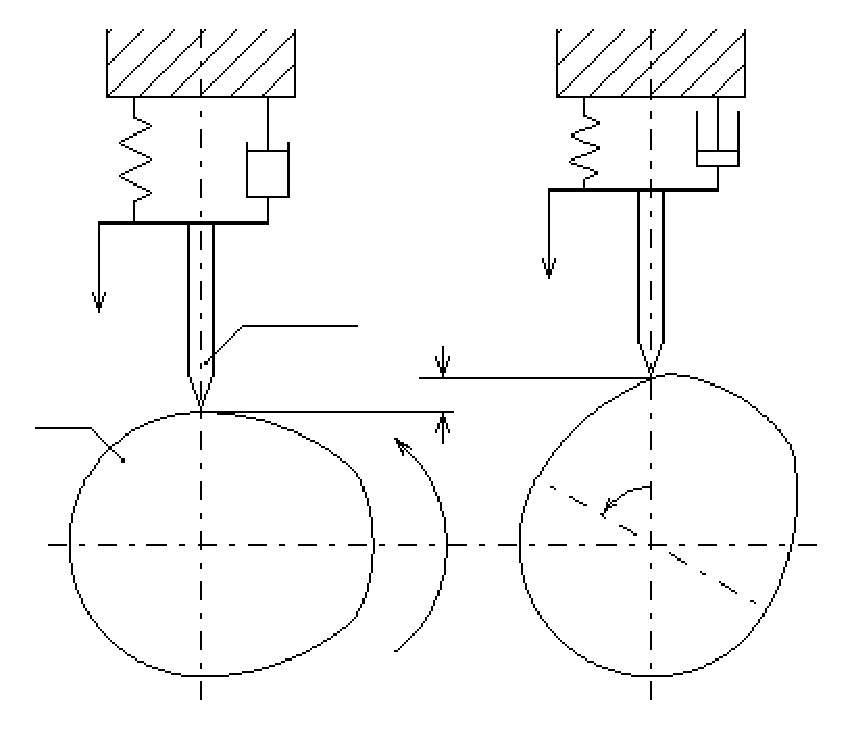
\includegraphics[height=8cm]{./Figures/cam}}}
 \put (0,52){\mbox{$F_{v}$}}
 \put (2,34.5){\mbox{\textit{Cam}}}
 \put (26,46){\mbox{\textit{Follower}}}
 \put (15,46){\mbox{\textit{$\mu$}}}
 \put (9,62){\mbox{$\kappa$}}
 \put (32,62){\mbox{$\zeta$}}
 \put (38,40){\mbox{$\delta c (\beta)$}}
 \put (66,28){\mbox{$\beta$}}
 \put (2.5,6){\mbox{\textit{$t=0$}}}
 \put (52.4,6){\mbox{\textit{$t=\beta$}}}
 \put (18.5,-1){\mbox{\textit{(a)}}}
 \put (69.4,-1){\mbox{\textit{(b)}}}
\end{picture}
\begin{picture}(90,80)(-3,0)
 \put (0,0){\mbox{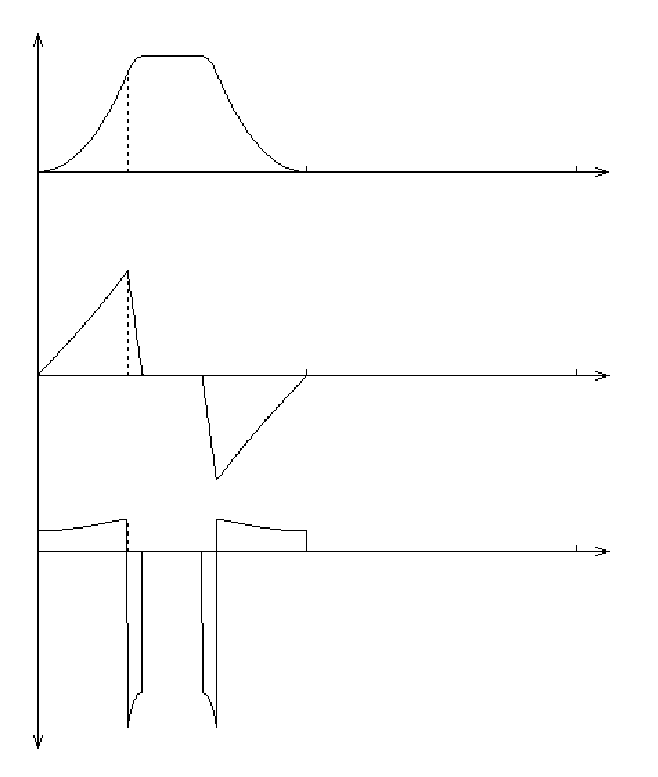
\includegraphics[height=8cm]{./Figures/campva}}}
 \put (-3,75){\mbox{$\delta c$}}
 \put (-3,49){\mbox{$ \frac{dc}{dt}$}}
 \put (-3,25){\mbox{$ \frac{d^2c}{dt^2}$}}
 \put (30,60){\mbox{$\pi$}} \put (58,60){\mbox{$2\pi$}}
 \put (10,60){\mbox{$\beta$}}
% \put (30,38){\mbox{$\pi$}} \put (58,38){\mbox{$2\pi$}}
% \put (9,38){\mbox{$\beta$}}
% \put (30,19){\mbox{$\pi$}} \put (58,19){\mbox{$2\pi$}}
% \put (9,19){\mbox{$\beta$}}
 \put (32,-1){\mbox{\textit{(c)}}}
\end{picture}
%\begin{picture}(45,20)(-90,-20)
% \put (3,10){\mbox{$v^{+}=(1+r)\frac{dc}{dt}-rv^{-}$}}
% \put (16,-1){\mbox{\textit{(d)}}}
%\end{picture}
%\begin{picture}(45,20)(-85,-20)
% \put (-2,20){\mbox{$k \hspace{4mm}= \hspace{1.5mm}5 \times 10^{4}\hspace{1.5mm} (N /m)$}}
% \put (-2,16){\mbox{$b \hspace{4mm}= \hspace{1.5mm}0 \hspace{10.5mm}(N\hspace{0.5mm} s/m)$}}
% \put (-2,12){\mbox{$F_{ext} \hspace{0.2mm}= \hspace{1.5mm}0 \hspace{12.5mm}(N)$}}
% \put (-2,8){\mbox{$c \hspace{4mm}\in \hspace{1.5mm}[0.52\hspace{2mm} 0.67]\hspace{2mm}(m)$}}
% \put (-2,4){\mbox{$r \hspace{4mm}= \hspace{1.5mm}0.9$}}
% \put (16,-1){\mbox{\textit{(e)}}}
%\end{picture}
  \caption{Cam-Shaft's schematics. \textit{(a)} t=0. \textit{(b)} t=$\beta$. \textit{(c)} Constraint position $\delta c(t)$, velocity $\frac{dc}{dt}(t)$ and acceleration $\frac{d^{2}c}{dt}(t^{2})$.}
  \label{Fig:cam-shaft}
\end{figure}
\subsection{The cam-follower as a Lagrangian NSDS.}
%\textit{\textbf{WP2 Template 1 Simulation of a bouncing ball with the Moreau's Time-Stepping scheme.}\\{Acary}}\\
 It is possible to completely describe the cam-follower system as a
 driven impact oscillator into the framework of \textit{Lagrangian NSDS} using a
translation in space. Setting $\hat u(t)=u(t)-c(t)$ and $\hat
v(t)= v(t)-dc/dt$, then equations (\ref{eq:sols}) and
(\ref{eq:il}) can be expressed as (the argument $t$ will not be
explicitly written)
\begin{eqnarray}
  \label{eq:trans}
  \mu\frac{d^2\hat u}{dt^2}+\zeta\frac{d\hat u}{dt}+\kappa
  \hat u=f_{v}-\left(\mu\frac{d^2c}{dt^2}+\zeta\frac{dc}{dt}+\kappa
  c\right)&\equiv &\hat f,  \; \text{\hspace{6.5mm} \text{if} \hspace{3mm}$\hat u >
 0$.}\\
\hat v^+&=&-r \hat v^- , \; \text{ \text{if}\hspace{3mm}$\hat
u=0$.}
\end{eqnarray}
Using the framework presented in [2] we have that the equation of
motion of a Lagrangian system may be stated as follows :
\begin{eqnarray}
  \label{eq:lag1}
  M(q)\ddot q + Q(q,\dot q) + F(\dot q, q , t) = F_{ext}(t) + R
\end{eqnarray}

From the (\ref{eq:trans}) we can derive all of the terms which
define a Lagrangian NSDS. In our case the model is completely
linear:
\begin{eqnarray}
  \nonumber
  q&=& \left[\begin{array}{c}  \hat u  \end{array}\right]    \\
  \nonumber
  M(q)&=&  \left[\begin{array}{c} \mu  \end{array}\right] \\
  \label{eq:lag2}
  Q(q,\dot q )& = &\left[\begin{array}{c} 0  \end{array}\right]  \\
  \nonumber
  F(q, \dot q ) &=&  \left[\begin{array}{c} \zeta \end{array}\right] \dot q +  \left[\begin{array}{c} \kappa  \end{array}\right] q\\
  \nonumber
  F_{ext}& = & \left[\begin{array}{c} \hat f \end{array}\right]
\end{eqnarray}

The unilateral constraint requires that:
\begin{eqnarray}
\label{eq:constr} \nonumber
 \hat u \geq 0
\end{eqnarray}
so we can obtain
\begin{eqnarray}
y &= & H^T q + b \\
\nonumber H^T &=&\left[\begin{array}{c} 1 \end{array}\right]\\
\nonumber b&=&0
\end{eqnarray}

In the same way, the reaction force due to the constraint is
written as follows:
\begin{eqnarray}
\nonumber R=H \lambda, \hspace{1cm}  \text{with }
H=\left[\begin{array}{c} 1
\end{array}\right]
\end{eqnarray}

The unilataral contact law may be formulated as follow:
\begin{eqnarray}
  \label{eq:17}
  0 \leq y \perp \lambda\geq 0
\end{eqnarray}
and the Newton's impact law:
\begin{eqnarray}
  \label{eq:17}
\text{If } y=0, \dot{y}^+ =-r\dot{y}^-
\end{eqnarray}

\subsection{Implementation in the platform}
%The code for the simulation of the Cam Follower system using the
%SICONOS software package is:
For the simulation of the cam follower system follow the steps

\begin{enumerate}
\item Move to the working directory \verb"sample/CamFollower"

\verb"$cd sample/CamFollower "

\item Clean the directory form binary files using the
\verb"siconos" command

\verb"$siconos -c "

\item Compile the file \verb"CamFollowerNoXml.cpp" in
the sample folder ({\em See} the code at the end of the section)

\verb"$siconos CamFollowerNoXml.cpp"

\item Change the simulation parameters ({\em i.e.}
Follower initial position and velocity, cam initial angle,
simulations time, cam rotational speed in rpm, etc.) in the file
\verb"CamFollowerNoXml.cpp".

\end{enumerate}

Next we present the sample code for the
\verb"CamFollowerNoXml.cpp" file:
\begin{tabbing}
\hspace{1cm}\= \hspace{0.5cm}\= \hspace{1cm}\= \hspace{1cm}\= \hspace{1cm}\\
 \> \+ int main(int argc, char* argv[]) {\bf \{} \\
 \>  {\bf\{} \+ \hspace{0.5cm}\= \hspace{2cm}\= \hspace{1cm}\=\hspace{1cm}\=\hspace{1cm}\=\hspace{1cm}\=\\
 \> \em   // ======== Creation of the model =============\\
 \> \em  // User-defined main parameters\\

 \> double rpm=358; \\
 \> double phi\_0=0;\\

 \> unsigned int dsNumber = 1; \>\>\>\> \em // the Follower and the ground\\
 \> unsigned int nDof = 1;  \>\>\>\>    \em // degrees of freedom for the Follower\\
 \> double t0 = 0;            \>\>\>\>  \em   // initial computation time\\
 \> double T = 5;             \>\>\>\>  \em    // final computation time\\
 \> double h = 0.0001;   \>\>\>\>       \em // time step\\
 \> int Kplot;\\
 \> Kplot=(int)(Tplot/h);\\

 \> double position\_init = 0.4;\>\>\>\> \em// initial position for lowest bead.\\
 \> double velocity\_init = 0.4;\>\>\>\> \em// initial velocity for lowest bead.\\
 \\
 \> \em    // ======= Dynamical systems =========\\
 \\
 \>     vector<DynamicalSystem *> vectorDS; // the list of DS\\
 \>     vectorDS.resize(dsNumber,NULL);\\
\\
 \> SiconosMatrix *Mass, *K, *C;        // mass/rigidity/viscosity\\
 \> Mass = new SiconosMatrix(nDof,nDof);\\
 \> (*Mass)(0,0) = 1.221;\\
 \> K = new SiconosMatrix(nDof,nDof);\\
 \> (*K)(0,0) = 1430.8;\\
 \> C = new SiconosMatrix(nDof,nDof);\\
 \> (*C)(0,0) = 0;\\
\\
 \>  //  Initial positions and velocities  \\
 \>  vector<SimpleVector *> position\_0;\\
 \>  vector<SimpleVector *> velocity\_0;\\
 \>  position\_0.resize(dsNumber,NULL);\\
 \>  velocity\_0.resize(dsNumber,NULL);\\
 \>  position\_0[0] = new SimpleVector(nDof);\\
 \>  velocity\_0[0] = new SimpleVector(nDof);\\
 \>  (*(position\_0[0]))(0) = position\_init;\\
 \>  (*(velocity\_0[0]))(0) = velocity\_init;\\
 \\
 \>  vectorDS[0] =\\ \>
 new LagrangianLinearTIDS(0,nDof,*(position\_0[0]),*(velocity\_0[0]),*Mass,*K,*C);\\
\\
 \> static\_cast<LagrangianDS*>(vectorDS[0])
 \\ \>\>\>->setComputeFExtFunction("FollowerPlugin.so", "FollowerFExt");\\
\\
 \> // Example to set a list of parameters in FExt function.\\
 \> // 1 - Create a simple vector that contains the required
 parameters.\\
\\
 \> // Here we set two parameters, the DS  number.\\
 \> SimpleVector * param = new SimpleVector(2);\\
\\
 \> (*param)(0)=rpm;\\
 \> (*param)(1)=phi\_0;\\
 \> // 2 - Assign this param to the function FExt\\
 \> static\_cast<LagrangianDS*>(vectorDS[0])->setParametersListPtr(param,2);\\
 \> // 2 corresponds to the position of FExt in the stl vector of possible parameters. \\
\> //  0 is mass, 1 FInt.\\ % and so on.\\
 \> // Now the cam rotational velocity in rpms will be available in FExt plugin.\\
\\
\> // ===== Interactions =====\\
\\
 \>  vector<Interaction*> interactionVector;\\
 \>  interactionVector.resize(1,NULL);\\
 \>  vector<DynamicalSystem*> *dsConcerned = \\ \>\>\> new vector<DynamicalSystem*>(dsNumber);\\
\\
 \>  // ===== Non Smooth Law =====\\
 \>  double e = 0.8;\\

 \>  // Interaction Follower-floor\\
 \>  SiconosMatrix *H = new SiconosMatrix(1,nDof);\\
 \>  (*H)(0,0) = 1.0;\\
 \>  NonSmoothLaw * nslaw = new NewtonImpactLawNSL(e);\\
 \>  Relation * relation = new LagrangianLinearR(*H);\\
 \>  (*dsConcerned)[0] = vectorDS[0];\\

 \>  interactionVector[0] = new Interaction("Follower-Ground",0,1, dsConcerned);\\
 \>  interactionVector[0]->setRelationPtr(relation);\\
 \>  interactionVector[0]->setNonSmoothLawPtr(nslaw);\\

 \> // ===== Interactions =====\\
\\
 \> // ===== NonSmoothDynamicalSystem =====\\

 \> bool isBVP =0;\\
 \> NonSmoothDynamicalSystem * nsds = \\
\>\>\>\> new NonSmoothDynamicalSystem(isBVP);\\
\\
 \>// Set DS of this NonSmoothDynamicalSystem\\
 \> nsds->setDynamicalSystems(vectorDS);       \\
 \> // Set interactions of the  NonSmoothDynamicalSystem\\
 \> nsds->setInteractions(interactionVector);  \\
\\
 \> // ===== Model =====\\
\\
 \> Model * Follower = new Model(t0,T);\\
 \> // set NonSmoothDynamicalSystem of this  model\\
 \> Follower->setNonSmoothDynamicalSystemPtr(nsds);\\
 \\
 \> // ====== Strategy ======\\
\\
 \> double theta = 0.5;  \>\>\>      // theta for Moreau integrator\\
 \> string solverName = "QP" ;\\
\\
 \> Strategy* S = new TimeStepping(Follower);\\
\\
 \> // -- Time discretisation --\\
 \> TimeDiscretisation * t = new TimeDiscretisation(h,S);\\
\\
 \> // -- OneStepIntegrators --\\
 \> vector<OneStepIntegrator *> vOSI;\\
 \> vOSI.resize(dsNumber,NULL);\\
 \> vOSI[0] = new Moreau(t,vectorDS[0],theta);\\
 \> S->setOneStepIntegrators(vOSI);\\
\\
 \> // -- OneStepNsProblem --\\
 \> OneStepNSProblem * osnspb = new LCP(S,solverName,101, 0.0001,"max",0.6);\\
 \> S->setOneStepNSProblemPtr(osnspb); // set OneStepNSProblem of the
 strategy\\
 \> cout << "=== End of model loading === " << endl;\\
 \> // ==== End of model definition======\\
\\
\\
\\
 \> // ========= Computation============\\
\\
 \> // --- Strategy initialization ---\\
 \> S->initialize();\\
 \> cout <<"End of strategy initialisation" << endl;\\
\\

 \> int k = t->getK(); \> \> \> \> // Current step\\
 \> int N = t->getNSteps(); \> \> \> \> // Number of time steps\\
\\
 \> // --- Get the values to be plotted ---\\
 \> // -> saved in a matrix dataPlot\\
 \> unsigned int outputSize = 8;\\
\\
 \> SiconosMatrix DataPlot(Kplot+1,outputSize );\\
 \>   // For the initial time step:\\
 \\
 \> // time\\
 \>     DataPlot(k,0) = k*t->getH();\\
 \\
 \>     DataPlot(k,1) = static\_cast<LagrangianDS*>(vectorDS[0])->getQ()(0);\\
 \>     DataPlot(k,2) = static\_cast<LagrangianDS*>(vectorDS[0])->getVelocity()(0);\\
 \>     DataPlot(k,3) = (Follower->getNonSmoothDynamicalSystemPtr()->\\
 \> \> getInteractionPtr(0)->getLambda(1))(0);\\
 \>     DataPlot(k,4) = static\_cast<LagrangianDS*>(vectorDS[0])->getFExt()(0);\\
 \\
 \>     // State of the Cam\\
 \>      double CamEqForce,CamPosition,CamVelocity,CamAcceleration;\\

 \>     CamEqForce=\\
 \> \> CamState(k*t->getH(),rpm,CamPosition,CamVelocity,CamAcceleration);\\
 \>     // Position of the Cam\\
 \>      DataPlot(k, 5) = CamPosition;\\
 \>      // Velocity of the Cam\\
 \>      DataPlot(k, 6) = CamVelocity;\\
 \>      // Acceleration of the Cam\\
 \>      DataPlot(k, 7) =\\
 \> \>CamPosition+static\_cast<LagrangianDS*>(vectorDS[0])->getQ()(0);\\
\\
 \> // --- Time loop ---\\
 \> cout << "Start computation ... " << endl;\\
 \> while(k < N)\\
 \>   {\bf \{ }\+ \hspace{0.5cm}\= \hspace{2cm}\= \hspace{1cm}\=\hspace{1cm}\=\hspace{1cm}\=\hspace{1cm}\=\\\\
 \> // --- Get values to be plotted ---\\
 \>     DataPlot(k,0) = k*t->getH();\\
 \\
 \>     DataPlot(k,1) = \\
 \> \> static\_cast<LagrangianDS*>(vectorDS[0])->getQ()(0);\\
 \>     DataPlot(k,2) =  \\
 \> \> static\_cast<LagrangianDS*>(vectorDS[0])->getVelocity()(0);\\
 \>     DataPlot(k,3) =  \\
 \> \> (Follower->getNonSmoothDynamicalSystemPtr()->\\
 \> \> getInteractionPtr(0)->getLambda(1))(0);\\
 \>     DataPlot(k,4) = static\_cast<LagrangianDS*>(vectorDS[0])->getFExt()(0);\\
 \\

 \>     CamEqForce=\\
 \>  CamState(k*t->getH(),rpm,CamPosition,CamVelocity,CamAcceleration);\\
 \\
 \>      DataPlot(k, 5) = CamPosition;\\
 \>      DataPlot(k, 6) = CamVelocity;\\
 \>      DataPlot(k, 7) = CamPosition+\\
 \> \> static\_cast<LagrangianDS*>(vectorDS[0])->getQ()(0);\\

 \> // transfer of state i+1 into state i and time
 incrementation\\
 \> S->nextStep();\\

 \> // get current time step\\
 \> k = t->getK();\\
 \> // solve ...\\
 \> S->computeFreeState();\\
 \> S->computeOneStepNSProblem();\\
 \> // update\\
 \> S->update();
 \-\\
 \>   {\bf \} }\\
\>    // --- Output files ---\\
 \> DataPlot.rawWrite("result.dat", "ascii");\\

 \> // --- Free memory ---\\
 \> delete osnspb;\\
 \> delete vOSI[0];\\
 \> delete t;\\
 \> delete S;\\
 \> delete Follower;\\
 \> delete nsds;\\
 \> delete interactionVector[0];\\
 \> delete relation;\\
 \> delete nslaw;\\
 \> delete H;\\
 \> delete dsConcerned;\\
 \> delete vectorDS[0];\\
 \> delete position\_0[0];\\
 \> delete velocity\_0[0];\\
 \> delete C;\\
 \> delete K;\\
 \> delete Mass;\\

    \-\\
 \>  {\bf\}}
\end{tabbing}
%\end{enumerate}
\newpage
\subsection{Simulation}
We have perform the simulation of the cam follower system for
different values of the cam rotational speed with the SICONOS
software package using a time-stepping numerical scheme with step
size ($h=1e^{-4}$) and an event-driven scheme with minimum step
size \linebreak ($h_{min}=1e^{-12}$). Fig.
\ref{Fig:time_comparison} and \ref{Fig:state_comparison} show the
time simulations for different values of the cam rotational speed
and Fig. \ref{Fig:attractor_comparison} show the chaotic attractor
at $rpm=660$ for impact and stroboscopic Poincar\`e sections.

\begin{figure}[hbtp]
\vspace{5mm} \setlength{\unitlength}{1mm}
\begin{picture}(60,60)(0,-7)
 \put (0,0){\mbox{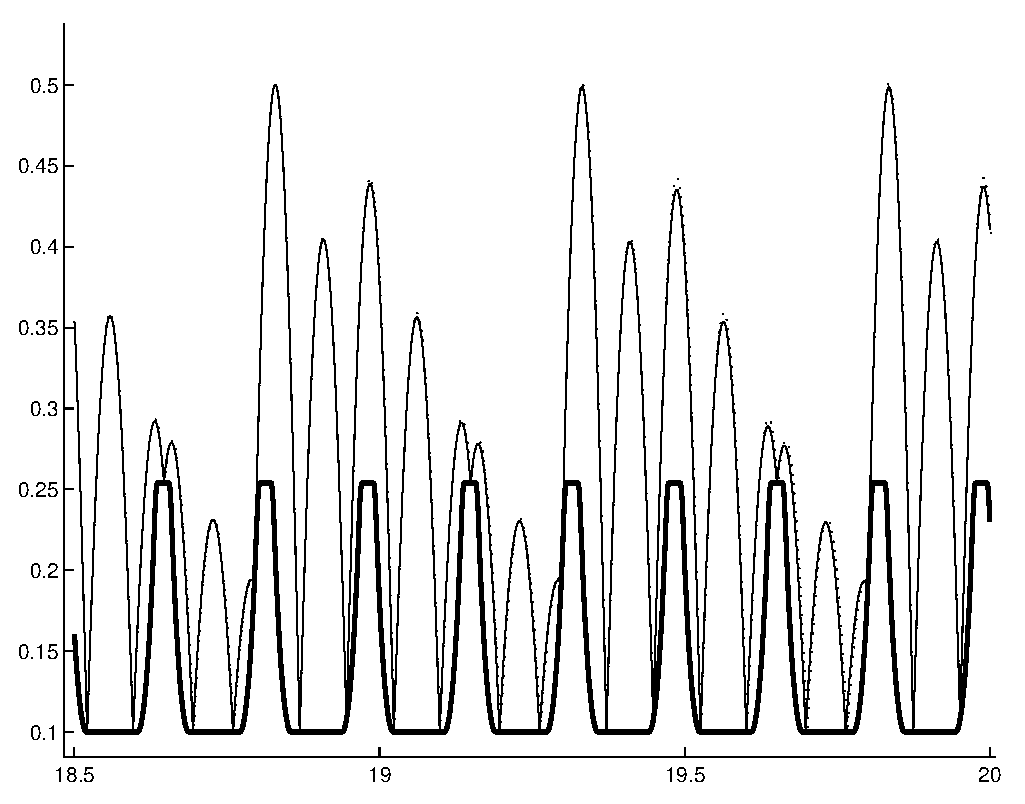
\includegraphics[height=6cm]{./comparison_figs/time_comparison_358}}}
  \put (35,-4){\mbox{\textit{(a)}}}
\end{picture}
\begin{picture}(60,60)(15,-7)
 \put (0,0){\mbox{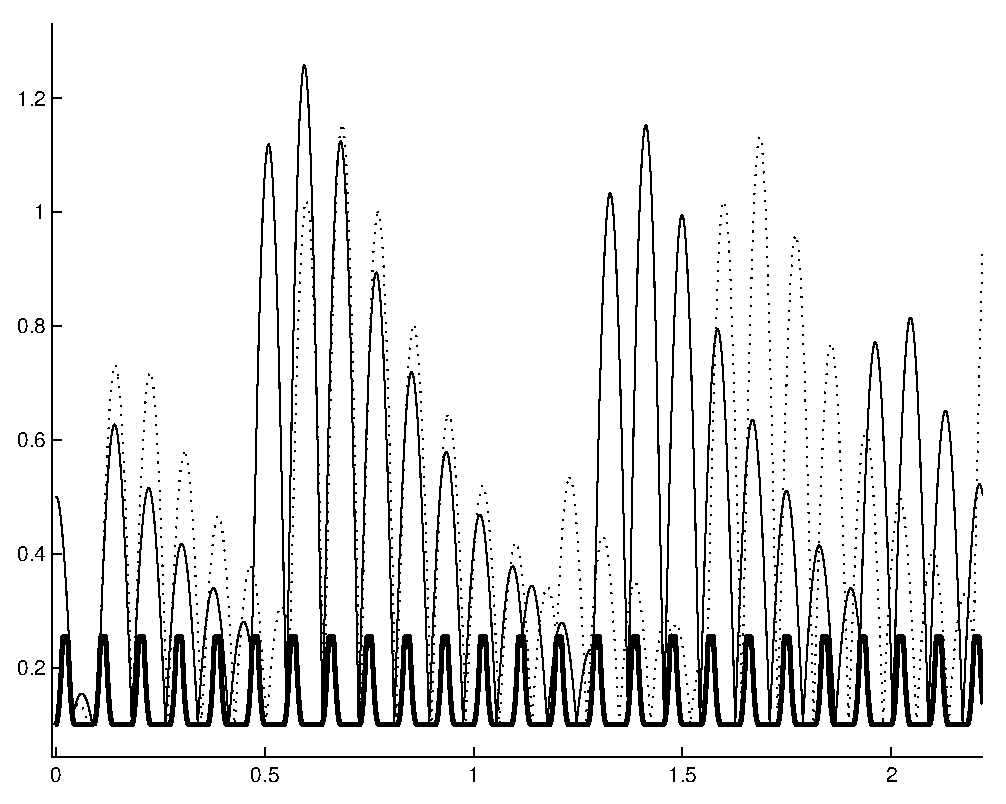
\includegraphics[height=6cm]{./comparison_figs/time_comparison_660}}}
 \put (35,-4){\mbox{\textit{(b)}}}
\end{picture}
\begin{picture}(60,60)(-40,-2)
 \put (0,0){\mbox{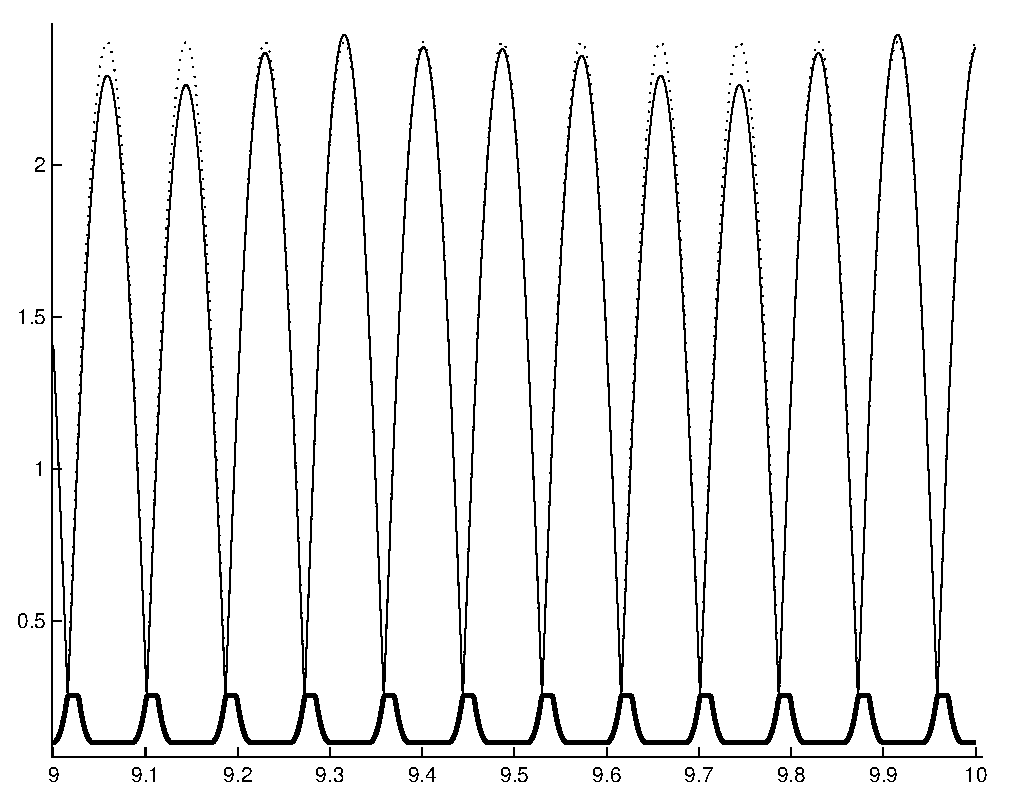
\includegraphics[height=6cm]{./comparison_figs/time_comparison_700}}}
 \put (35,-4){\mbox{\textit{(c)}}}
\end{picture}
  \caption{Time series using SICONOS platform. Time-stepping scheme (continuous line). Event-driven scheme (dashed line) \textit{(a)} rpm=358. \textit{(b)} rpm=660. \textit{(c)} rpm=700.}
  \label{Fig:time_comparison}
\end{figure}

\begin{figure}[hbtp]
\vspace{5mm} \setlength{\unitlength}{1mm}
\begin{picture}(60,60)(0,-7)
 \put (0,0){\mbox{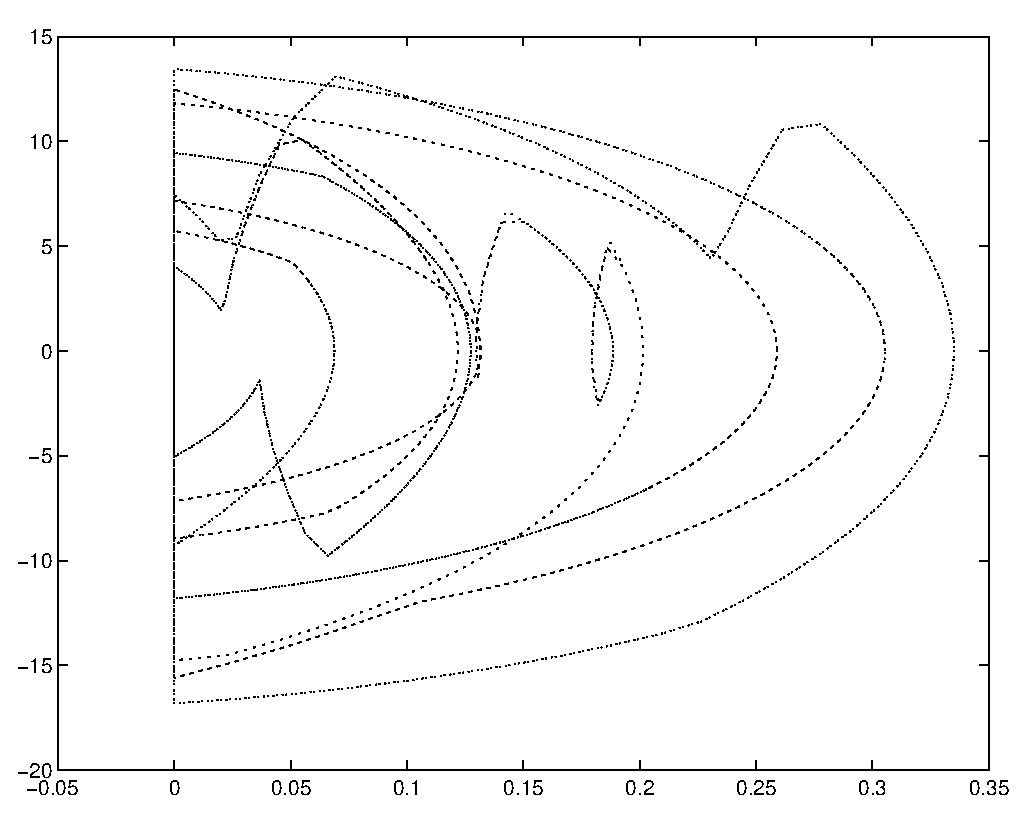
\includegraphics[height=6cm]{./comparison_figs/state_comparison_358event}}}
  \put (35,-4){\mbox{\textit{(a)}}}
\end{picture}
\begin{picture}(60,60)(15,-7)
 \put (0,0){\mbox{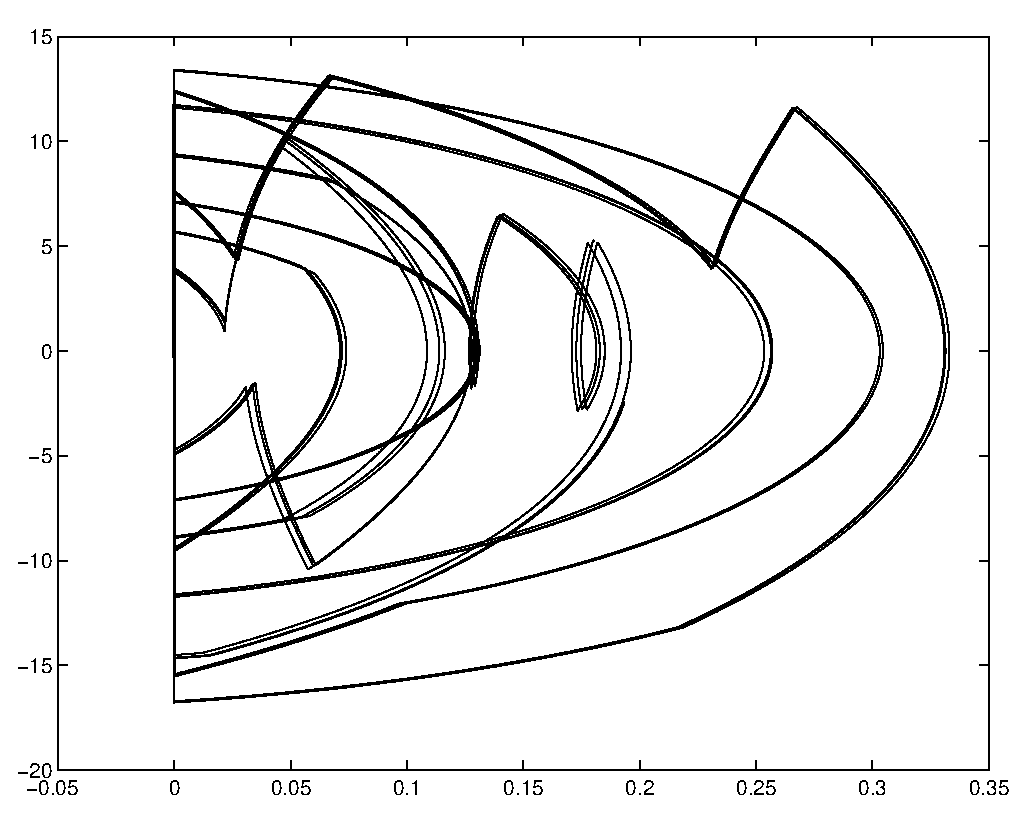
\includegraphics[height=6cm]{./comparison_figs/state_comparison_358siconos}}}
 \put (35,-4){\mbox{\textit{(b)}}}
\end{picture}
\begin{picture}(60,60)(0,-2)
 \put (0,0){\mbox{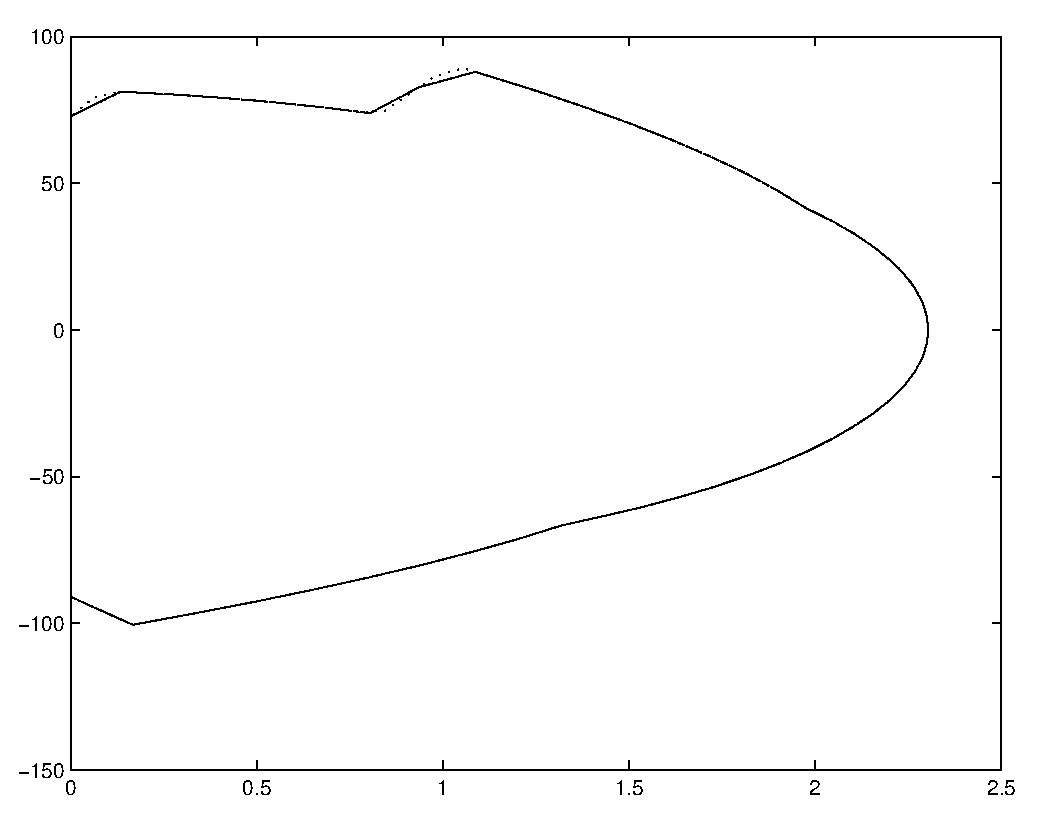
\includegraphics[height=6cm]{./comparison_figs/state_comparison_700event}}}
  \put (35,-4){\mbox{\textit{(c)}}}
\end{picture}
\begin{picture}(60,60)(-17,-2)
 \put (0,0){\mbox{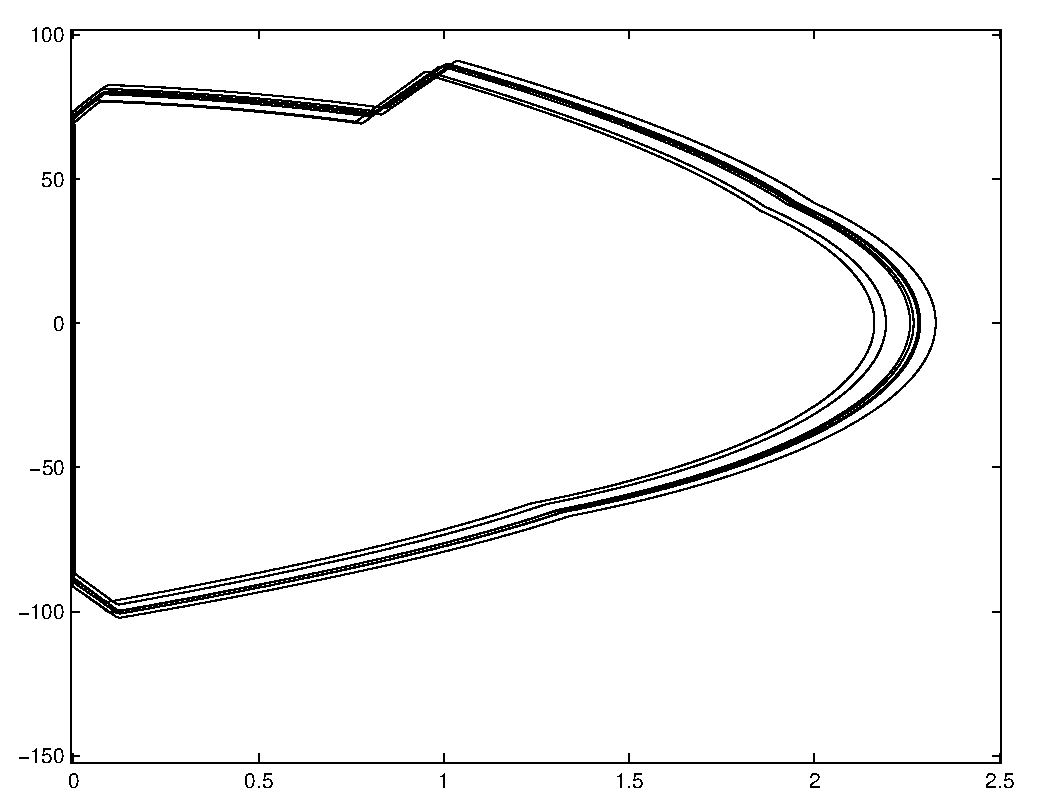
\includegraphics[height=6cm]{./comparison_figs/state_comparison_700siconos}}}
 \put (35,-4){\mbox{\textit{(d)}}}
\end{picture}
  \caption{State space comparison using SICONOS platform. \textit{(a)} rpm=358. Event Driven \textit{(b)} rpm=358. Time Stepping ($h=1e^{-4}$)\textit{(c)} rpm=700. Event Driven \textit{(d)} rpm=700. Time Stepping ($h=1e^{-4}$)}
  \label{Fig:state_comparison}
\end{figure}

\begin{figure}[hbtp]
\vspace{5mm} \setlength{\unitlength}{1mm}
\begin{picture}(60,60)(0,-7)
 \put (0,0){\mbox{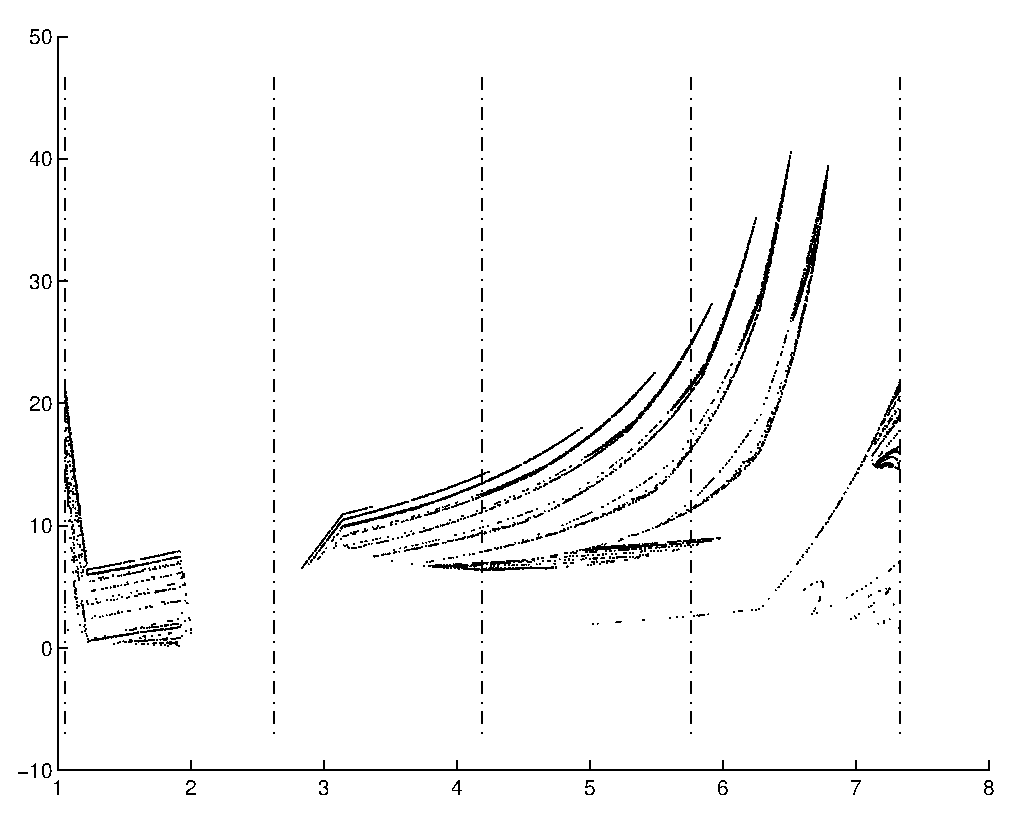
\includegraphics[height=6cm]{./comparison_figs/impact_map_660event}}}
  \put (35,-4){\mbox{\textit{(a)}}}
\end{picture}
\begin{picture}(60,60)(15,-7)
 \put (0,0){\mbox{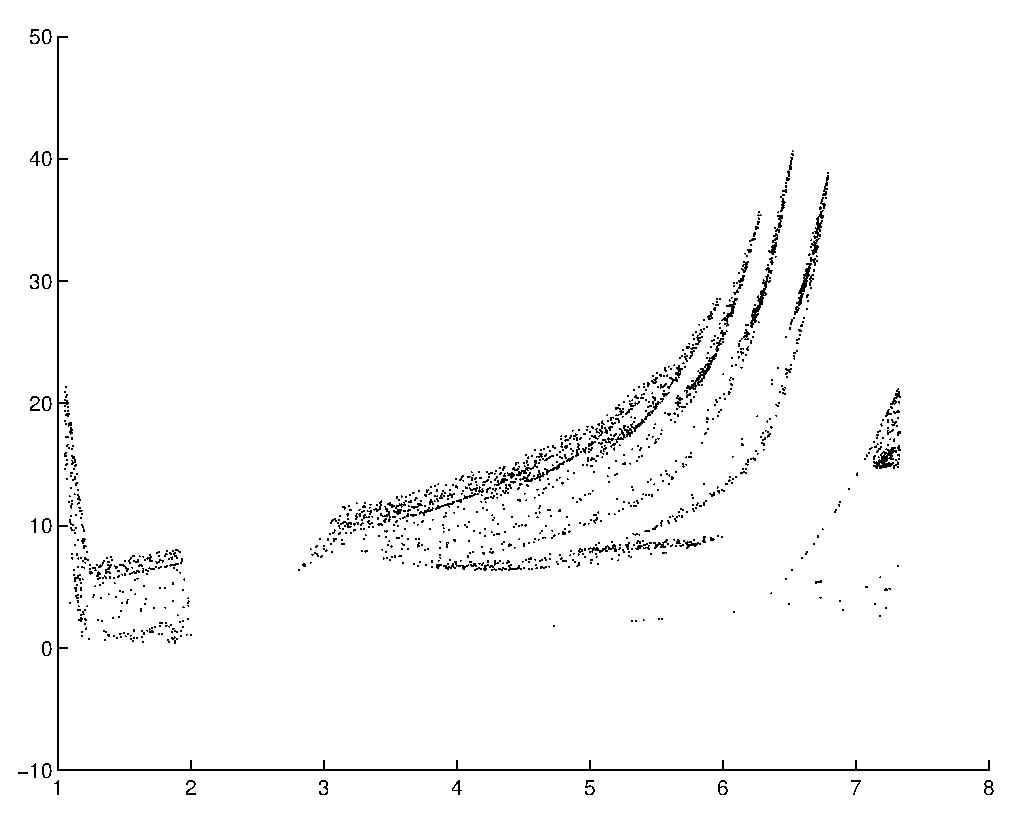
\includegraphics[height=6cm]{./comparison_figs/impact_map_660siconos}}}
 \put (35,-4){\mbox{\textit{(b)}}}
\end{picture}
\begin{picture}(60,60)(0,-2)
 \put (0,0){\mbox{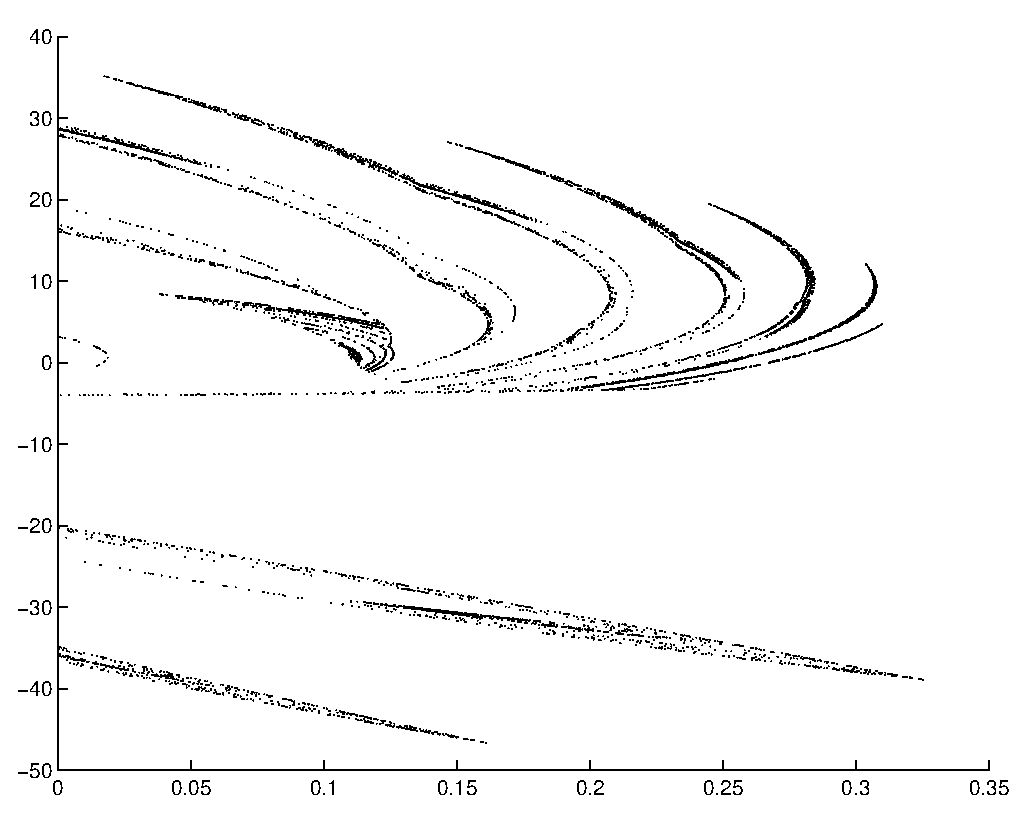
\includegraphics[height=6cm]{./comparison_figs/stroboscopic_map_660event}}}
  \put (35,-4){\mbox{\textit{(c)}}}
\end{picture}
\begin{picture}(60,60)(-17,-2)
 \put (0,0){\mbox{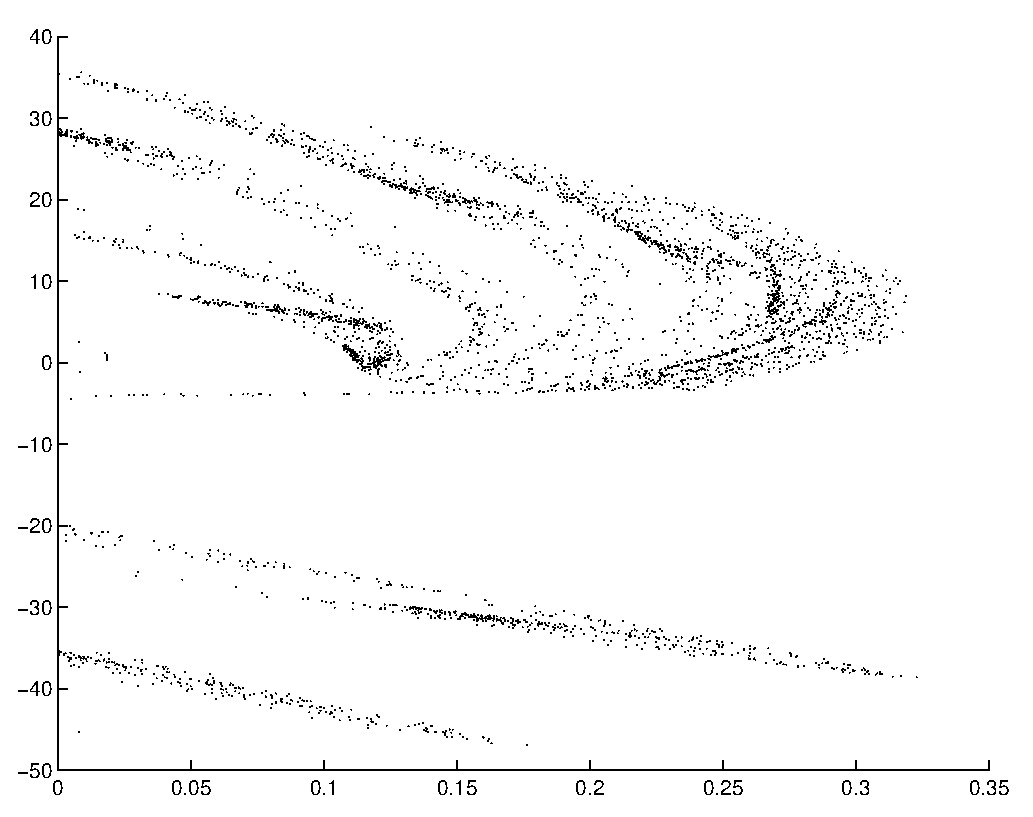
\includegraphics[height=6cm]{./comparison_figs/stroboscopic_map_660siconos}}}
 \put (35,-4){\mbox{\textit{(d)}}}
\end{picture}
  \caption{Attractors comparison using SICONOS platform at rpm=660. \textit{(a)}  Impact map. (Event Driven) \textit{(b)} Impact Map. Time Stepping ($h=1e^{-4}$)\textit{(a)}  Stroboscopic map. (Event Driven) \textit{(b)} Stroboscopic Map. Time Stepping ($h=1e^{-4}$)}
  \label{Fig:attractor_comparison}
\end{figure}

\chapter{Quartic Formulation}


\subsection{Slidding ?}
It consists in finding $\alpha >0$ and $R \in \partial K_{\mu}$ such that $-\alpha \left(\begin{array}{l} 0\\ R_T\end{array}\right)=MR+q$. That is :
  \begin{equation}
\label{eq_quartic1}
\left[\begin{array}{c}
M+ \left(\begin{array}{ccc} 0&0&0\\ 0&\alpha&0 \\ 0&0&\alpha \end{array}\right)
\end{array}\right]R+q=0
\end{equation}

  \subsubsection{$R_T$ is on a conic}
  The first line of the system~\ref{eq_quartic1} and the $R \in \partial K_{\mu}$ is the intersection between a plan and a cone in $\mathbb{R}^3$, endeed:
  \begin{equation}
\label{eq_quartic2}
\begin{array}{l}
 \mu R_N =  \parallel R_T \parallel  \\
\frac{M_{11}}{\mu} \parallel R_T \parallel = -q_1-M_{12}R_{T1}-M_{13}R_{T2}
\end{array}
\end{equation}
That is:
\begin{equation}
\label{eq_quartic2}
\begin{array}{l}
\mu^2 R_N^2 =  (R_{T1}^2 +R_{T1}^2)  \\
\frac{M_{11}^2}{\mu^2} (R_{T1}^2 +R_{T1}^2)=(-q_1-M_{12}R_{T1}-M_{13}R_{T2})^2
\end{array}
\end{equation}
That means that $R_T$ is contained in a conic,  focus and directrice are:
\begin{equation}
\label{eq_quartic3}
\begin{array}{l}
\mathcal{D} : q_1+M_{12}R_{T1}+M_{13}R_{T2} =0  \\
focus : \mathcal{O}\\
\frac{M_{11}^2}{\mu^2}  Dist(\mathcal{O}, R_T) ^2=Dist(\mathcal{D},R_T)^2 (M_{12}^2+M_{13}^2)\\
\frac{Dist(\mathcal{O}, R_T)}{Dist(\mathcal{D},R_T)}=\frac{\mu\sqrt{(M_{12}^2+M_{13}^2)}}{M_{11} }=e
\end{array}
\end{equation}
The parametric equation is:
\begin{equation}
\label{eq_quartic4}
\begin{array}{l}
R_{T1}=r cos(\theta )\\
R_{T2}=r sin(\theta )\\
r=\frac{p}{1+ecos(\theta - \phi)}
\end{array}
\end{equation}
With $p$ an simple expression of $M_{11},M_{12},M_{13}$, and $\phi$ a constant angle between $\mathcal{D}$ and $(O,R_{T1})$
\subsubsection{The two last line of the system~\ref{eq_quartic1}}
\begin{equation}
\label{eq_quartic5}
\frac{\parallel R_T \parallel}{\mu} \tilde M_{1.} +\left(\tilde M+\left(\begin{array}{cc} \alpha&0 \\ 0&\alpha \end{array}\right)\right)R_T+\tilde q=0
\end{equation}
$\tilde M$ is symetric, so it exists a unitary matrix $V$ such that $V \tilde M V^T = \left(\begin{array}{cc} d_1&0 \\ 0&d_2 \end{array}\right)$.  One can get:
\begin{equation}
\label{eq_quartic6}
\frac{\parallel R_T \parallel}{\mu} V \tilde M_{1.} +V \left(\tilde M+\left(\begin{array}{cc} \alpha&0 \\ 0&\alpha \end{array}\right)\right)V^TVR_T+V\tilde q=0
\end{equation}
Rename:
\begin{equation}
\label{eq_quartic7}
  \frac{\parallel \bar R_T \parallel}{\mu} \bar M_{1.} +\left(\begin{array}{cc} d_1+\alpha&0 \\ 0&d_2+\alpha \end{array}\right)\overline R_T+\bar q=0
  \end{equation}
In the plan, either $V$ is a rotation or a symetrie. So $ \bar R_T=VR_T$ is a conic with the same focus and a rotated directrice, it means that it exists $\phi_1$ such that :

\begin{equation}
\label{eq_quartic8}
\begin{array}{l}
\bar R_{T1}=r cos(\theta )\\
\bar R_{T2}=r sin(\theta )\\
r=\frac{p}{1+ecos(\theta - \phi_1)}
\end{array}
\end{equation}
The equation~\ref{eq_quartic7} is :
\begin{equation}
\label{eq_quartic9}
\begin{array}{l}
  (d_1+\alpha)\bar R_{T1}=-\bar q_1+a_1 \parallel R_T \parallel\\
(d_2+\alpha)\bar R_{T2}=-\bar q_2+a_2 \parallel R_T \parallel
\end{array}
\end{equation}
The case ($\bar R_{T1} = 0$ or  $\bar R_{T2} = 0$) has to be examine. We try to eliminate $alpha$:
\begin{equation}
\label{eq_quartic10}
  \begin{array}{l}
    d_1 \bar R_{T1} \bar R_{T2}+\alpha \bar R_{T1} \bar R_{T2} =-\bar q_1\bar R_{T2}+a_1 \bar R_{T2} \parallel R_T \parallel\\
d_2 \bar R_{T1} \bar R_{T2}+\alpha \bar R_{T1} \bar R_{T2} =-\bar q_2\bar R_{T1}+a_2 \bar R_{T1} \parallel R_T \parallel
\end{array}
\end{equation}
that leads to:
\begin{equation}
\label{eq_quartic10}
  (d_1-d_2) \bar R_{T1} \bar R_{T2}=-\bar q_1\bar R_{T2}+\bar q_2\bar R_{T1}+(a_1 \bar R_{T2}-a_2 \bar R_{T1}) \parallel R_T \parallel\\
\end{equation}
The parametric expression of $\bar R_T$ leads to:
\begin{equation}
\label{eq_quartic11}
\begin{array}{l}
  (d_1-d_2)r^2cos(\theta )sin(\theta )=-\bar q_1rsin(\theta )+\bar q_2rcos(\theta )+r(a_1 rsin(\theta )-a_2 rcos(\theta )) \\
  \textrm{ie:}(d_1-d_2)rcos(\theta )sin(\theta )=-\bar q_1sin(\theta )+\bar q_2cos(\theta )+r(a_1 sin(\theta )-a_2 cos(\theta ))\\
  \end{array}
\end{equation}
with the expression of r:
\begin{equation}
\label{eq_quartic12}
\begin{array}{l}
(d_1-d_2)\frac{p}{1+ecos(\theta - \phi_1)}cos(\theta )sin(\theta )=\\-\bar q_1sin(\theta )+\bar q_2cos(\theta )+\frac{p}{1+ecos(\theta - \phi_1)}(a_1  sin(\theta )-a_2 cos(\theta ))\\\\
\textrm{ie:}(d_1-d_2)pcos(\theta )sin(\theta )=\\(1+ecos(\theta - \phi_1))(-\bar q_1sin(\theta )+\bar q_2cos(\theta ))+p(a_1  sin(\theta )-a_2 cos(\theta ))\\\\
\textrm{ie:}(d_1-d_2)pcos(\theta )sin(\theta )=\\(1+e(cos(\theta)cos(\phi_1)+sin(\theta)sin(\phi_1)))(-\bar q_1sin(\theta )+\bar q_2cos(\theta ))+p(a_1  sin(\theta )-a_2 cos(\theta ))\\\\
\textrm{ie:}(d_1-d_2)pcos(\theta )sin(\theta )+\\(1+ecos(\theta)cos(\phi_1)+esin(\theta)sin(\phi_1))(\bar q_1sin(\theta )-\bar q_2cos(\theta ))+p(-a_1  sin(\theta )+a_2 cos(\theta ))=0
 \end{array}
\end{equation}
rename :
\begin{equation}
\label{eq_quartic13}
\begin{array}{l}
Acos(\theta )^2+Bsin(\theta)^2+Csin(\theta )cos(\theta )+Dsin(\theta )+Ecos(\theta )=0
 \end{array}
\end{equation}
with
\begin{equation}
\label{eq_quartic12}
\begin{array}{l}
A=- e\bar q_2cos(\phi_1)\\
B=e \bar q_1sin(\phi_1)\\
C=(d_1-d_2)p+ecos(\phi_1)\bar q_1-esin(\phi_1)\bar q_2\\
D=\bar q_1-pa_1\\
E=-\bar q_2+pa_2\\
\end{array}
\end{equation}
rename :
Using the following set of unknown :
\begin{equation}
\label{eq_quartic14}
\begin{array}{l}
t=tan(\theta /2)\\
sin(\theta )=\frac{2t}{1+t^2}\\
cos(\theta )=\frac{1-t^2}{1+t^2}
 \end{array}
\end{equation}
leads to:
\begin{equation}
\label{eq_quartic13}
\begin{array}{l}
  A\frac{(1-t^2)^2}{1+t^2} +B\frac{4t^2}{1+t^2}+ C\frac{2t(1-t^2)}{1+t^2}+D2t+E(1-t^2)=0\\
\textrm{ie:}A(1-t^2)^2 + 4Bt^2+C2t(1-t^2)+2Dt(1+t^2)+E(1-t^2)(1+t^2)=0\\\\
\textrm{ie:}P_4=A-E\qquad P_3=-2C+2D \qquad P_2=4B-2A \qquad P_1=2C+2D \qquad P_0=A+E
 \end{array}
\end{equation}
Finally, we get 4 possible values for $R_T$, checking the sign of $\alpha$ and $R_N$ selects the solutions.

\subsubsection{case $R_{T12}=0$}
From~\ref{eq_quartic9}, $R_{T1}$ leads to:
\begin{equation}
\label{eq_quartic14}
\begin{array}{l}
  \parallel R_T \parallel=|\bar R_{T2}|=\frac{\bar q_1}{a_1}\\\\
  \bar R_T=\left(\begin{array}{c} 0 \\ \pm \frac{\bar q_1}{a_1} \end{array}\right)
 \end{array}
\end{equation}

From~\ref{eq_quartic9}, $R_{T2}$ leads to:
\begin{equation}
\label{eq_quartic14}
\begin{array}{l}
  \parallel R_T \parallel=|\bar R_{T1}|=\frac{\bar q_2}{a_2}\\\\
  \bar R_T=\left(\begin{array}{c}  \pm \frac{\bar q_2}{a_2} \\ 0 \end{array}\right)
 \end{array}
\end{equation}

From $\bar R_T$, we have to check the coherence with the equation~\ref{eq_quartic8}. If it is on the conic,  we compute R, and the sign condition of the equation~\ref{eq_quartic1} must be check.



\chapter{Alart--Curnier Formulation}

\section{Reduced formulation to local variables.}

\subsection{Formulation}

Let us start with 
\begin{equation}
  \label{eq:AC-L7}
  \begin{array}{l}
  \varPhi_1(U,P) =  - U_{k+1}  + \widehat W P_{k+1}  + U_{\mathrm{free}}\\ \\
  \varPhi_2(U,P) =  P_{\n} - \proj_{\nbR^{a}_+} (P_{\n} - \rho_{\n}\circ (U_{\n} +e \circ  U_{\n,k}) ) \\ \\
  \varPhi_3(U,P) =  P_{\t} - \proj_{\widehat {\bf D}(P_{\n},U_{\n})} (P_{{\t}} - \rho_{\t}\circ \,U_{\t} )
\end{array}
\end{equation}
where the modified friction disk for a contact $\alpha$ is
\begin{equation}\label{eq:AC-L3}
  \widehat {\bf D}^\alpha(P^\alpha_{\n,k+1},U_{\n,k+1}^{\alpha}) = {\bf D}(\mu(\proj_{\nbR_+} (P^\alpha_{\n,k+1} - \rho^\alpha_{\n}\,(U_{\n,k+1}^{\alpha}+e^\alpha U_{\n,k}^{\alpha}) )).
\end{equation}
\subsection{Structure of the Jacobians}

Let us denote the one element of the  generalized Jacobian by  $ H(U,P) \in \partial \Phi(U,P)$ which has the structure
\begin{equation}
  \label{eq:AC-L6}
   H(U,P) = 
   \left[\begin{array}{cccc}
       - I & 0 &  \widehat W_{\n\n} & \widehat W_{\n\t} \\ \\
       0  & -I  &  \widehat W_{\t\n} & \widehat W_{\t\t} \\ \\
       \partial_{U_{\n}} \Phi_2(U,P) & 0 &   \partial_{P_{\n}} \Phi_2(U,P) & 0 \\ \\
       \partial_{U_{\n}} \Phi_3(U,P) &  \partial_{U_{\t}} \Phi_3(U,P) &  \partial_{P_{\n}} \Phi_3(U,P)  & \partial_{P_{\t}} \Phi_3(U,P)
   \end{array}\right]
\end{equation}


\subsection{Computation of the gradients}


Let us consider the single contact case.
\paragraph{Computation of the gradients of $\Phi_2$}
\begin{equation}
  \label{eq:AC-T1}
  \begin{array}{l}
  \varPhi_2(U,P) =  P_{\n} - \proj_{\nbR^{a}_+} (P_{\n} - \rho_{\n} (U_{\n} +e  U_{\n,k}) ) \\ \\
\end{array}
\end{equation}
\begin{itemize}
\item \textbf{If} $P_{\n} - \rho_{\n} (U_{\n} +e  U_{\n,k}) \geq 0 $, we get 
  \begin{equation}
    \label{eq:AC-T2}
    \begin{array}{l}
      \varPhi_2(U,P) =  + \rho_{\n} (U_{\n} +e  U_{\n,k})
    \end{array}
  \end{equation}
  and 
  \begin{equation}
    \label{eq:AC-T3}
    \begin{array}{l}
     \partial_{U_{\n}} \varPhi_2(U,P) =  + \rho_{\n} \\ \\
     \partial_{P_{\n}} \varPhi_2(U,P) =  0 \\ \\ 
    \end{array}
  \end{equation}
\item \textbf{If} $P_{\n} - \rho_{\n} (U_{\n} +e  U_{\n,k})  < 0 $, we get 
  \begin{equation}
    \label{eq:AC-T4}
    \begin{array}{l}
      \varPhi_2(U,P) =  P_{\n}
    \end{array}
  \end{equation}
  and 
  \begin{equation}
    \label{eq:AC-T5}
    \begin{array}{l}
     \partial_{U_{\n}} \varPhi_2(U,P) =  0 \\ \\
     \partial_{P_{\n}} \varPhi_2(U,P) =  1 \\ \\ 
    \end{array}
  \end{equation}
\end{itemize}
\paragraph{Computation of the gradients of $\Phi_3$}
\begin{equation}
  \label{eq:AC-TT1}
  \begin{array}{l}
  \varPhi_3(U,P) =  P_{\t} - \proj_{\widehat {\bf D}(P_{\n},U_{\n})} (P_{\t} - \rho_{\t} U_{\t} ) \\ \\
\end{array}
\end{equation}
\begin{itemize}
\item \textbf{If} $\|P_{\t} - \rho_{\t} U_{\t}\| \leq \mu \max (0 ,P_{\n} - \rho_{\n} (U_{\n} +e  U_{\n,k}) ) $  , we get 
\begin{equation}
  \label{eq:AC-TT2}
  \begin{array}{l}
  \varPhi_3(U,P) =  + \rho_{\t} U_{\t} 
\end{array}
\end{equation}
and
 \begin{equation}
    \label{eq:AC-TT3}
    \begin{array}{l}
     \partial_{U_{\n}} \varPhi_3(U,P) =  0 \\ \\
     \partial_{P_{\n}} \varPhi_3(U,P) =  0 \\ \\ 
     \partial_{U_{\t}} \varPhi_3(U,P) =  + \rho_{\t} \\ \\
     \partial_{P_{\t}} \varPhi_3(U,P) =  0 \\ \\ 
    \end{array}
  \end{equation}
\item \textbf{If} $\|P_{\t} - \rho_{\t} U_{\t}\| > \mu \max (0 ,P_{\n} - \rho_{\n} (U_{\n} +e  U_{\n,k}) ) $  , we get 
\begin{equation}
  \label{eq:AC-TT4}
  \begin{array}{l}
  \varPhi_3(U,P) =  P_{\t} - \mu \max(0,P_{\n} - \rho_{\n} (U_{\n} +e  U_{\n,k}) )  \Frac{P_{\t} - \rho_{\t} U_{\t} }{ \| P_{\t} - \rho_{\t} U_{\t}\| }
\end{array}
\end{equation}

\begin{itemize}
\item  \textbf{If} $P_{\n} - \rho_{\n} (U_{\n} +e  U_{\n,k}) \leq 0$, we get 
  \begin{equation}
  \label{eq:AC-TT5}
  \begin{array}{l}
  \varPhi_3(U,P) =   P_{\t}
\end{array}
\end{equation}
and 
 \begin{equation}
   \label{eq:AC-TT6}
   \begin{array}{l}
     \partial_{U_{\n}} \varPhi_3(U,P) =  0 \\ \\
     \partial_{P_{\n}} \varPhi_3(U,P) =  0 \\ \\ 
     \partial_{U_{\t}} \varPhi_3(U,P) =  0 \\ \\
     \partial_{P_{\t}} \varPhi_3(U,P) =  I_2 \\ \\ 
   \end{array}
 \end{equation}
\item  \textbf{If} $P_{\n} - \rho_{\n} (U_{\n} +e  U_{\n,k}) > 0$, we get 
\begin{equation}
  \label{eq:AC-TT7}
  \begin{array}{l}
  \varPhi_3(U,P) =  P_{\t} - \mu (P_{\n} - \rho_{\n} (U_{\n} +e  U_{\n,k}) )  \Frac{P_{\t} - \rho_{\t} U_{\t} }{ \| P_{\t} - \rho_{\t} U_{\t}\| }
\end{array}
\end{equation}
and 
 \begin{equation}
   \label{eq:AC-TT8}
   \begin{array}{l}
     \partial_{U_{\n}} \varPhi_3(U,P) =  \mu \rho_{\n}  \Frac{P_{\t} - \rho_{\t} U_{\t} }{ \| P_{\t} - \rho_{\t} U_{\t}\| }\text{{\bf WARNING} case was not taken into account}\\ \\
     \partial_{P_{\n}} \varPhi_3(U,P) =  -\mu  \Frac{P_{\t} - \rho_{\t} U_{\t} }{ \| P_{\t} - \rho_{\t} U_{\t}\| } \\ \\ 
     \partial_{U_{\t}} \varPhi_3(U,P) =  \mu\rho_{\t}(P_{\n} - \rho_{\n} (U_{\n} +e  U_{\n,k}) ) \Gamma(P_{\t} - \rho_{\t} U_{\t})  \\ \\
     \partial_{P_{\t}} \varPhi_3(U,P) =  I_2-\mu(P_{\n} - \rho_{\n} (U_{\n} +e  U_{\n,k}) ) \Gamma(P_{\t} - \rho_{\t} U_{\t})  \\ \\ 
   \end{array}
 \end{equation}
\end{itemize}



\end{itemize}

\subsection{Rearranging the cases}

{\bf TO BE COMPLETED}
\section{Formulation with global variables.}

\subsection{Formulation}
Let us start with 
\begin{equation}
  \label{eq:GAC-L1}
  \begin{array}{l}
  \Psi_{1}^{a}(v,U,P) =  - \widehat M v_{k+1}  +  H P_{k+1}  + q \\ \\
  \Psi_{1}^{b}(v,U,P) =  - U_{k+1}  + H^\top v _{k+1}  + b \\ \\
  \Psi_2(v,U,P) =  P_{\n} - \proj_{\nbR^{a}_+} (P_{\n} - \rho_{\n}\circ (U_{\n} +e \circ  U_{\n,k}) ) \\ \\
  \Psi_3(v,U,P) =  P_{\t} - \proj_{\widehat {\bf D}(P_{\n},U_{\n})} (P_{{\t}} - \rho_{\t}\circ \,U_{\t} )
\end{array}
\end{equation}
where the modified friction disk for a contact $\alpha$ is
\begin{equation}\label{eq:GAC-L2}
  \widehat {\bf D}^\alpha(P^\alpha_{\n,k+1},U_{\n,k+1}^{\alpha}) = {\bf D}(\mu(\proj_{\nbR_+} (P^\alpha_{\n,k+1} - \rho^\alpha_{\n}\,(U_{\n,k+1}^{\alpha}+e^\alpha U_{\n,k}^{\alpha}) )).
\end{equation}

\subsection{Structure of the Jacobians}

 Let us denote the one element of the  generalized Jacobian by  $ H(v,U,P) \in \partial \Psi(s,U,P)$ which has the structure
\begin{equation}
  \label{eq:GAC-L3}
   H(v,U,P) = 
   \left[\begin{array}{ccccc}
       - \widehat M & 0 & 0 & H_{\n} & H_{\t} \\ \\
        H_{\n}^\top &  - I & 0 & 0 &0 \\ \\
        H_{\t}^\top &  0  & -I & 0 &0 \\ \\
        0 & \partial_{U_{\n}} \Psi_2(v,U,P) & 0 &   \partial_{P_{\n}} \Psi_2(v,U,P) & 0 \\ \\
        0 & \partial_{U_{\n}} \Psi_3(v,U,P) &  \partial_{U_{\t}} \Psi_3(v,U,P) &  \partial_{P_{\n}} \Psi_3(v,U,P)  & \partial_{P_{\t}} \Psi_3(v,U,P)
   \end{array}\right]
\end{equation}

We clearly have
\begin{equation}
  \label{eq:equivalentJacobian}
  \begin{array}{lcl}
     \partial_{U} \Psi_2(v,U,P) &=& \partial_{U} \Phi_2(U,P) \\ 
     \partial_{P} \Psi_2(v,U,P) &=& \partial_{P} \Phi_2(U,P) \\     
     \partial_{U} \Psi_3(v,U,P) &=& \partial_{U} \Phi_3(U,P) \\ 
     \partial_{P} \Psi_3(v,U,P) &=& \partial_{P} \Phi_3(U,P) \\
  \end{array}
\end{equation}
and we get
\begin{equation}
  \label{eq:GAC-L4}
   H(v,U,P) = 
   \left[\begin{array}{ccccc}
       - \widehat M & 0 & 0 & H_{\n} & H_{\t} \\ \\
        H_{\n}^\top &  - I & 0 & 0 &0 \\ \\
        H_{\t}^\top &  0  & -I & 0 &0 \\ \\
        0 & \partial_{U_{\n}} \Phi_2(U,P) & 0 &   \partial_{P_{\n}} \Phi_2(U,P) & 0 \\ \\
        0 & \partial_{U_{\n}} \Phi_3(U,P) &  \partial_{U_{\t}} \Phi_3(U,P) &  \partial_{P_{\n}} \Phi_3(U,P)  & \partial_{P_{\t}} \Phi_3(U,P)
   \end{array}\right]
\end{equation}


\subsection{Simplification ?}
Since the second line $\Psi_1^b$ is linear, we should be able to derive a reduced Jacobian using the chain rule. Let us define $\widetilde \Psi$
\begin{equation}
  \label{eq:chainrule}
  \widetilde \Psi(v,P)  = \Psi(v,H^\top v +b,P)
\end{equation}

\begin{equation}
  \label{eq:GAC-L5}
  \begin{array}{l}
  \widetilde \Psi_{1}(v,P) =  - \widehat M v_{k+1}  +  H P_{k+1}  + q \\ \\
  \widetilde \Psi_2(v,P) =  P_{\n} - \proj_{\nbR^{a}_+} (P_{\n} - \rho_{\n}\circ (H^\top_{\n}v+b_{\n} +e \circ  U_{\n,k}) ) \\ \\
  \widetilde \Psi_3(v,P) =  P_{\t} - \proj_{\widehat {\bf D}(P_{\n},U_{\n})} (P_{{\t}} - \rho_{\t}\circ \,(H^\top_\t v + b_\t) )
\end{array}
\end{equation}

\paragraph{Chain rule}
\begin{equation}
  \label{eq:chainrule1}
  \begin{array}{lcl}
  \partial_v \widetilde \Psi_{2,3}(v,P) &=&  \partial_v \Psi_{2,3}(v,H^\top v +b,P)  \\ \\
  &=& H_{\n}^\top \partial_{U_\n} \Phi_{2,3}(H^\top v + b,P) + H_{\t}^\top \partial_{U_\t} \Phi_{2,3}(H^\top v + b,P)  
\end{array}
\end{equation}

\begin{equation}
  \label{eq:GAC-L6}
   H(v,P) = 
   \left[\begin{array}{ccc}
       - \widehat M &   H_{\n} & H_{\t} \\ \\
       H_{\n}^\top \partial_{U_\n} \Phi_{2}(H^\top v + b,P) &   \partial_{P_{\n}} \Phi_2(H^\top v + b,P) & 0 \\ \\
       \begin{array}{c}
         H_{\n}^\top \partial_{U_\n} \Phi_{3}(H^\top v + b,P) \\
         \quad \quad + H_{\t}^\top \partial_{U_\t} \Phi_{3}(H^\top v + b,P)\\
     \end{array}
     &  \partial_{P_{\n}} \Phi_3(H^\top v + b,P)  & \partial_{P_{\t}} \Phi_3(H^\top v + b,P)
   \end{array}\right]
\end{equation}

\paragraph{discussion}
\begin{itemize}
\item Formulae has to be checked carefully
\item I do not known if there an interest in the simplification. With sparse matrices, it is perhaps easier to deal with~(\ref{eq:GAC-L4})
\end{itemize}


%%% Local Variables: 
%%% mode: latex
%%% TeX-master: t
%%% End: 


\bibliographystyle{plain}
\bibliography{bibli}
\end{document}


%%% Local Variables:
%%% mode: latex
%%% TeX-master: t
%%% End:
